\documentclass{beamer}

\mode<presentation>
{
  \usetheme{Madrid}
  \usecolortheme{crane}
  \usefonttheme{serif}
} 

\makeatletter
\setbeamertemplate{footline}
{
  \leavevmode%
  \hbox{%
  \begin{beamercolorbox}[wd=.333333\paperwidth,ht=2.25ex,dp=1ex,center]{author in head/foot}%
    \usebeamerfont{author in head/foot}\insertsection
  \end{beamercolorbox}%
  \begin{beamercolorbox}[wd=.333333\paperwidth,ht=2.25ex,dp=1ex,center]{title in head/foot}%
    \usebeamerfont{date in head/foot}\insertshortdate{}
    %\usebeamerfont{title in head/foot} \insertsubsection
  \end{beamercolorbox}%
  \begin{beamercolorbox}[wd=.33333\paperwidth,ht=2.25ex,dp=1ex,center]{date in head/foot}%
    %\usebeamerfont{date in head/foot}\insertshortdate{}\hspace*{2em}
    \insertframenumber{} / \inserttotalframenumber\hspace*{2ex}
  \end{beamercolorbox}}%
  \vskip0pt%
}
\makeatother

\usepackage[english]{babel}
\usepackage[utf8x]{inputenc}
\usepackage{xcolor}
\usepackage{listings}
\usepackage{graphicx}
    \graphicspath{ {images/} } 
\usepackage{apacite}
\usepackage{amsmath}
\usepackage{wrapfig}
\usepackage{multirow}

\lstset
{
    language=[LaTeX]TeX,
    breaklines=true,
    basicstyle=\tt\scriptsize,
    keywordstyle=\color{blue},
    identifierstyle=\color{magenta},
}

\title[STAT 100A Su19]{ALL SLIDES}
\author{Instructor: Lauren Cappiello, M.S.}
\date{\today}

\begin{document}
\maketitle


%\section{Intro}
%\input{Sections/intro.tex}
%\section{Section 1.1}
%\begin{frame}{Case Study: Using Stents to Prevent Strokes}
    A classic challenge in statistics is evaluating the efficacy of medical treatments. 
    \begin{itemize}
        \item Stents are medical devices used to assist patients after cardiac events like strokes.
        \item Suppose we want to know if stents are also beneficial in helping to \textit{prevent} strokes.
        \item We start by writing our principal question: \\ \begin{center}
            Does the use of stents reduce the risk of stroke?
        \end{center}
        \item Now we can gather data to answer this question. 
    \end{itemize}
\end{frame}

\begin{frame}{Case Study}
    Some researchers conducted a study with 451 at-risk patients. Each patient was randomly assigned to either treatment (preventative stent) or control (no stent).
\end{frame}

\begin{frame}{Case Study}
    I do research in this area! 
    \begin{itemize}
        \item Usually when we test medical treatments, we do a randomized control trial. Basically, we get a sample of the population and randomly assign them to treatment or placebo. Then, we examine the difference in outcomes.
        \item RCTs have a lot of constraints that exclude certain individuals or occasionally make this kind of experiment unethical. 
        \item Because RCTs are sometimes not an options or certain groups of people are excluded, we might not be able to generalize our results.
        \item My research focuses on examining ways to use patient characteristics to estimate how these results might generalize.
    \end{itemize}
\end{frame}
%\section{Section 1.2}
%\begin{frame}{The Data Matrix}
    %Observations, variables, data matrices
    \begin{center}
        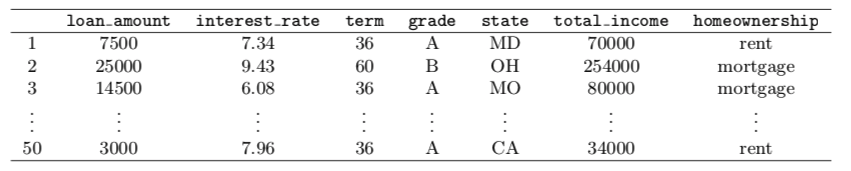
\includegraphics[scale=0.4]{datamatrix.png}
    \end{center}
    This \textbf{data matrix} shows rows 1, 2, 3, and 50 of a data set on loans. 
    \begin{itemize}
        \item Each row represents one loan.
        \item We call each row a \textbf{case} or \textbf{observational unit}. We \textit{observe} a number of different characteristics on each \textit{unit}.
        \item Each column represents some measured characteristic.
        \item We call these characteristics \textbf{variables} because they can \textit{vary} between observations. 
    \end{itemize}
\end{frame}

\begin{frame}{Understanding Our Data}
    \begin{center}
        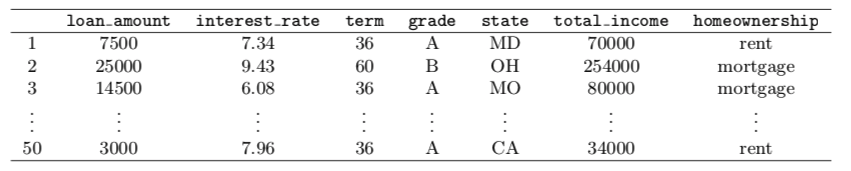
\includegraphics[scale=0.4]{datamatrix.png}
    \end{center}
    Whenever, we have data, it's important to start by making sure that we understand it. 
    \begin{itemize}
        \item What are some questions we might want to ask ourselves about this data set?
    \end{itemize}
\end{frame}

\begin{frame}{Understanding Our Data}
    Here are a few things I like to consider for all data sets:
    \begin{itemize}
        \item What does each variable represent?
        \item What are the units?
        \item Does the data make sense?
        \begin{itemize}
            \item What if the data showed an interest rate of $-999$?
            \item ...or a state labelled "42"?
        \end{itemize}
    \end{itemize}
\end{frame}

\begin{frame}{Types of Variables}
    Let's return to our data set:
    \begin{center}
        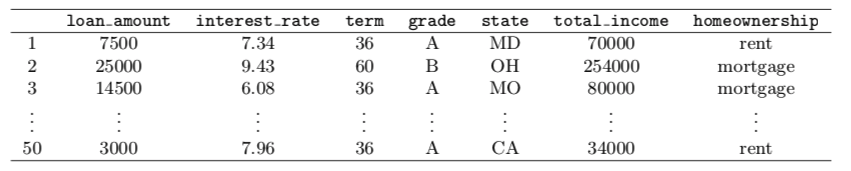
\includegraphics[scale=0.4]{datamatrix.png}
    \end{center}
    Notice that we have some variables made up of letters and some of numbers. This is the basic concept behind variable types. 
\end{frame}

\begin{frame}{Types of Variables}
    \begin{itemize}
        \item \textbf{Categorical}
        \begin{itemize}
            \item The responses are \textit{categories}.
            \item The state variable in our data set can take one of 50 possible values. 
        \end{itemize}
        \item \textbf{Numeric}
        \begin{itemize}
            \item The responses are \textit{numeric}.
            \item The numbers are meaningful (it makes sense to add, subtract, or take an average using those values). 
        \end{itemize}
    \end{itemize}
\end{frame}

\begin{frame}{Types of Numeric Variables}
    \begin{itemize}
        \item \textbf{Discrete}
        \begin{itemize}
            \item The responses can take on only whole number values.
            \item Population count is a discrete variable.
        \end{itemize}
        \item \textbf{Continuous}
        \begin{itemize}
            \item The responses can take on values on a continuous scale - there is no jump from one value to the next.
            \item Unemployment rate is a continuous variable. 
        \end{itemize}
    \end{itemize}
\end{frame}

\begin{frame}{Types of Variables}
    \begin{center}
        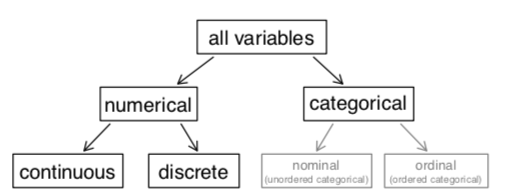
\includegraphics[scale=0.5]{vartypes.png}
    \end{center}
    Note: there are also two types of categorical variables.
    \begin{itemize}
        \item Ordinal variables are ordered (e.g., "like", "neutral", "dislike").
        \item Nominal variables are unordered (e.g., US states).
    \end{itemize}
\end{frame}

\begin{frame}{Relationships Between Variables}
    Our brains are constantly working on relationships between variables!
    \begin{itemize}
        \item Imagine if you walked down a flight of stairs outside your apartment 10 times and 9 of those times you fell down the stairs.
        \item You'd probably decide that something needs to change! Maybe you need to add some traction... or you need an extra cup of coffee before heading out in the morning. 
        \item In statistical terms, you decided that walking down those particular stairs relates to your falling down. You then make adjustments based on that association. 
    \end{itemize}
\end{frame}

\begin{frame}{Relationships Between Variables}
    Statistics takes these kinds of questions about how variables relate to one another (if I go out today, how likely am I to fall down the stairs?) and formalizes them so that we can make sound scientific claims.
\end{frame}

\begin{frame}{Relationships Between Variables}
    We can start thinking about how variables relate to one another through data visualization. 
    
    \begin{center}
        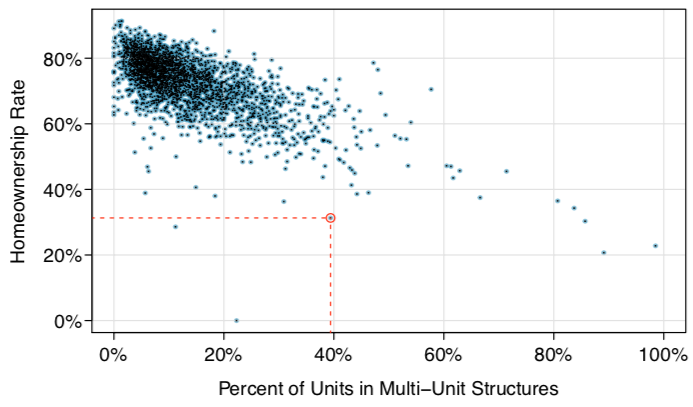
\includegraphics[scale=0.3]{scatter.png}
    \end{center}
    
    \vspace{-0.4cm}
    Consider the \textbf{scatterplot}. Do you think there's a relationship between a county's home ownership rate and its percent of units in multi-unit structures? Why might that be?
\end{frame}

\begin{frame}{Relationships Between Variables}
    \begin{center}
        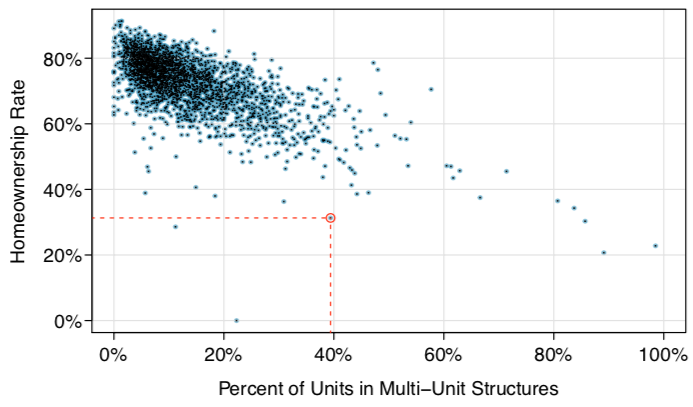
\includegraphics[scale=0.25]{scatter.png}
    \end{center}
    
    There is a clear pattern in the plot, so we say that these two variables are \textbf{associated}.
    \begin{itemize}
        \item Associated variables \textit{depend} on each other, so we say that they are \textbf{dependent variables}. 
        \item If two variables are not associated (no pattern), we say that they are \textbf{independent variables}.
    \end{itemize}
\end{frame}

\begin{frame}{Trend}
    \begin{center}
        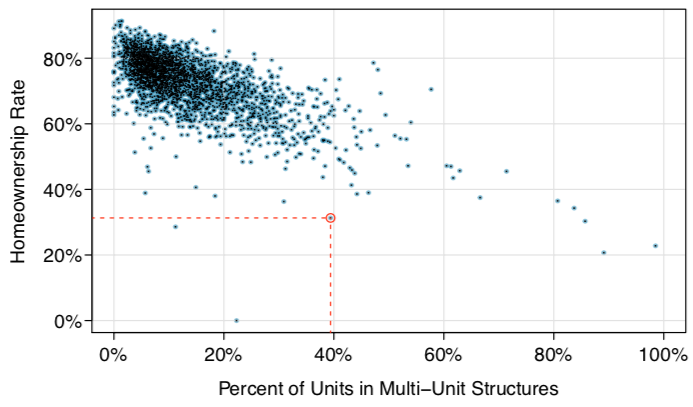
\includegraphics[scale=0.25]{scatter.png}
    \end{center}
    
    When two variables are related, we can consider the \textbf{trend}. 
    \begin{itemize}
        \item Here, there is a downward trend, suggesting that these two variables are \textbf{negatively associated}. 
        \item When we see an upward trend, we say that the variables are \textbf{positively associated}.
    \end{itemize}
\end{frame}

\begin{frame}{A Note on Correlation vs Causation}
    Who has heard someone say that "correlation is not causation"? 
    
    \vspace{1cm}
    Can you think of an example of two things that correlate but neither one causes the other?
\end{frame}

\begin{frame}{Correlation vs Causation}
    \begin{center}
        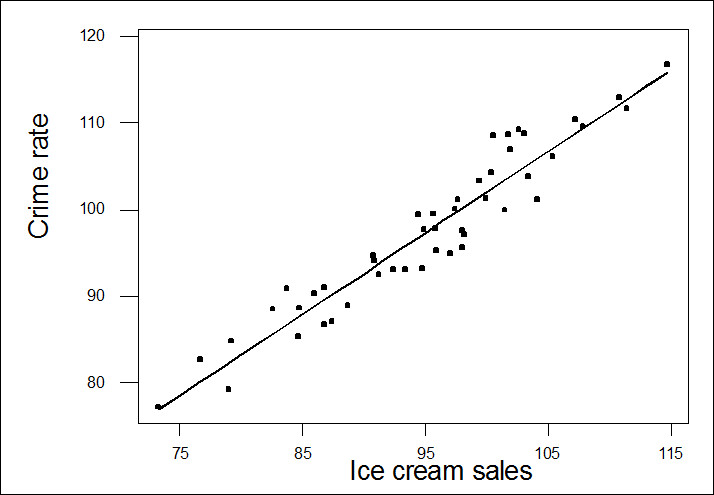
\includegraphics[scale=0.9]{icecream.jpeg}
    \end{center}
\end{frame}

\begin{frame}{Explanatory and Response Variables}
    Sometimes we do have causal questions. For example, suppose we have the following question:
    
    \begin{center}
        \textit{If there is an increase in the median household income in a county, does this drive an increase in its population?}
    \end{center}
    
    \begin{itemize}
        \item Median household income is an \textbf{explanatory variable}.
        \begin{itemize}
            \item We want to know if increases in median household income \textit{explain} population increases.
        \end{itemize}
        \item Population increase is a \textbf{response variable}.
        \begin{itemize}
            \item We want to know if the population increases \textit{in response to} increased median household income. 
        \end{itemize}
    \end{itemize} 
\end{frame}

\begin{frame}{Explanatory and Response Variables}
    When we predict some causal relationship, we can label our variables accordingly.
    
    \begin{center}
        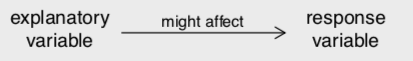
\includegraphics[scale=0.5]{affect.png}
    \end{center} 
    
    However, predicting causality and labeling variables as explanatory and response does \textit{not} guarantee that a causal relationship actually exists. 
    
    \vspace{12pt}
    (Remember our ice cream example - we can be wrong in our predictions but still find an association! )

\end{frame}
%\section{Section 1.3}
%\begin{frame}{Conducting Research}
    Statistics permeates research from start to finish! 
    \begin{itemize}
        \item The first step in any experiment is to design it.
        \item We design an experiment by deciding
        \begin{enumerate}
            \item What we want to know.
            \item Our target population (who or what we want to know about).
            \item The statistical methods we will use to analyze our data (this helps us decide what kind of data to collect).
        \end{enumerate}
    \end{itemize}
\end{frame}

\begin{frame}{Choosing How to Collect Data}
    A clear, specific research question can go a long way in helping to identify what subjects/cases are important and which variables we should measure. 
    
    \vspace{12pt}
    But we also need to consider \textit{how} these variables are measured.
\end{frame}

\begin{frame}{Research Questions}
    \begin{itemize}
        \item Research questions ask a question about some target \textbf{population}, which can be made up of anything we are interested in - people, dogs, bicycles, you name it.
        \item Typically we don't have access to every single person/dog/case in a population, so instead we look at a subset of the population. 
        \item This subset is called a \textbf{sample}. It is often a small fraction of the total population.  
    \end{itemize}
\end{frame}

\begin{frame}{Research Questions}
    Let's think about some possible research questions:
    \begin{enumerate}
        \item What is the average mercury content in swordfish in the Atlantic Ocean?
        \item Over the last 5 years, what is the average time to complete a degree for UCR undergrads?
        \item Does a new drug reduce the number of deaths in patients with severe heart disease?
    \end{enumerate}
    
    \vspace{12pt}
    What makes these research questions clear and specific? 
\end{frame}

\begin{frame}{Populations and Samples}
    What is the average mercury content in swordfish in the Atlantic Ocean?
    
    \begin{itemize}
        \item What is the target population in this research questions?
        \item What would represent an individual case?
    \end{itemize}
\end{frame}

\begin{frame}{Populations and Samples}
    What is the average mercury content in swordfish in the Atlantic Ocean?
    
    \begin{itemize}
        \item What is the target population in this research questions?
        \begin{itemize}
            \item All swordfish in the Atlantic Ocean.
        \end{itemize}
        \item What would represent an individual case?
        \begin{itemize}
            \item Each individual swordfish in the Atlantic Ocean.
        \end{itemize}
    \end{itemize}
\end{frame}

\begin{frame}{Populations and Samples}
    Discuss with a neighbor and jot down your thoughts on our other two research question examples. What is the target population in each research question? What represents an individual case?
    
    \vspace{12pt}
    1. Over the last 5 years, what is the average time to complete a degree for UCR undergrads?
    
    2. Does a new drug reduce the number of deaths in patients with severe heart disease?
    
\end{frame}

\begin{frame}{Populations and Samples}
    1. Over the last 5 years, what is the average time to complete a degree for UCR undergrads?
    \begin{itemize}
        \item Population: all UCR undergrads
        \item Individual case: each UCR undergrad
    \end{itemize}
\end{frame}

\begin{frame}{Populations and Samples}
    2. Does a new drug reduce the number of deaths in patients with severe heart disease?
    \begin{itemize}
        \item Population: all patients with severe heart disease
        \item Individual case: each patient with severe heart disease
    \end{itemize}
\end{frame}

\begin{frame}{Anecdotal Evidence}
    Consider the following:
    \begin{enumerate}
        \item I ate Atlantic swordfish and got mercury poisoning, so the mercury levels must really high. 
        \item I know of two UCR undergrads who took 8 years to graduate, so it must take an unusually long time to graduate from UCR.
        \item My dog took a new heart disease drug and hasn't had a heart attack, so it must work.
    \end{enumerate}
\end{frame}

\begin{frame}{Anecdotal Evidence}   
    \vspace{12pt}
    Each claim on the previous slide is based on data! But...
    \begin{enumerate}
        \item The sample sizes are very small!
        \item Even if we manage to verify these claims (e.g., the mercury poisoning was actually caused by swordfish), we have no way of knowing if they represent the population well or are extreme cases.
        \item We often remember only the extreme cases because they are striking (or possibly due to expectation bias).
    \end{enumerate}
    
    \vspace{12pt}
    Can you think of a time when you heard someone to use \textbf{anecdotal evidence} to demonstrate a point?
\end{frame}

\begin{frame}{Sampling from a Population}
    One we've established our target population and what constitutes an individual case, it's time to think about collecting a sample. 
    
    \vspace{12pt}
    For our question about UCR time-to-graduation, recall that
    \begin{itemize}
        \item our \textit{population} is all UCR undergrads
        \item and our \textit{sample} is made up of whatever graduated students we selected for review.
    \end{itemize}
\end{frame}
 
\begin{frame}{Sampling from a Population}    
    \vspace{12pt}
    What if we took a sample of everyone in an upper division physics course? Are these students likely to be representative of UCR students \textit{on average}?
\end{frame}
 
\begin{frame}{Sampling from a Population}     
    \vspace{12pt}
    If we select samples this way, we are likely to get a \textbf{biased} sample. In this case, we would \textit{bias} the sample toward however long it takes physics students to graduate. 
\end{frame}

\begin{frame}{Sampling from a Population}
    In order to get a sample that represents UCR students overall, we want to \textit{randomly} sample from our population of all graduated UCR undergrads.
    
    \vspace{12pt}
    Think of a random sample as a raffle. Each graduated UCR student from the past 5 years get a raffle ticket, and 100 of them are selected randomly. We then ask these 100 students how long they took to graduate. 
\end{frame}

\begin{frame}{The Simple Random Sample}
    The most straightforward way to collect a random sample is the \textbf{simple random sample}. This is essentially equivalent to the raffle example:
    \begin{itemize}
        \item Each case in the population has an equal probability of being included in the sample.
        \item There is no connection between cases in the sample.
    \end{itemize}  
\end{frame}

\begin{frame}{Sources of Bias}
    \textbf{Bias} can occur in simple random samples due to individuals not responding. 
    
    \vspace{12pt}
    If students who took 6 or more years to graduate also happen to be less likely to respond, we may end up with data to suggest that our average time-to-graduation is quicker than it actually is. 
\end{frame}

\begin{frame}{Sources of Bias}   
    \vspace{12pt}
    Usually bias occurs in a sample when we do something out of convenience instead of going through all of the steps to get a truly random sample. 
    
    \vspace{12pt}
    A \textbf{convenience sample} is where individuals are sampled because it's easy. E.g., you sample everyone in this class instead of trying to randomly sample from all UCR students. 
\end{frame}

\begin{frame}{Bias in the Wild: Amazon Reviews}
    \begin{columns}[T] % align columns
    \begin{column}{.48\textwidth}
        \vspace{2cm}
        
        Suppose you're looking for a new outfit for your pet lizard. You find what appears to be the perfect outfit on Amazon, but the reviews are pretty mixed.
    \end{column}%
    \hfill%
    \begin{column}{.48\textwidth}
    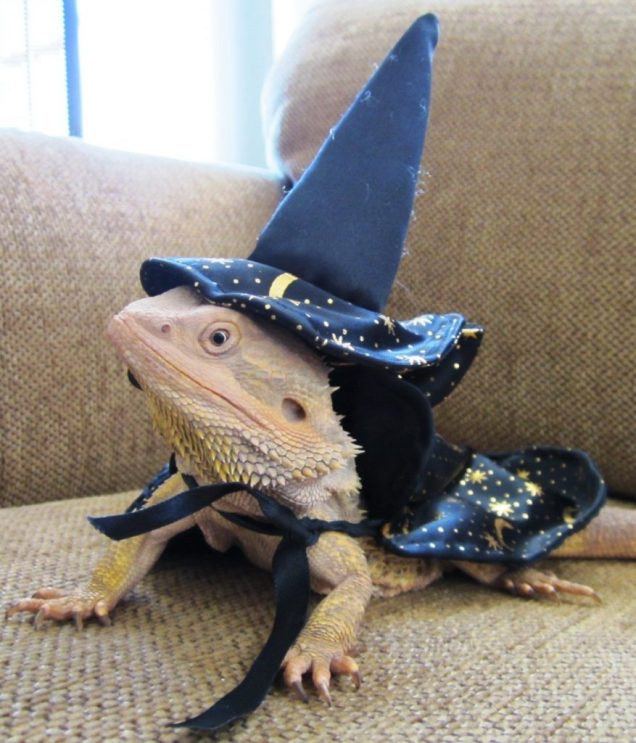
\includegraphics[scale=0.25]{images/lizard.jpg}
    \end{column}%
    \end{columns}
\end{frame}

\begin{frame}{Bias in the Wild: Amazon Reviews}
        \begin{columns}[T] % align columns
    \begin{column}{.48\textwidth}
        \vspace{2cm}
    
        Do you think the reviews give an accurate representation of how buyers feel about this item? When do you think people are more likely to leave reviews?
    \end{column}%
    \hfill%
    \begin{column}{.48\textwidth}
    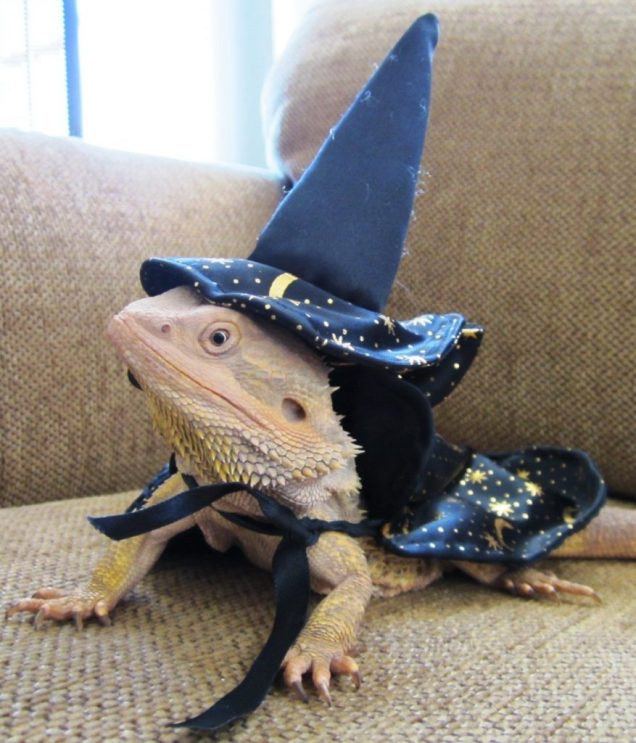
\includegraphics[scale=0.25]{images/lizard.jpg}
    \end{column}%
    \end{columns}
\end{frame}

\begin{frame}{Observational Studies}
    Data where no treatment is explicitly applied (or withheld) is \textbf{observational data}. 
    \begin{itemize}
        \item These kinds of studies are \textit{non-experimental}.
        \item It is difficult to make causal claims based on observational data.
        \item Instead, we can use observational studies to 
        \begin{itemize}
            \item form hypotheses for future experiments.
            \item demonstrate associations (that may or may not be causal).
        \end{itemize}
    \end{itemize}
\end{frame}

\begin{frame}{Examples of Observational Studies}
    \begin{itemize}
        \item Relationship between smoking and lung health.
        \begin{itemize}
            \item Here, smoking is the "treatment".
            \item Ethical constraints prevent us from randomly assigning people to smoking or nonsmoking.
        \end{itemize}
        \item Relationship between gender and number of pets.
        \begin{itemize}
            \item Here, gender is the "treatment".
            \item We can't impose a gender on someone, so we are unable to randomly assign gender.
        \end{itemize}
    \end{itemize}
\end{frame}

\begin{frame}{Observational Studies}
    Can you think of something you might be interested in studying where "treatment" can't be explicitly applied? 
    
    \vspace{18pt}
    How do you think we deal with some of the ethical constraints like those in the smoking study? 
\end{frame}

\begin{frame}{Why No Causal Claims?}
    Consider an observational study that tracked sunscreen use versus skin cancer. The study found that the more sunscreen someone used, the more likely they were to develop skin cancer. 
    
    \begin{itemize}
        \item Does sunscreen use cause skin cancer?
        \item What information could we be missing?
    \end{itemize}
\end{frame}

\begin{frame}{Sunscreen and Skin Cancer}
    \begin{itemize}
        \item This missing information consists of variables that we didn't measure.
        \textbf{Confounding variables} are variables that are correlated with (have a relationship with) both the explanatory and response variables.
        \item Confounding variables can help explain why unexpected relationships occur.
        \item It is almost impossible to guarantee that we've measured (or even thought of) all confounding variables.
        \item Note: just because a relationship makes sense, doesn't mean it is causal or that there are no confounding variables!
    \end{itemize}
\end{frame}

\begin{frame}{Types of Observational Studies}
    We can ask two types of observational questions. 
    \begin{itemize}
        \item A \textbf{prospective study} collects data as the events unfold.
        \item A \textbf{retrospective study} collects data on events that have already taken place. 
    \end{itemize}
    
    Some datasets may include variables taken both prospectively and retrospectively. 
\end{frame}

\begin{frame}{Sampling Methods}
    \textbf{Simple random sampling} is the "raffle method" we talked about earlier. Each case has an equal probability of being selected from the population.
    
    \vspace{18pt}
    \textbf{Stratified sampling} uses a "divide-and-conquer" approach. 
    \begin{itemize}
        \item The population is divided into groups called \textbf{strata}, chosen so that similar cases are grouped together.
        \begin{itemize}
            \item We could group based on variables like year in college, gender, team, etc.
            \item We typically choose these grouping based on some variable that we think relates to our outcome. 
        \end{itemize}
        \item We then randomly sample a fixed number of cases from each strata. 
    \end{itemize}
\end{frame}

\begin{frame}{Sampling Methods}
    \textbf{Cluster sampling} involves breaking the population into many groups, called \textbf{clusters}. 
    \begin{itemize}
        \item We then randomly select some of the clusters and sample all of the cases in each of the selected clusters.
    \end{itemize}
    
    \vspace{18pt}
    \textbf{Multistage sampling} is similar to cluster sampling, but instead of keeping all cases in each cluster, we randomly sample from each selected cluster (this is the "multistage" part). 
\end{frame} 

\begin{frame}{Sampling Methods}
    Cluster and multistage sampling may be cheaper and easier to collect.
    \begin{itemize}
        \item If we wanted to sample individuals from 30 remote villages, it would be cheaper to cluster by village and only travel to 10 of them. 
    \end{itemize}
    We may also use these approaches when within-cluster variability is high but the clusters are similar \textit{on average}. 
    \begin{itemize}
        \item For example, 5 economically diverse neighborhoods with similar average wages in each neighborhood. 
    \end{itemize}
    
    \vspace{18pt}
    The analyses discussed in this class will all pertain to simple random sampling. However, most of these analyses can be extended to work with a variety of sampling methods. 
\end{frame}
%\section{Section 1.4}
%\begin{frame}{Experiments}
    Studies where researchers assign treatments to cases are \textbf{experiments}. 
    
    \vspace{12pt}
    Whenever an experiment utilizes randomly assigned treatments, we say that it is a \textbf{randomized experiment}. 
    
    \begin{itemize}
        \item Note: "treatment" refers to whatever explanatory variable we are most interested in. 
    \end{itemize}
\end{frame}

\begin{frame}{Principles of Experimental Design}
    Four key principles:
    \begin{enumerate}
        \item Controlling
        \item Randomization
        \item Replication
        \item Blocking
    \end{enumerate}
\end{frame}

\begin{frame}{Principles of Experimental Design: Controlling}
    When treatments are assigned to cases, researchers do their best to \textbf{control} any other differences in the treatment groups. 
    \begin{itemize}
        \item For example, if both groups are given a pill to take with water, we might instruct everyone to drink the full 8 oz of water in order to control for any impact of water consumption.
    \end{itemize}
\end{frame}

\begin{frame}{Principles of Experimental Design: Randomization}
    Researchers \textbf{randomize} cases into treatment groups.
    \begin{itemize}
        \item This helps account for any unmeasured variables.
        \item For example, if we're studying a new cancer therapy and dog ownership has a positive impact on cancer outlook, randomization helps ensure that we have similar numbers of dog owners in each treatment group. 
        \item This helps minimize bias in our data. 
    \end{itemize}
\end{frame}

\begin{frame}{Principles of Experimental Design: Replication}
    The more information we have, the more confident we can be in our results! We gather more information through \textbf{replication}. 
    \begin{itemize}
        \item Suppose we have 3 treatment groups. Replication is just testing each treatment multiple times (multiple cases are assigned to each treatment group). 
    \end{itemize}
\end{frame}

\begin{frame}{Principles of Experimental Design: Blocking}
    If we suspect (or know) that other variables are important in influencing a response, we can group cases into \textbf{blocks}.
    \begin{itemize}
        \item Cases within each block are then randomly assigned to each treatment. 
        \item For example, if we are looking at a new asthma medication, we might block individuals by high, medium, and low severity of asthma. Then half of the individuals in each block would be assigned to the new medication. 
        \item This helps ensure that each treatment group has similar numbers of patients from each severity level. 
    \end{itemize}
\end{frame}

\begin{frame}{Principles of Experimental Design}
    \begin{itemize}
        \item All experiments will use some form of controlling, randomization, and replication. 
        \item Blocking is a slightly more advanced technique (in that it requires slightly more advanced methods to analyze). 
        \item You will learn more about blocking if you take STAT 100B. 
    \end{itemize}
\end{frame}

\begin{frame}{Bias in Human Experiments}
    Randomized experiments are the gold standard, but even they have their limitations!
    
    \vspace{12pt}
    Experiments involving people are especially prone to bias.
\end{frame}

\begin{frame}{Example: Heart Attack Drugs}
    Suppose we are interested in whether a new drug helps to prevent repeated cardiac events in patients who have already had at least one heart attack. 
    
    \begin{itemize}
        \item We get a random sample of 100 people who have had a heart attack in the past. 
        \item 50 of them are randomly assigned to the treatment (our new drug). This is our \textbf{treatment group}.
        \item The other 50 do not receive the drug. This is our \textbf{control group}. 
    \end{itemize}
    
    Can you think of anything that could bias our results?
\end{frame}

\begin{frame}{Sources of Bias}
    \begin{itemize}
        \item People who get the new drug expect it to work.
        \item E.g., people who did not get the drug may wonder if their study participation was worth the risk.
        \item Doctors may inadvertently affect the results through their optimism (or lack thereof) when administering the drug. 
    \end{itemize}
\end{frame}

\begin{frame}{Reducing Bias in Human Experiments}
    We can reduce bias by 
    \begin{itemize}
        \item Keeping patients uninformed about their treatment group.
        \begin{itemize}
            \item We call these studies \textbf{blind}.
            \item One way to keep studies blind is to give the control group a \textbf{placebo}.
        \end{itemize}
        \item Keeping doctors uninformed about which treatment groups their patients are in.
        \begin{itemize}
            \item We call these studies, where neither patient nor medical provider know the treatment group, \textbf{double-blind}. 
        \end{itemize}
    \end{itemize}
    
    \vspace{12pt}
    Can you think of some ethical issues that may arise in randomized, double-blind, placebo-controlled studies?
\end{frame}

%\section{Section 2.1}
%\begin{frame}{Summarizing Data}
    Chapter 2 is all about summarizing data through summary statistics and graphs. We can get a lot of information out of these things!
    
    \vspace{12pt}
    These concepts are also important foundations for the rest of the course.
\end{frame}

\begin{frame}{Numerical Data}
    Let's start by thinking of a simple numeric variable: the ages of everyone in this room.
    
    \vspace{18pt}
    Can you think of any ways to summarize all of our ages in only one or two numbers?
\end{frame}

\begin{frame}{Scatterplots}
    A \textbf{scatterplot} shows a case-by-case view of two numerical variables. 
    
    \begin{center}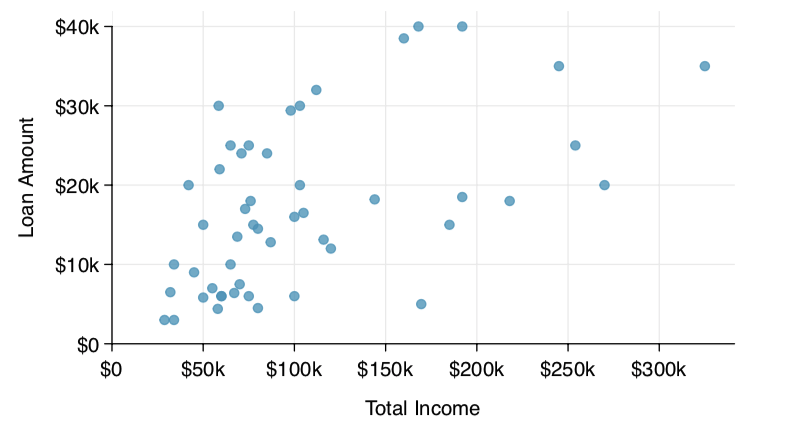
\includegraphics[scale=0.3]{images/scatter2.png}\end{center}
    
    What can we learn from the scatterplot?
\end{frame}

\begin{frame}{Dot Plots}
    A \textbf{dot plot} is like a scatterplot with only one variable. It shows how a single, \textit{continuous} numerical variable falls on a number line. 
    
    \begin{center}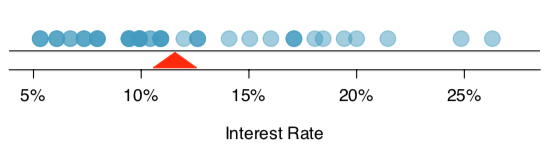
\includegraphics[scale=0.5]{images/dotplot.png}\end{center}
    
\end{frame}

\begin{frame}{Dot Plots}
    A \textbf{stacked dot plot} shows the same information for a \textit{discrete} numerical variable.   
    
    \begin{center}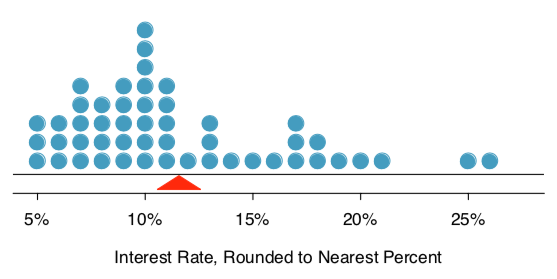
\includegraphics[scale=0.5]{images/dotplot2.png}\end{center}
\end{frame}

\begin{frame}{Histograms}
    A \textbf{histogram} is similar to a dot plot, but instead of showing the exact value for each observation, values are put into \textbf{bins}.
    
    \begin{center}
        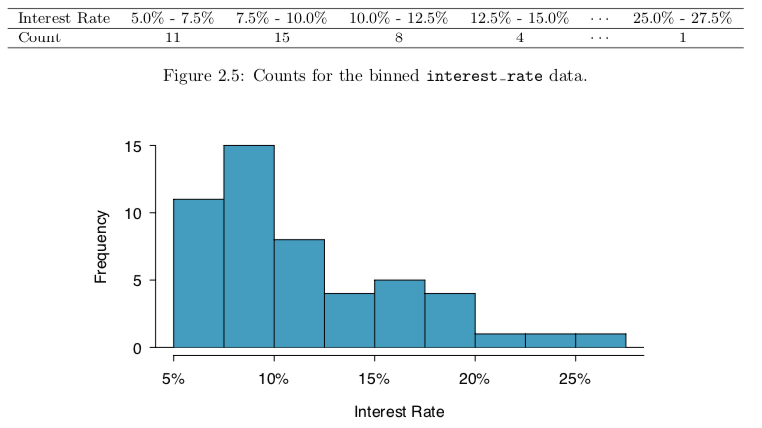
\includegraphics[scale=0.4]{images/hist1.png}
    \end{center}
\end{frame}

\begin{frame}{The Mean}
    Both of the dot plots had a red arrow pointing to the \textbf{mean} (or \textbf{average}) of the variable. 
    
    \vspace{12pt}
    You've probably calculated an average before, but if you haven't (or if you need a refresher), to find the mean you add all of the values and then divide by the number of values. 
\end{frame}

\begin{frame}{The Mean}
    For example, if we had a variable called \texttt{ages} with the values 21, 22, 26, 18, 19, and 21, the mean would be
    \vspace{12pt}
    \[
    \frac{\text{sum of values}}{\text{total \# of observations}} = \frac{21+22+26+18+19+21}{6}.
    \]
    
    \vspace{12pt}
    We denote the mean by $\boldsymbol{\bar{x}}$. In this case, $\bar{x}=21.167$
\end{frame}

\begin{frame}{The Mean}
    In math notation, the formula for the mean looks like this:
    \[
        \bar{x} = \frac{1}{n}\sum_{i=1}^n x_i = \frac{x_1 + x_2 + \dots + x_n}{n}.
    \]
    
    \vspace{12pt}
    In our example, $n=6$ observations and each $x_i$ is one of our ages.
\end{frame}

\begin{frame}{Measures of Center}
    The mean is a common way to measure the center (middle) of the \textbf{distribution} of the data.
    
    \vspace{12 pt}
    You can think of the distribution as the way that the data is \textit{distributed} from left to right on a histogram.
\end{frame}

\begin{frame}{Measures of Center}
    The mean of a variable is denoted by $\bar{x}$. This is what we refer to as the \textbf{sample mean}. 
    
    \vspace{12pt}
    The mean of the entire population is typically something that we don't have exact data on (we usually don't have data for every single member of a population). Instead, we estimate the population mean using a sample mean.
    
    \vspace{12pt}
    The \textbf{population mean} is denoted by $\boldsymbol{\mu}$. This is the Greek letter \textit{mu}.
\end{frame}

\begin{frame}{That's a lot of symbols to remember?}
    Let's put them all in one place. We will add to this list as we go.
    \begin{itemize}
        \item $n$: number of observations/cases
        \item $\bar{x}$: sample mean
        \item $\mu$: population mean
    \end{itemize}
\end{frame}

\begin{frame}{Data Density}
    Now that we've brought up the distribution of the data, we can start to think about the density of the data.
    
    \vspace{12pt}\textbf{Data density} refers to the amount of data in any bin. (Taller bins mean more data density, or more data in the bin.)
    
    \vspace{12pt}From here, we can start to consider the \textit{shape} of a distribution. 
\end{frame}

\begin{frame}{Shape}
    Remember our histogram?
    
    \begin{center}
        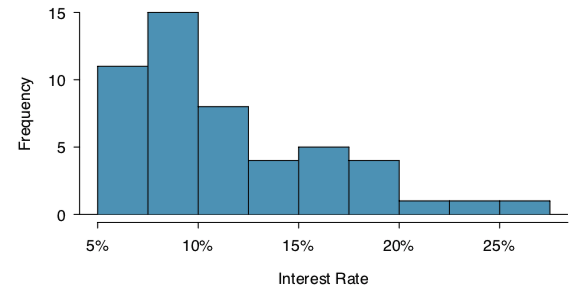
\includegraphics[scale=0.3]{images/hist2.png}
    \end{center}
    
    \begin{itemize}
        \item The sides of the distribution (on either side of the mean) are referred to as the \textbf{tails}. 
        \item Here the data have a long, thin right tail, so we say that the shape is \textbf{right skewed}. 
    \end{itemize}
\end{frame}

\begin{frame}{Shape}
    \begin{itemize}
        \item If the data have a long, thin tail on the left, we say that the shape is \textbf{left skewed}.
        \item If the data have roughly equal tails, we say the distribution is \textbf{symmetric}. 
    \end{itemize}
\end{frame}

\begin{frame}{Shape}
    We can also talk about the modes of a distribution. In a distribution, a \textbf{mode} is any prominent peak in the distribution. These can be found in a histogram! 
    \begin{itemize}
        \item A distribution with one prominent peak is called \textbf{unimodal}.
        \item Distributions with two prominent peaks are \textbf{bimodal}.
        \item Distributions with three or more promiment peaks are \textbf{multimodal}. 
    \end{itemize}
\end{frame}

\begin{frame}{Modes}
    \begin{center}
        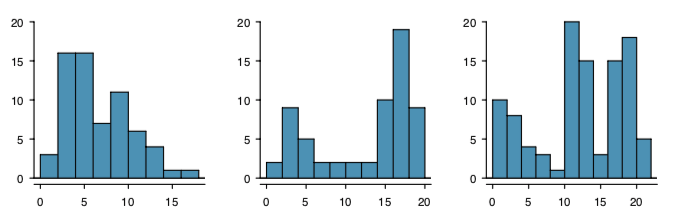
\includegraphics[scale=0.5]{images/modes.png}
    \end{center}
    
    How many modes are there in each distribution? \\ Remember that we only count \textit{prominent} peaks.
\end{frame}

\begin{frame}{Modes}
    Bin widths, our particular sample, and differing opinions can all impact where we see a "prominent" mode.
    
    \vspace{12pt} ...but that is okay! The goal of examining the shape of our data is simply to better understand the nature of our data. This allows us to make more informed technical decisions down the line. 
\end{frame}

\begin{frame}{Variability}
    We talked about the mean as a way to measure the center of the data, but the variability of data is also an important consideration. 
    
    \vspace{12pt}
    Why might the variability be important?
\end{frame}

\begin{frame}{Why Variability?}
    Suppose we want to know the average age in this class and take two random samples of size 10 each. 
    
    \begin{table}[]
    \begin{tabular}{ll}
    Sample 1: & 22, 19, 20, 18, 20, 21, 20, 22, 20, 18\\ 
    \hline
    Sample 2: & 12, 18, 32, 21, 19, 19, 17, 21, 22, 19
    \end{tabular}
    \end{table}

    In both cases, we get a sample average of $\bar{x}=20$.
    
    \vspace{12pt}How confident are you about our estimate of the average age in this class using Sample 1? What about Sample 2?
\end{frame}

\begin{frame}{Variability}
    We can think about variability as how far away the observations are from the mean. 
    
    \vspace{12pt}The distance between an observation and its mean is called the \textbf{deviation}. From Sample 1 (22, 19, 20, 18, 20, 21, 20, 22, 20, 18), the deviations for the first, second, and tenth observations are
    \begin{align*}
        x_1 - \bar{x} &= 22-20 = 2 \\
        x_2 - \bar{x} &= 19-20 = -1 \\
        x_{10}-\bar{x} &= 18-20=-2
    \end{align*}
\end{frame}

\begin{frame}{Variability}
    We're interested in how far a typical observation is from the mean, but if we add up all of the deviations for a sample, we always get zero! Let's try it on Sample 1:
    
    \begin{align*}
        & (x_1 - \bar{x}) + (x_2 - \bar{x}) + \dots + (x_9 - \bar{x}) + (x_{10} - \bar{x}) \\
        &= (22-20) + (19-20) + (20-20) + (18-20) + (20-20) \\ & \quad + (21-20) + (20-20) + (22-20) + (20-20) + (18-20) \\
        &= 2 + (-1) + 0 + (-2) + 0 + 1 + 0 + 2 + 0 + (-2) \\
        &= 2 - 1 - 2 + 1 + 2 - 2 \\
        &= 0
    \end{align*}
    
    Note: A short proof of this will be posted on the course website.
\end{frame}

\begin{frame}{Variability}
    So the average deviance doesn't work... 
    \begin{itemize}
        \item This is because all of those positives and negatives end up balancing each other out. 
        \item When we talk about variability, we aren't that interested in whether any particular point is above or below the mean.
        \item We really just want to know how far away it is.
    \end{itemize}
\end{frame}

\begin{frame}{Variability}
    There are two simple ways to get rid of the signs to focus on distance (without direction).
    \begin{enumerate}
        \item Take the absolute value of the number.
        \item Square the number.
    \end{enumerate}
    
    \vspace{12pt}It turns out that there are a whole lot of mathematical reasons why it's easier to work with squares than with absolute values!
\end{frame}

\begin{frame}{Variance}
    And so we come to the \textbf{variance}. The variance can be inconvenient to calculate by hand, but it goes something like this:
    \begin{enumerate}
        \item We square all of those deviations we calculated previously.
        \item Add them up.
        \item Take the average.
    \end{enumerate}
    We denote our \textbf{sample variance} by $\boldsymbol{s^2}$.
\end{frame}

\begin{frame}{Variance}    
    \vspace{12pt}Note: Technically, we divide by $n-1$ instead of by $n$ when we take our average. We may talk more about this later, but in the meantime just know that there's some mathematical nuance that makes the variance formula a little bit more complicated. 
\end{frame}

\begin{frame}{Variance}
    Let's return to our example and Sample 1. We already calculated our deviations, but this time we square them before adding them up.
    \begin{align*}
        & (22-20)^2 + (19-20)^2 + \dots + (20-20)^2 + (18-20)^2 \\
        & = 2^2 + (-1)^2 + 0^2 + (-2)^2 + 0^2 + 1^2 + 0^2 + 2^2 + 0^2 + (-2)^2 \\
        &= 4 + 1 + 4 + 1 + 4 + 4 \\
        &= 18
    \end{align*}
    And then we divide by $n-1=9$
    \[
    \frac{18}{9}=2.
    \]
\end{frame}

\begin{frame}{Standard Deviation}
    The variance can be described as the average squared distance from the mean. That probably doesn't sound like a very intuitive way to measure variability.
    
    \vspace{12pt}However, the \textbf{standard deviation} is easier to conceptualize than the variance: it gets at our original goal of estimating how far a typical observation is from the mean.
\end{frame}

\begin{frame}{Standard Deviation}
    Fortunately for us, the standard deviation doesn't require any additional mathematical nuance! In order to calculate the standard deviation, we simply take the square root of the variance.
    
    \vspace{12pt}Returning again to our example, 
    \[
    s = \sqrt{s^2} = \sqrt{2} \approx 1.414
    \]
\end{frame}

\begin{frame}{Standard Deviation}
    In general,
    \begin{itemize}
        \item 70\% of the data will fall within one standard deviation of the mean.
        \item 95\% of the data will fall within two standard deviations of the mean.
    \end{itemize}
    ...but these are not strict rules!
\end{frame}

\begin{frame}{Population Variability}
    Like the mean, the \textbf{sample variance} and \textbf{sample standard deviation} also have population counterparts.
    \begin{itemize}
        \item The \textbf{population variance} is denoted $\boldsymbol{\sigma^2}$.
        \item The \textbf{population standard deviation} is denoted $\boldsymbol{\sigma}$.
    \end{itemize}
    $\sigma$ is the Greek letter \textit{sigma}. (We often use Greek letters to denote values from our population.)
\end{frame}

\begin{frame}{Mean and Standard Deviation}
    Much of what we do in statistics is (1) estimate quantities and (2) determine how uncertain we are about those estimates. 
    \begin{itemize}
        \item The mean is often a quantity of interest.
        \item The standard deviation helps us determine how uncertain we are about this quantity.
    \end{itemize}
    
    \vspace{12pt}We will talk more about uncertainty in Chapter 5.
\end{frame}

\begin{frame}{Symbols to Remember}
    Let's update our list with variance and standard deviation.
    \begin{itemize}
        \item $n$: number of observations/cases
        \item $\bar{x}$: sample mean
        \item $\mu$: population mean
        \item $s^2$: sample variance
        \item $s$: sample standard deviation
        \item $\sigma^2$: population variance
        \item $\sigma$: population standard deviation
    \end{itemize}
\end{frame}

\begin{frame}{Mean, Standard Deviation, and Shape}
    Mean, standard deviation, and shape together give us a good description of our distribution. 
    \begin{itemize}
        \item If any one of these is missing, we miss crucial information.
        \item Without the mean, we lack information about the center of the distribution.
        \item Without the standard deviation, we are unable to capture how spread out the data are. 
    \end{itemize}
\end{frame}

\begin{frame}{Why Shape?}
    These three distributions have the same mean ($\bar{x}=0$) and standard deviation ($s=1$)!
    \begin{center}
        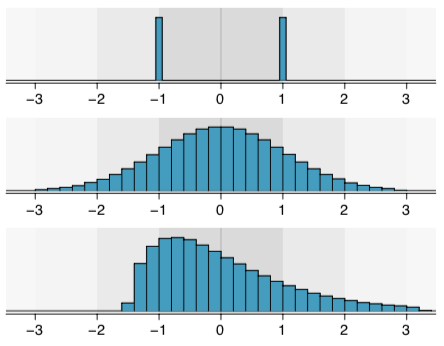
\includegraphics[scale=0.35]{images/shapes.png}
    \end{center}
    A good description of shape should include modality and skewness (or symmetry). To give an even clearer picture, we can report where the modes are and the sharpness of the peaks.
\end{frame}

\begin{frame}{Box Plots}
    \begin{center}
        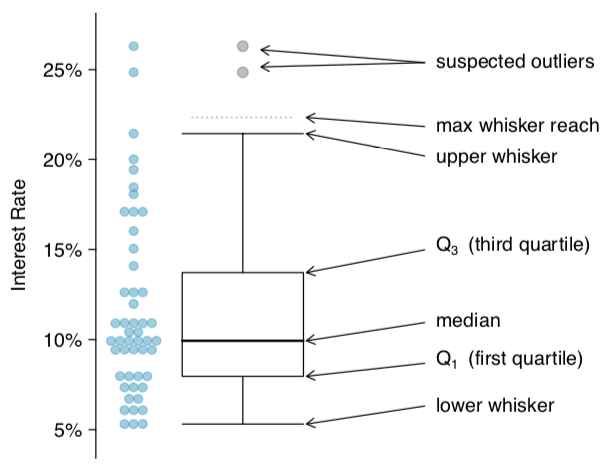
\includegraphics[scale=0.4]{images/boxplot.png}
    \end{center}
    A stacked dot plot next to a vertical box plot. 
\end{frame}

\begin{frame}{The Median}
    The first step in constructing a box plot is to draw a line at the median. 
    
    \begin{center}
        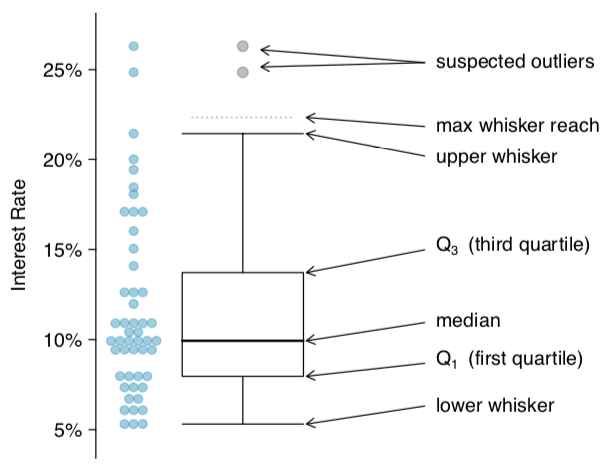
\includegraphics[scale=0.35]{images/boxplot.png}
    \end{center}
\end{frame}

\begin{frame}{The Median}
    \begin{itemize}
        \item The \textbf{median} takes the data and splits it in half. 
        \item The median is also called the \textbf{50th percentile} because 50\% of the data is below this value.
        \item The median is another measure of center. 
        \item To find the median, we sort our numerical variable and then find the halfway point.
    \end{itemize}
\end{frame}

\begin{frame}{The Median}
    If we have an odd number of observations, say,
    \[
        1,2,3,4,5
    \]
    we take the observation in the middle (the $\frac{n+1}{2}$th observation).
   
   \vspace{12pt}In this case,
    \[
        1,2,\boldsymbol{3}, 4, 5
    \]
    3 is the median. 
\end{frame}

\begin{frame}{The Median}
    \begin{itemize}
        \item If we have an even number of observations
        \[
        1,2,3,4,5,6
        \]
        we cut the data exactly in half
        \[
        1,2,3 \quad|\quad 4,5,6
        \]
        and the median is the average of the two observations closest to the halfway point
        \[
        \frac{3+4}{2}=3.5
        \]
    \end{itemize}
\end{frame}

\begin{frame}{Quartiles}
    The next step in our box plot is to draw a box connecting the first and third quartiles.
    
    \begin{center}
        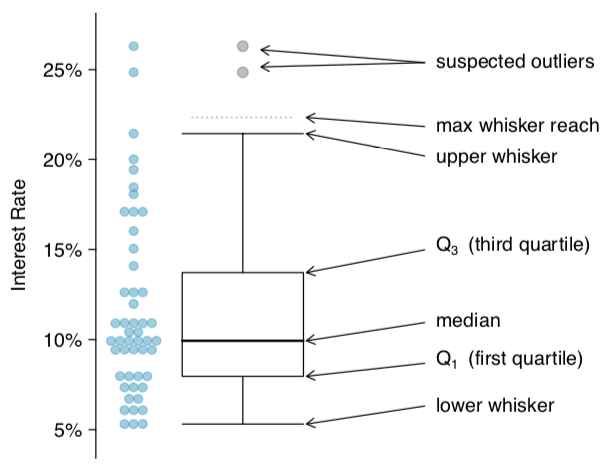
\includegraphics[scale=0.35]{images/boxplot.png}
    \end{center}
\end{frame}

\begin{frame}{Quartiles}
    \textbf{Quartiles} split our data into \textit{quarters}.
    \begin{itemize}
        \item 25\% of the data falls below the \textbf{first quartile} (Q1). 
        \begin{itemize}
            \item This is the 25th percentile. 
        \end{itemize}
        \item 50\% of the data falls below the median.
        \item 75\% of the data falls below the \textbf{third quartile} (Q3). 
        \begin{itemize}
            \item This is the 75th percentile. 
        \end{itemize}
    \end{itemize}
    
    \vspace{12pt}What percent of the data falls between Q1 and the median? What percent between Q1 and Q3?
\end{frame}

\begin{frame}{Finding Quartiles}
    \begin{enumerate}
        \item Find the median.
        \item Take all of the data that falls \textit{below} the median and find the middle of that data using the same steps we used to find the median. This is the first quartile.
        \item Repeat with the data that falls \textit{above} the median. This is the third quartile.
    \end{enumerate}
\end{frame}

\begin{frame}{Interquartile Range}
    \begin{itemize}
        \item The distance between the first and third quartiles is referred to as the \textbf{interquartile range} (or IQR).
        \item This value is easy to calculate!
        \[
        IQR = Q3 - Q1
        \]
        \item The IQR is another measure of variability.
    \end{itemize}
\end{frame}

\begin{frame}{Whiskers}
    Now we need to find the whiskers.
    \begin{center}
        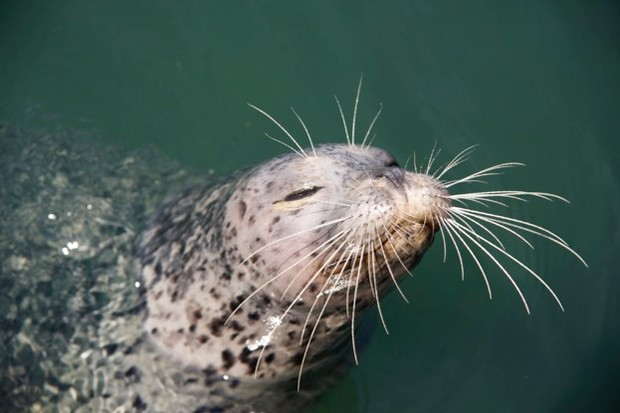
\includegraphics[scale=0.4]{images/whiskers.jpg}
    \end{center}
    \flushright\tiny{Image from BBC Wildlife \\ www.discoverwildlife.com/animal-facts/mammals/how-do-whiskers-work/}
\end{frame}

\begin{frame}{Whiskers}
    Now we need to find the whiskers.
    \begin{center}
        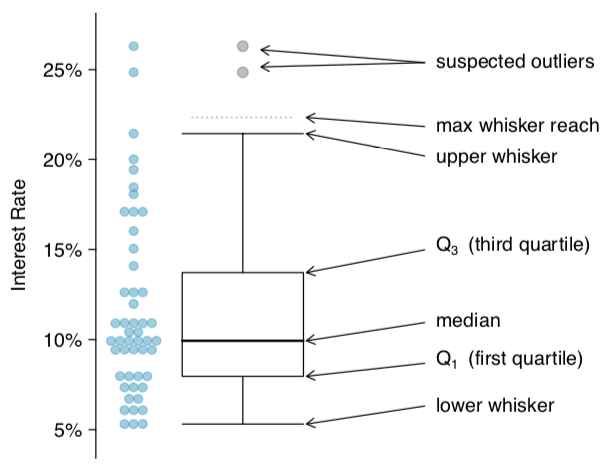
\includegraphics[scale=0.35]{images/boxplot.png}
    \end{center}
\end{frame}

\begin{frame}{Whiskers}
    The \textbf{whiskers} capture (most of) the rest of the data.
    \begin{itemize}
        \item Each whisker is no longer than 
        \[
        1.5\times IQR.
        \]
        and stops at the point closest to, but still within, this range.
    \end{itemize}
\end{frame}

\begin{frame}{Whiskers}
    \begin{itemize}
        \item The upper whisker goes no farther than
        \[
        Q3 + 1.5 \times IQR
        \]
        and the lower whisker no farther than
        \[
        Q1 - 1.5 \times IQR
        \]
    \end{itemize}
    
    We may choose not to include the maximum upper reach and minimum lower reach on our box plot, but we always include the whiskers themselves. 
\end{frame}

\begin{frame}{Outliers}
    Finally, we add any outliers by labeling each one with a dot.
    \begin{center}
        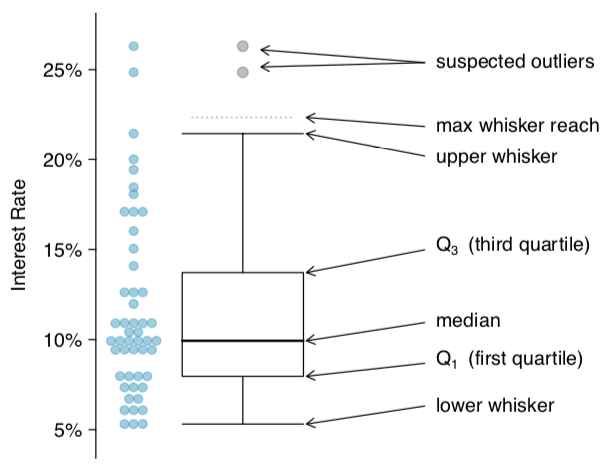
\includegraphics[scale=0.35]{images/boxplot.png}
    \end{center}
\end{frame}

\begin{frame}{Outliers}
    Since we've already built the rest of our boxplot, we can start to think about outliers as whatever is left out. 
    \begin{itemize}
        \item We label these observations specifically because they are \textit{unusual} or \textit{extreme}.
        \item Observations that are unusually far from the rest of the data are referred to as \textbf{outliers}.
    \end{itemize}
\end{frame}

\begin{frame}{Why Examine Outliers?}
    \begin{itemize}
        \item Identify sources of strong skew.
        \item Provide insight into potentially interesting properties of the data.
        \item Identify possible data collection or data entry errors.
    \end{itemize}
\end{frame}

\begin{frame}{Robust Statistics}
    Suppose we have some data:
    \[
    3,  6,  7,  4, 10,  8,  1,  5,  2,  9
    \]
    and I replace the largest observation (10) with a significantly larger value (35).
    \[
    3,  6,  7,  4, 35,  8,  1,  5,  2,  9
    \]
\end{frame}

\begin{frame}{Robust Statistics}
    For our original data,
    \[
    3,  6,  7,  4, 10,  8,  1,  5,  2,  9
    \]
    we get the following:
    \begin{table}[]
        \begin{tabular}{ccccc}
        median & $IQR$ & & $\bar{x}$ & $s$ \\ 
        \hline
        5.5 & 4.5 & & 5.5 & 3.03 
        \end{tabular}
    \end{table}
    
    \vspace{12pt}What do you think will happen to our sample statistics (mean, median, standard deviation, and IQR) when I replace 10 with 35?
\end{frame}

\begin{frame}{Robust Statistics}
    Replacing 10 with 35, these numbers shift somewhat:
    \begin{table}[]
        \begin{tabular}{lccccc}
        & median & $IQR$ & & $\bar{x}$ & $s$ \\ 
        \hline
        Original Data & 5.5 & 4.5 & & 5.5 & 3.03 \\
        Modified Data & 5.5 & 4.5 & & 8.0 & 9.83
        \end{tabular}
    \end{table}
    
    \vspace{12pt}The median and IQR are exactly the same, but the mean and standard deviation change quite a bit!
\end{frame}

\begin{frame}{Robust Statistics}
    We say that the median and IQR are \textbf{robust statistics} or that they are \textit{robust to} outliers, meaning that their values are minimally effected by these extreme observations. 
    \begin{table}[]
        \begin{tabular}{lccccc}
        & \multicolumn{2}{c}{Robust} && \multicolumn{2}{c}{Not Robust} \\
        \hline
        & median & $IQR$ & & $\bar{x}$ & $s$ \\ 
        \hline
        Original Data & 5.5 & 4.5 & & 5.5 & 3.03 \\
        Modified Data & 5.5 & 4.5 & & 8.0 & 9.83
        \end{tabular}
    \end{table}
    
    \vspace{12pt}Why do you think the mean and standard deviation changed so much, but the median and IQR did not?
\end{frame}

\begin{frame}{When Are Robust Statistics Important?}
    \begin{itemize}
        \item Suppose you wanted to know about the typical home price in the United States in 2018.
        \item Recall that the mean and median are both measures of center.
        \item Would you look at the mean or the median? Why?
    \end{itemize}
\end{frame}

\begin{frame}{When Are Robust Statistics Important?}
    As long as you can defend your answer, there is value to each option!
    \begin{itemize}
        \item If we wanted to know what the typical homeowner is spending, the median would be more useful.
        \item If we wanted our estimate to scale, e.g., to estimate how much total money was spent on homes in 2018, the mean might be a better option. 
    \end{itemize}
\end{frame}

\begin{frame}{Transforming Data}
    \begin{itemize}
        \item When data are very strongly skewed, we sometimes transform them to make them easier to model.
        \item For our purposes, data is easiest to model when it is 
        \begin{itemize}
            \item Mostly symmetric
            \item Unimodal
            \item "Bell-shaped"
        \end{itemize}
        \item We want to be able to use our mean and standard deviation instead of our median and IQR!
    \end{itemize}
\end{frame}

\begin{frame}{Transforming Data}
    What does it mean to "transform" the data?
    \begin{itemize}
        \item Essentially, we apply some mathematical function to our data in order to rescale it.
        \item Technically, we want transformations that are continuous and invertible.
        \item Fortunately, there are a number of standard transformations that we use. 
    \end{itemize}
\end{frame}

\begin{frame}{Example: Transforming Data}
    A histogram of the populations of all US counties.
    \begin{center}
        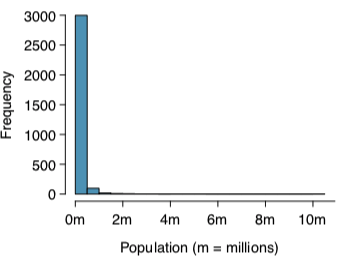
\includegraphics[scale=0.5]{images/trans1.png}
    \end{center}
    For perspective, Riverside County has 2.4 million people and \\ Los Angeles County has 10.2 million people!
\end{frame}

\begin{frame}{Example: Transforming Data}
    \begin{center}
        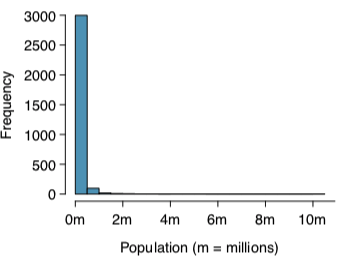
\includegraphics[scale=0.5]{images/trans1.png}
    \end{center}
    
    These data are very strongly skewed! Almost all of the counties have populations between 0 and 1 million people, but a few have over 10 million.
\end{frame}

\begin{frame}{Example: Transforming Data}
    To transform the data we take $\log_{10}(Population)$. The histogram of the transformed data looks like this:
    \begin{center}
        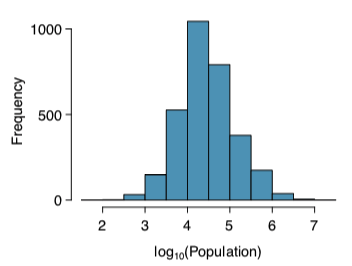
\includegraphics[scale=0.5]{images/trans2.png}
    \end{center}
\end{frame}

\begin{frame}{Example: Transforming Data}
    Before and after transformation:
    \begin{center}
        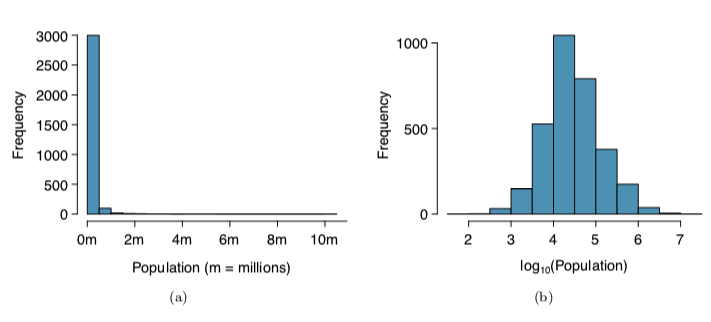
\includegraphics[scale=0.45]{images/transform.png}
    \end{center}
    In histogram (b), it is much more reasonable to use the mean and standard deviation to measure the center and spread of our data.
\end{frame}

\begin{frame}{Transformations}
    We may also apply
    \begin{itemize}
        \item A square root transformation
        \begin{itemize}
            \item $\sqrt{\text{original variable}}$
        \end{itemize}
        \item An inverse transformation
        \begin{itemize}
            \item $(\text{original variable})^{-1}$
        \end{itemize}
    \end{itemize}
\end{frame}

\begin{frame}{Transformations}
    In general, transformations:
    \begin{itemize}
        \item Let us see data structure differently.
        \item Reduce skew.
        \item Assist in modeling.
        \item Straighten nonlinear relationships in scatterplots.
    \end{itemize}
\end{frame}

\begin{frame}{Visualizing Geographic Data}
    \begin{itemize}
        \item Geographic data can be plotted using the data visualization techniques we've already seen.
        \item We might instead want to create an intensity plot.
        \item These plots allow us to show higher and lower values of a variable using colors on a map.
        \item Intensity plots are good for seeing geographic trends.
    \end{itemize}
\end{frame}

\begin{frame}{Mapping Data}
    \begin{center}
        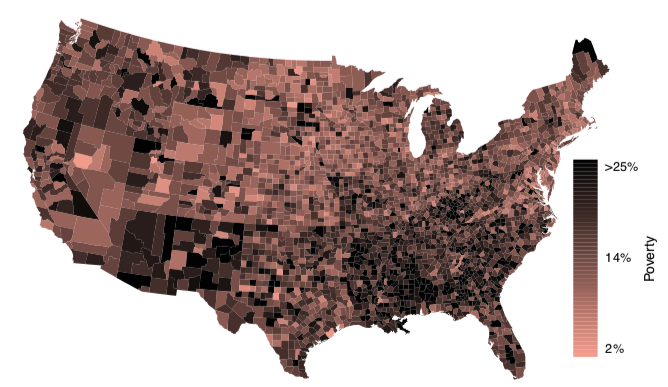
\includegraphics[scale=0.5]{images/map.png}
    \end{center}
\end{frame}


%\input{Sections/s2_1add.tex}
%\section{Section 2.2}
%\begin{frame}{Categorical Data}
    In the previous section, we focused on numerical data. We now turn our attention to categorical data. 
    
    \vspace{24pt}This section includes more tools and language that we will use throughout the course. 
\end{frame}

\begin{frame}{Word Clouds}
    If we have text that we're interested in, we can turn words into categories. Here are the top seven words from the survey question about slaying a dragon:
    
    \begin{center}
        \begin{tabular}{l c}
		    Word    & Frequency \\ \hline
            sword   & 9 \\
            dragon  & 9 \\
            stab    & 6 \\
            kind    & 5 \\
            heart   & 4 \\
            fire    & 3 \\
            dont    & 3 
        \end{tabular}
    \end{center}
\end{frame}

\begin{frame}{Word Clouds}
    Here are a few things I did before finding the top words:
    \begin{itemize}
        \item Removed responses like "N/A" and "I don't know".
        \item Removed low-information words like "the" and "and".
        \item Removed punctuation.
        \item Converted all text to lowercase.
        \item Reduced words to their roots - "kindness" becomes "kind" - to group those words together.
    \end{itemize}
    
    \vspace{12pt}Now we're ready to create a word cloud out of the responses.
\end{frame}

\begin{frame}{Word Clouds}
    \begin{center}
        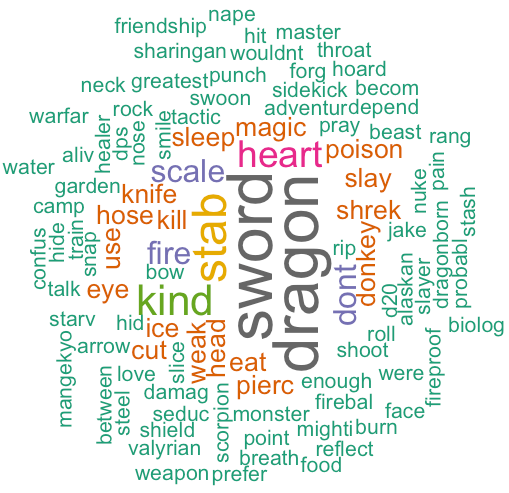
\includegraphics[scale=0.4]{images/dragonCloud.png}
    \end{center}
\end{frame}

\begin{frame}{Summary Tables}
    A basic \textbf{summary table} \textit{summarizes} a categorical variable by showing the frequency, or count, of each category.
    
    \begin{columns}[T] % align columns
        \begin{column}{.48\textwidth}
        %\color{red}\rule{\linewidth}{4pt}
        \begin{center}
        \begin{tabular}{l c}
		    \texttt{homeownership} & Count \\ \hline
		    Rent & 3858 \\ 
		    Mortgage & 4789 \\
		    Own & 1353 \\ \hline
		    Total & 10000 \\ \hline
        \end{tabular}
        \end{center}
        \end{column}%
        \hfill%
        \begin{column}{.48\textwidth}
        %\color{blue}\rule{\linewidth}{4pt}
        \begin{center}
        \begin{tabular}{l c}
		    \texttt{apptype} & Count \\ \hline
		    Individual & 8505 \\ 
		    Joint & 1495 \\ \hline
		    Total & 10000 \\ \hline
        \end{tabular}
        \end{center}
        \end{column}%
    \end{columns}
    \vspace{12pt}Note: \texttt{homeownership} refers to whether or not someone owns a home and \texttt{apptype} indicates whether a loan application was made individually or jointly.
\end{frame}

\begin{frame}{Bar Plots}
    A \textbf{bar plot} is a common way to visualize the information in a summary table. 
    \begin{center}
        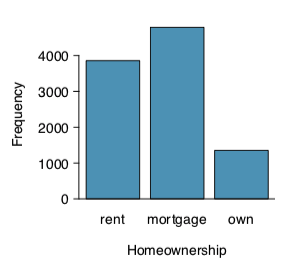
\includegraphics[scale=0.5]{images/barplot_freq.png}
    \end{center}
\end{frame}

\begin{frame}{Summary Tables: Proportions}
    We may occasionally prefer to see our data summarized by proportions (see the fractional breakdown of our data).
    
    \begin{columns}[T] % align columns
        \begin{column}{.48\textwidth}
        %\color{red}\rule{\linewidth}{4pt}
        \begin{center}
        \begin{tabular}{l c}
		    \texttt{homeownership} & Proportion \\ \hline
		    Rent & 0.3858 \\ 
		    Mortgage & 0.4789 \\
		    Own & 0.1353 \\ \hline
		    Total & 1.0000 \\ \hline
        \end{tabular}
        \end{center}
        \end{column}%
        \hfill%
        \begin{column}{.48\textwidth}
        %\color{blue}\rule{\linewidth}{4pt}
        \begin{center}
        \begin{tabular}{l c}
		    \texttt{apptype} & Proportion \\ \hline
		    Individual & 0.8505 \\ 
		    Joint & 0.1495 \\ \hline
		    Total & 1.0000 \\ \hline
        \end{tabular}
        \end{center}
        \end{column}%
    \end{columns}
\end{frame}

\begin{frame}{Bar Plots}
    We can again use a bar plot to visualize this information.
    \begin{center}
        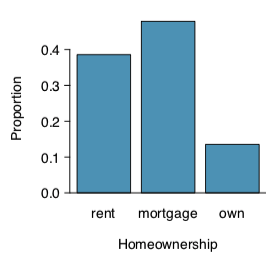
\includegraphics[scale=0.5]{images/barplot_prop.png}
    \end{center}
    This bar plot looks exactly the same as the one with frequencies! The only difference is in the numbers along the vertical axis.
\end{frame}

\begin{frame}{Pie Charts}
    Pie charts show the same information as bar charts, but are more difficult to discern details from. 
    \begin{center}
        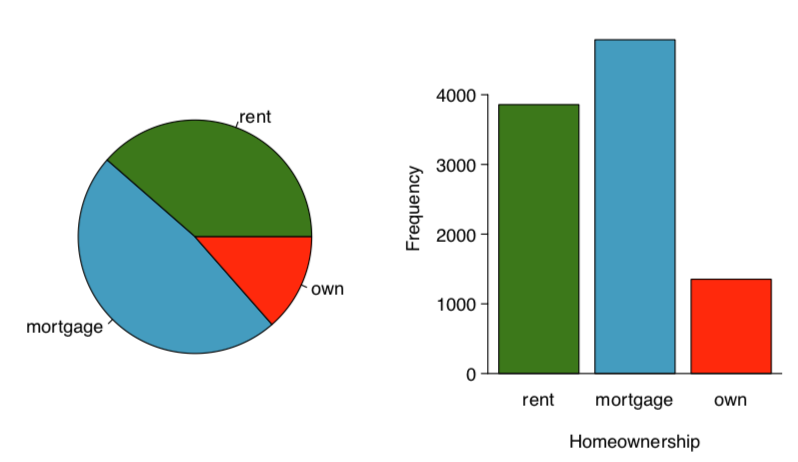
\includegraphics[scale=0.3]{images/piechart.png}
    \end{center}
    They are good for infographics but are not well-suited to technical writing.
\end{frame}

\begin{frame}{Contingency Tables}
    A \textbf{contingency table} is a table that summarizes two categorical variables. It looks something like this:
    \begin{center}
        \begin{tabular}{r l ccc r}
		& & \multicolumn{3}{c}{{\texttt{homeownership}}} & \\
        \cline{3-5}
		& & Rent & Mortgage & Own & Total  \\ 
        \cline{2-6}
        \multirow{2}{*}{{\texttt{apptype}}} 
        & Individual & 3496 & 3839 & 1170 & 8505 \\ 
  		& Joint & 362 & 950 & 183 & 1495 \\ 
        \cline{2-6}
  		& Total	& 3858 & 4789 & 1353 & 10000 \\
        \cline{2-6}
    \end{tabular}
    \end{center}
\end{frame}

\begin{frame}{Contingency Tables}
    \vspace{12pt}Contingency tables allow us to summarize two categorical variables together by breaking them down into subcategories. 
    \begin{center}
        \begin{tabular}{r l ccc r}
		& & \multicolumn{3}{c}{{\texttt{homeownership}}} & \\
        \cline{3-5}
		& & Rent & Mortgage & Own & Total  \\ 
        \cline{2-6}
        \multirow{2}{*}{{\texttt{apptype}}} 
        & Individual & 3496 & 3839 & 1170 & 8505 \\ 
  		& Joint & 362 & 950 & 183 & 1495 \\ 
        \cline{2-6}
  		& Total	& 3858 & 4789 & 1353 & 10000 \\
        \cline{2-6}
    \end{tabular}
    \end{center}
\end{frame}

\begin{frame}{Contingency Tables}
    Notice that the column of totals is the same as the summary table for \texttt{apptype} and the row of totals has the same information as the summary table for \texttt{homeownership}. 
    \begin{center}
        \begin{tabular}{r l ccc r}
		& & \multicolumn{3}{c}{{\texttt{homeownership}}} & \\
        \cline{3-5}
		& & Rent & Mortgage & Own & Total  \\ 
        \cline{2-6}
        \multirow{2}{*}{{\texttt{apptype}}} 
        & Individual & 3496 & 3839 & 1170 & 8505 \\ 
  		& Joint & 362 & 950 & 183 & 1495 \\ 
        \cline{2-6}
  		& Total	& 3858 & 4789 & 1353 & 10000 \\
        \cline{2-6}
    \end{tabular}
    \end{center}
\end{frame}

\begin{frame}{Row and Column Proportions}
    We may also want to examine the fractional breakdown of our contingency table data.
    \begin{itemize}
        \item \textbf{The row proportions are the row counts divided by the row total}.
        \item The column proportions are the column counts divided by the column total.
        \item The overall proportions are the counts divided by the total number of observations. 
    \end{itemize}
\end{frame}

\begin{frame}{Contingency Tables for Row Proportions}
    We can now convert our previous contingency table into a contingency table \textit{for the row proportions}:
    \begin{center}
        \begin{tabular}{r l ccc r}
		& & \multicolumn{3}{c}{{\texttt{homeownership}}} & \\
        \cline{3-5}
		& & Rent & Mortgage & Own & Total  \\ 
        \cline{2-6}
        \multirow{2}{*}{{\texttt{apptype}}} 
        & Individual & 0.411 & 0.451 & 0.138 & 1.000 \\ 
  		& Joint & 0.242 & 0.635 & 0.122 & 1.000 \\ 
        \cline{2-6}
  		& Total	& 0.386 & 0.479 & 0.135 & 1.000 \\
        \cline{2-6}
    \end{tabular}
    \end{center}
    
    \vspace{12pt}This breaks down each application type into home ownership status. We would say that, \textit{among individual applications}, 41.1\% are renters. 
\end{frame}

\begin{frame}{Contingency Tables for Row Proportions}
    \begin{center}
        \begin{tabular}{r l ccc r}
		& & \multicolumn{3}{c}{{\texttt{homeownership}}} & \\
        \cline{3-5}
		& & Rent & Mortgage & Own & Total  \\ 
        \cline{2-6}
        \multirow{2}{*}{{\texttt{apptype}}} 
        & Individual & 0.411 & 0.451 & 0.138 & 1.000 \\ 
  		& Joint & 0.242 & 0.635 & 0.122 & 1.000 \\ 
        \cline{2-6}
  		& Total	& 0.386 & 0.479 & 0.135 & 1.000 \\
        \cline{2-6}
    \end{tabular}
    \end{center}
    We can tell at a glance that this is for the \textit{row proportions} because all of the \textit{row totals} are 1. 
    
    \vspace{12pt}The rows are total breakdown of \texttt{homeownership}, so the bottom row of totals is the same as the home ownership summary table with proportions (see slide 15). They are \textit{not} the additive total for the row of proportions.
\end{frame}

\begin{frame}{Row and Column Proportions}
    \begin{itemize}
        \item The row proportions are the row counts divided by the row total.
        \item \textbf{The column proportions are the column counts divided by the column total}.
        \item The overall proportions are the counts divided by the total number of observations. 
    \end{itemize}
\end{frame}

\begin{frame}{Contingency Tables for Column Proportions}
    We can also convert our contingency table into a contingency table \textit{for the column proportions}:
    \begin{center}
        \begin{tabular}{r l ccc r}
		& & \multicolumn{3}{c}{{\texttt{homeownership}}} & \\
        \cline{3-5}
		& & Rent & Mortgage & Own & Total  \\ 
        \cline{2-6}
        \multirow{2}{*}{{\texttt{apptype}}} 
        & Individual & 0.906 & 0.802 & 0.865 & 0.851 \\ 
  		& Joint & 0.094 & 0.198 & 0.135 & 0.150 \\ 
        \cline{2-6}
  		& Total	& 1.000 & 1.000 & 1.000 & 1.000 \\
        \cline{2-6}
    \end{tabular}
    \end{center}
    
    \vspace{12pt}This breaks down each home ownership status into application types. We would say that, \textit{among renters}, 90.6\% filled out an individual loan application. 
\end{frame}

\begin{frame}{Contingency Tables for Row Proportions}
    \begin{center}
        \begin{tabular}{r l ccc r}
		& & \multicolumn{3}{c}{{\texttt{homeownership}}} & \\
        \cline{3-5}
		& & Rent & Mortgage & Own & Total  \\ 
        \cline{2-6}
        \multirow{2}{*}{{\texttt{apptype}}} 
        & Individual & 0.906 & 0.802 & 0.865 & 0.851 \\ 
  		& Joint & 0.094 & 0.198 & 0.135 & 0.150 \\ 
        \cline{2-6}
  		& Total	& 1.000 & 1.000 & 1.000 & 1.000 \\
        \cline{2-6}
    \end{tabular}
    \end{center}
    We can tell at a glance that this is for the \textit{column proportions} because all of the \textit{column totals} are 1. 
    
    \vspace{12pt}The rows are the total breakdown of \texttt{apptype}, so the bottom row of totals is the same as the application type ownership summary table with proportions (see slide 15). They are \textit{not} the additive total for the column of proportions. 
\end{frame}

\begin{frame}{Contingency Tables for Row Proportions}
    \begin{center}
        \begin{tabular}{l ccc r}
		& Rent & Mortgage & Own & Total  \\ 
        \cline{2-5}
        Individual & 0.906 & 0.802 & 0.865 & 0.851 \\ 
  		Joint & 0.094 & 0.198 & 0.135 & 0.150 \\ 
        \cline{2-5}
  		Total	& 1.000 & 1.000 & 1.000 & 1.000 \\
        \cline{2-5}
    \end{tabular}
    \end{center}
    \begin{itemize}
        \item We can use these contingency tables to check for an association between home ownership and loan type.
        \item Notice that, among individual applicants, 90.5\% rent, but only 80.2\% have a mortgage.
    \end{itemize}
\end{frame}

\begin{frame}{Contingency Tables for Row Proportions}
    \begin{center}
        \begin{tabular}{l ccc r}
		& Rent & Mortgage & Own & Total  \\ 
        \cline{2-5}
        Individual & 0.906 & 0.802 & 0.865 & 0.851 \\ 
  		Joint & 0.094 & 0.198 & 0.135 & 0.150 \\ 
        \cline{2-5}
  		Total	& 1.000 & 1.000 & 1.000 & 1.000 \\
        \cline{2-5}
    \end{tabular}
    \end{center}
    \begin{itemize}
        \item If there is no association, the proportions will be (approximately) the same across the row.
        \item We say that loan types \textit{vary between} different \textbf{levels} of home ownership. 
        \item (Using the column proportions, we can also say that home ownership status varies between levels of loan type.)
    \end{itemize}
\end{frame}

\begin{frame}{Example: Student Survey}
    Let's look at a contingency table for some of our survey data.
    
    \begin{center}
        \begin{tabular}{r l cccc r}
		& & \multicolumn{4}{c}{{\texttt{Year}}} & \\
        \cline{3-6}
		& & Sophomore & Junior & Senior & Other & Total  \\ 
        \cline{2-7}
        \multirow{2}{*}{{\texttt{Want}}} 
        & 1 & 1 & 0 & 2 & 1 & 4 \\ 
  		& 2 & 0 & 4 & 3 & 1 & 8 \\ 
  		& 3 & 1 & 11 & 1 & 0 & 23 \\ 
  		& 4 & 7 & 10 & 8 & 1 & 26 \\ 
  		& 5 & 0 & 3 & 1 & 0 & 4 \\ 
        \cline{2-7}
  		& Total	& 9 & 28 & 25 & 3 & 65 \\
        \cline{2-7}
    \end{tabular}
    \end{center}
    
    Is there a relationship between year and desire to take this course?
\end{frame}

\begin{frame}{Example: Student Survey}
    It's hard to tell! Let's look at whether there is a change in \texttt{want} by \texttt{year} (does want vary between levels of year).
    
    \begin{center}
        \begin{tabular}{r l cccc r}
		& & \multicolumn{4}{c}{{\texttt{Year}}} & \\
        \cline{3-6}
		& & Sophomore & Junior & Senior & Other & Total  \\ 
        \cline{2-7}
        \multirow{2}{*}{{\texttt{Want}}} 
        & 1 & 0.11 & 0.00 & 0.08 & 0.33 & 0.06 \\ 
  		& 2 & 0.00 & 0.14 & 0.12 & 0.33 & 0.12 \\ 
  		& 3 & 0.11 & 0.39 & 0.44 & 0.00 & 0.35 \\ 
  		& 4 & 0.78 & 0.36 & 0.32 & 0.33 & 0.40 \\ 
  		& 5 & 0.00 & 0.11 & 0.04 & 0.00 & 0.06 \\ 
        \cline{2-7}
  		& Total	& 1.00 & 1.00 & 1.00 & 1.00 & 1.00 \\
        \cline{2-7}
    \end{tabular}
    \end{center}
    
    Is there a relationship between year and desire to take this course?
\end{frame}

\begin{frame}{Example: Student Survey}
    What if we looked at whether there is a change in \texttt{year} by \texttt{want} (does year vary between levels of want)?
    \begin{itemize}
        \item We should still see a relationship.
        \item It makes sense to think about whether year affects your desire to take this course.
        \item However, it probably doesn't make sense to think about whether desire to take this course affects your year in school.
        \begin{itemize}
            \item In this scenario, you'd have to have done something extreme like taken a year off and fallen behind just because you really didn't want to take this course. Hopefully that's not the case!
        \end{itemize}
    \end{itemize}
\end{frame}

\begin{frame}{Two-Variable Bar Plots}
    \begin{itemize}
        \item We can extend our bar plots to help visualize the information in a contingency table by creating
        \begin{itemize}
            \item \textbf{Stacked bar plots}.
            \item \textbf{Side-by-side bar plots}.
        \end{itemize} 
        \item A stacked bar plot takes our one-variable bar plot and breaks up the bars to show a second variable.
        \item A side-by-side bar plot takes our one-variable var plot and splits each bar into two side-by-side bars.
    \end{itemize}
\end{frame}

\begin{frame}{Side-By-Side Bar Plots}
    \begin{center}
        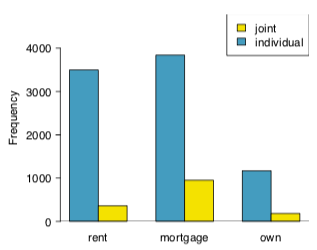
\includegraphics[scale=0.45]{images/sidebar.png}
    \end{center}
    This side-by-side bar plot shows home ownership with loan application type. Here, we're breaking the data into six categories and giving each one a bar.
\end{frame}

\begin{frame}{Stacked Bar Plots}
    \begin{center}
        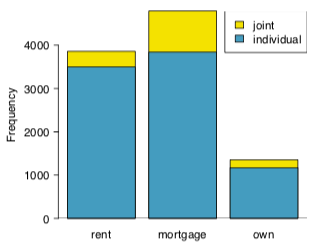
\includegraphics[scale=0.45]{images/stackedbar.png}
    \end{center}
    This stacked bar plot shows home ownership broken down by loan application type. 
    
    \vspace{12pt}In both plots, it is easy to see that there are fewer people who own their homes and fewer people applying for joint loans. 
\end{frame}

\begin{frame}{Stacked Bar Plots: Frequencies}
    \begin{center}
        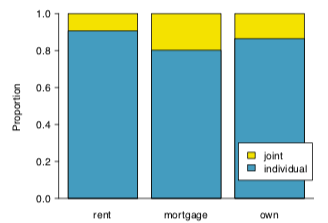
\includegraphics[scale=0.45]{images/stackedbarstd.png}
    \end{center}
    \begin{itemize}
        \item Same information, but standardized based on home ownership.
        \item This is a visualization of the frequency-based contingency table for loan types varying between levels of home ownership (slide 30). 
        \item Now we can see that the two variables are associated.
    \end{itemize}
\end{frame}

\begin{frame}{Example: Student Survey Data}
    Let's turn our contingency table into a stacked bar plot:
    \begin{center}
        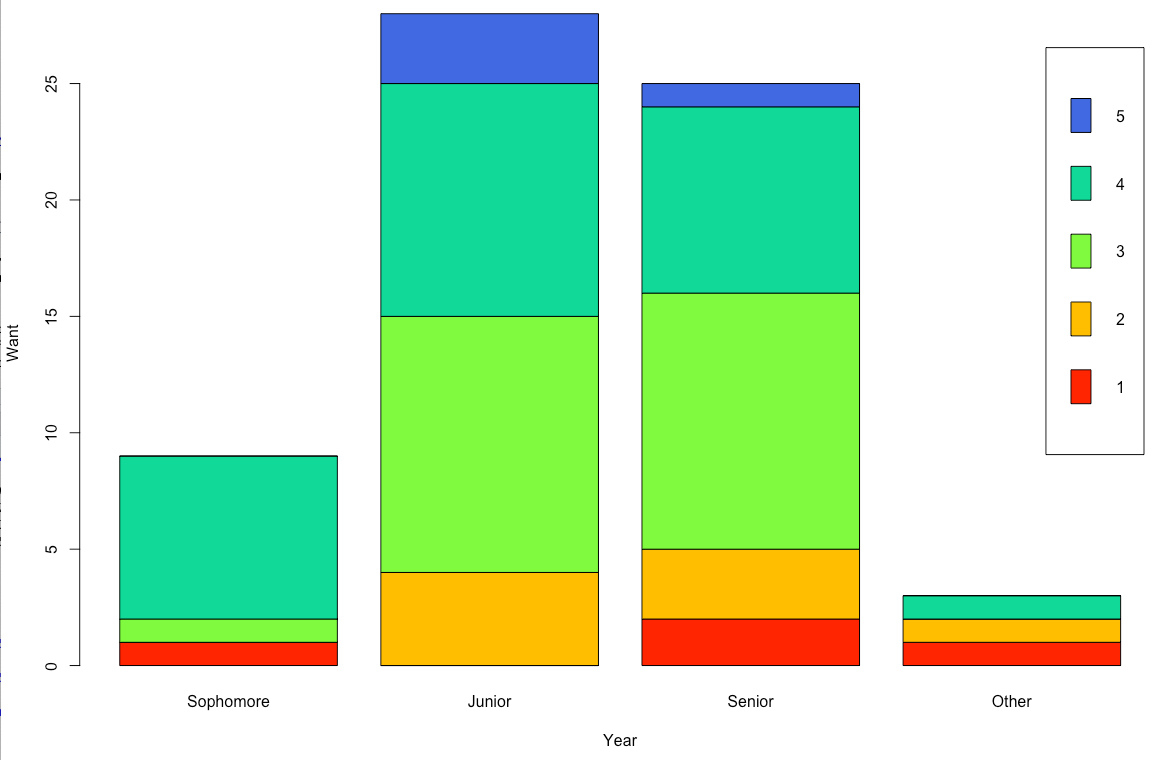
\includegraphics[scale=0.18]{images/exbarplot.png}
    \end{center}
    Here, we can see that most of you are juniors and seniors (and that there's a decent spread of how much you want to be here).
\end{frame}

\begin{frame}{Example: Student Survey Data}
    Let's do the same with the proportion-based table:
    \begin{center}
        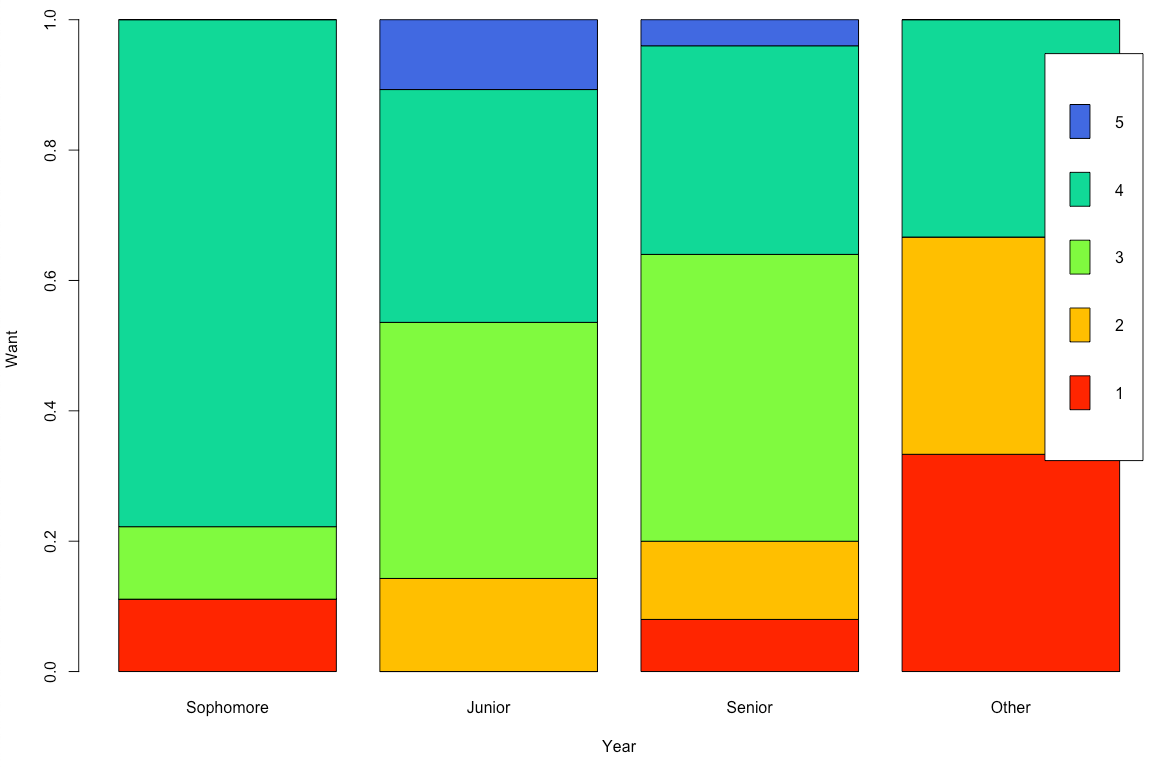
\includegraphics[scale=0.2]{images/exbarplot2.png}
    \end{center}
    Now we can quickly visualize the differences between the years.
\end{frame}

\begin{frame}{Mosaic Plots}
    \begin{center}
        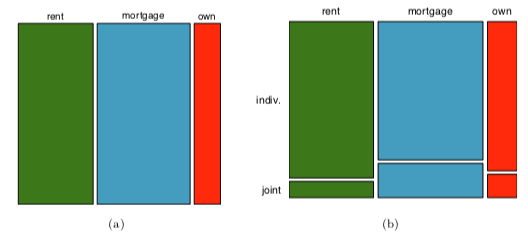
\includegraphics[scale=0.5]{images/mosaic.png}
    \end{center}
    \noindent(a) is a one-variable mosaic plot for \texttt{homeownership}.\\
    \noindent(b) is a two-variable mosaic plot for \texttt{homeownership} and \texttt{app\_type}.
\end{frame}

\begin{frame}{Mosaic Plots}
    \begin{itemize}
        \item Mosaic plots look a lot like bar plots, but now the \textit{widths} of the bars depend on the group sizes.
        \item For two-variable mosaic plots, the boxes from the one-variable mosaic plot are divided up using the second variable.
        \item Now, the \textit{heights} of the boxes also depend on group sizes.
        \item Thus, mosaic plots use \textit{area} to represent the number of cases in each category.
    \end{itemize}
\end{frame}

\begin{frame}{Example: Student Survey Data}
    \begin{center}
        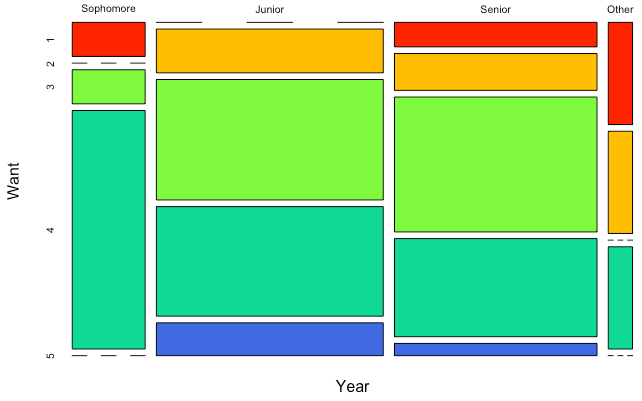
\includegraphics[scale=0.35]{images/mosaicex.png}
    \end{center}
    We can again see that there are more juniors \& seniors in the class and that sophomores are more likely to want to take this course beyond its being a requirement. 
\end{frame}

\begin{frame}{Comparing Numerical Data Across Groups}
    \begin{itemize}
        \item Our question of interest often involves comparing numerical data across categories.
        \item Whenever we are interested in comparing some numeric outcome across treatment groups, this is our goal!
        \item In general, these comparisons require that we make side-by-side or stacked versions of our data visualization techniques for numerical data.
    \end{itemize}
\end{frame}

\begin{frame}{Side-By-Side Box Plots}
    \textbf{Side-by-side box plots} are standard tools for visualizing numerical data broken down into categories.
    
    \begin{center}
        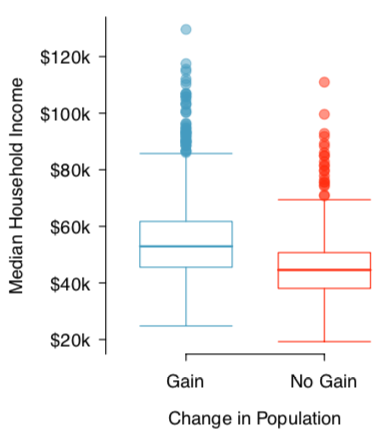
\includegraphics[scale=0.35]{images/sidesidebox.png}
    \end{center}
\end{frame}

\begin{frame}{Example: Student Survey Data}
    Let's look at how number of pets differs between year: 
    \begin{center}
        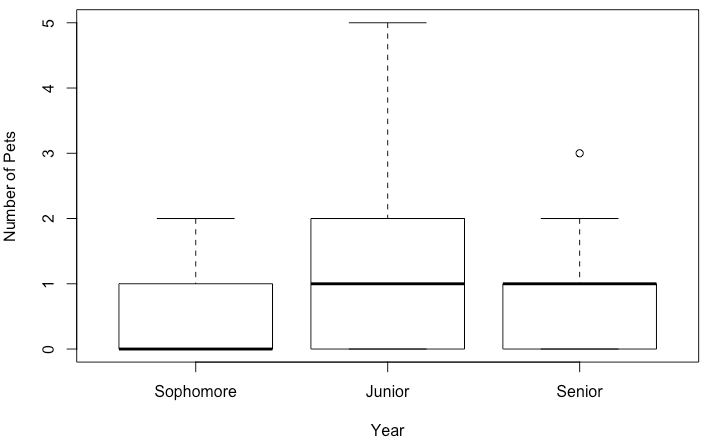
\includegraphics[scale=0.3]{images/petsyearbox.png}
    \end{center}
    Juniors have a larger IQR and longer whiskers, suggesting that they have a larger spread in number of pets.
\end{frame}

\begin{frame}{Hollow (or Stacked) Histograms}
    \begin{center}
        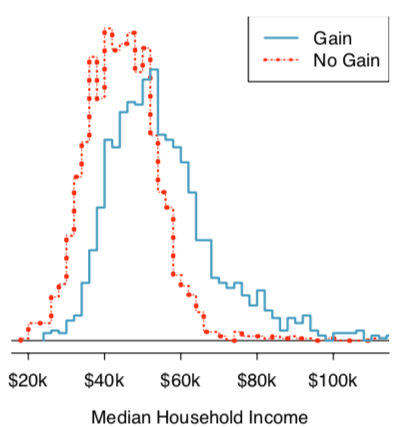
\includegraphics[scale=0.33]{images/hollowhists.png}
    \end{center}
    Hollow histograms are a little bit harder to read, but they allow us to visualize what two distributions look like when layered on top of each other.
\end{frame}

%\section{Section 2.3}
%\begin{frame}{Case Study}
    \begin{itemize}
        \item Suppose we split the class into two groups by drawing a line down the middle of the classroom.
        \item Let $\hat{p}_L$ be the proportion of students on the left side who own an Apple product.
        \item Let $\hat{p}_R$ be the proportion of students on the right side who own an Apple product.
    \end{itemize}
    Would you expect these two proportions to be \textit{exactly} the same?
\end{frame}

\begin{frame}{Case Study}
    \begin{itemize}
        \item There's no reason to believe that Apple users tend to sit on one side of the room or another*, so we would expect the proportions to be pretty similar.
        \item But we probably wouldn't expect these numbers to be exactly the same.
        \item This small expected variation is due to random chance.
    \end{itemize}
    
    \vspace{12pt}* What assumption are we making about how these variables relate to one another?
\end{frame}

\begin{frame}{Case Study: Malaria Vaccine}
    We consider a study on the malaria vaccine, PfSPZ. 
    \begin{itemize}
        \item Volunteer patients randomized into one of two experimental groups.
        \begin{itemize}
            \item 14 patients received the vaccine.
            \item 6 patients recieved a placebo.
        \end{itemize}
        \item After 19 weeks, all patients are exposed to a (drug-sensitive) strain of malaria.
    \end{itemize}
\end{frame}

\begin{frame}{Case Study: Malaria Vaccine}
    These are the results:
    \begin{center}
        \begin{tabular}{r l cc r}
		& & \multicolumn{2}{c}{{\texttt{outcome}}} & \\
        \cline{3-5}
		& & Infection & No Infection & Total  \\ 
        \cline{2-5}
        \multirow{2}{*}{{\texttt{treatment}}} 
        & Vaccine & 5 & 9 & 14  \\ 
  		& Placebo & 6 & 0 & 6  \\ 
        \cline{2-5}
  		& Total	& 11 & 9 & 20  \\
        \cline{2-5}
    \end{tabular}
    \end{center}
    This suggests infection rates of 35.7\% for the treatment group and 100\% for the control (placebo) group.
\end{frame}

\begin{frame}{Case Study: Malaria Vaccine}
    \begin{itemize}
        \item This study is an experiment, because treatment levels were assigned by the researchers.
        \item Therefore we can evaluate a causal relationship between the vaccine and incidence of malaria.
        \item It is not clear what level of blinding was used, but since they used a placebo, it is probably blind.
    \end{itemize}
\end{frame}

\begin{frame}{Strength of Evidence}
    \begin{itemize}
        \item We expect there to be some differences in our sample estimates, even if the true values are exactly equal. 
        \item The sample size is small, so it's not clear whether the vaccine would be effective in the population at large.
        \item It's impossible to know whether the observed difference is due to the vaccine's efficacy or random chance.
        \item It's possible that such a large difference is normal (due to chance alone) in such a small sample.
    \end{itemize}
    \vspace{12pt}\small Note: In reality, clinical trials suggest that PfSPZ is effective, but storage and transportation costs make it difficult to distribute to areas where malaria is prevalent.
\end{frame}

\begin{frame}{Variability in the Data}
    This is a good reminder that our observed data may not perfectly reflect the truth!
    \begin{itemize}
        \item This is due to \textbf{random noise}, the variability between values due to random chance.
        \item Random noise and sample size are things we take into account when statistically analyzing scientific claims.
    \end{itemize}
\end{frame}

\begin{frame}{Competing Claims}
    Whenever we ask a research question, we always have two competing claims, or \textbf{hypotheses}. These are labeled $H_0$ ("H-nought") and $H_A$ ("H-A").
    
    \vspace{12pt}$H_0$: \textbf{Independence model}. The variables treatment and outcome are independent. They have no relationship. Any observed difference between the proportion of patients who developed an infection in the two groups is due to chance.
    
    \vspace{12pt}$H_A$: \textbf{Alternative model}. The variables are not independent. The difference in infection rates is not due to chance. The vaccine affected the rate of infection.
\end{frame}

\begin{frame}{Independence Model}
    If $H_0$, the independence model, is true
    \begin{itemize}
        \item The vaccine is irrelevant to infection status.
        \item The 11 patients who developed an infection would have develop an infection regardless of which group they were assigned to.
        \item The 9 who did not develop an infection wouldn't have developed an infection regardless of which group they were assigned to.
        \item The difference in infection rates was due to chance alone.
    \end{itemize}
\end{frame}

\begin{frame}{Alternative Model}
    If $H_A$, the alternative model, is true
    \begin{itemize}
        \item Infection rates are influenced by whether or not a person received the vaccine.
    \end{itemize}
\end{frame}

\begin{frame}{Which Model is Correct?}
    We draw conclusions about which model is more likely to be true by assessing how strong our evidence is
    \begin{itemize}
        \item Do the data conflict with $H_0$ strongly enough to conclude $H_A$?
        \item This depends on
        \begin{enumerate}
            \item How different the groups are.
            \item How variable the groups are.
            \item How much data we have.
        \end{enumerate}
    \end{itemize}
\end{frame}

\begin{frame}{Simulations}
    We can start to think about the strength of our evidence using simulations.
    \begin{itemize}
        \item Our simulations will assume that our independence model is true.
        \item We want to know if it is common to see differences as large as the one we saw in our study.
        \item If it is common, it is more likely that the difference was due to random chance.
        \item If it is uncommon, it is more likely that the vaccine is helpful in preventing malaria.
    \end{itemize}
\end{frame}

\begin{frame}{Simulations}
    Simulations sound complicated, but the idea here is just to assume that the vaccine has no effect and then re-randomize the patients to the treatment and control groups.
    \begin{itemize}
        \item If the vaccine has no effect, we assume that the 11 patients who developed an infection would have done so no matter what. 
        \item We also assume that the 9 who did not develop an infection would have no infection no matter what.
    \end{itemize}
\end{frame}

\begin{frame}{Simulations}
    We can approach this simulation like this:
    \begin{enumerate}
        \item Take 20 note cards to represent the 20 patients \item Write each infection status on a note card (11 will say "infection"; 9 will say "no infection").
        \item Shuffle the note cards and then randomly pull out 14 for the \texttt{vaccine} pile. Put the other 6 into the \texttt{placebo} pile.
        \item Count up how many infections are in each pile.
    \end{enumerate}
\end{frame}

\begin{frame}{Simulations}
    Doing this once, we get
    \begin{center}
        \begin{tabular}{r l cc r}
		& & \multicolumn{2}{c}{{\texttt{outcome}}} & \\
        \cline{3-5}
		& & Infection & No Infection & Total  \\ 
        \cline{2-5}
        \multirow{2}{*}{{\texttt{treatment}}} 
        & Vaccine & 7 & 7 & 14  \\ 
  		& Placebo & 4 & 2 & 6  \\ 
        \cline{2-5}
  		& Total	& 11 & 9 & 20  \\
        \cline{2-5}
    \end{tabular}
    \end{center}
    Here, there is an infection rate of 50\% for the treatment group and 66.6\% in the placebo group, a difference of 16.7\%. This is much smaller than in the actual study!
\end{frame}

\begin{frame}{Checking For Independence}
    The real power of simulations comes from repetition. Using \texttt{R}, I repeated this simulation 10,000 times. 
    \begin{center}
        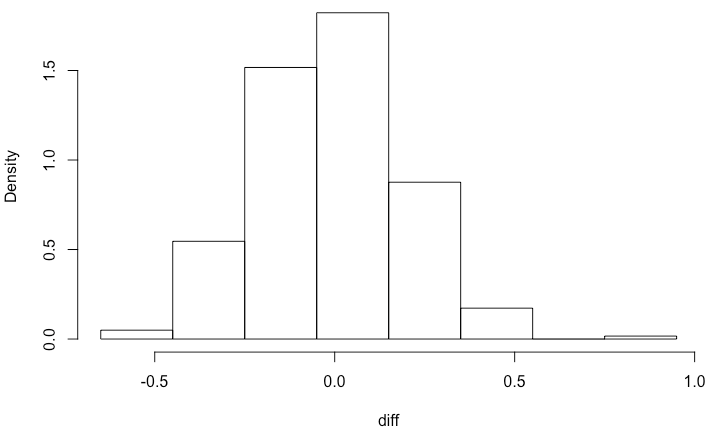
\includegraphics[scale=0.3]{images/diffhist.png}
    \end{center}
    Histogram of the differences across 10,000 repetitions.
\end{frame}

\begin{frame}{Checking For Independence}
    \begin{itemize}
        \item In the actual study, the difference in infection rates was 64.3\%.
        \item In my simulations, the average difference was only 0.06\%.
        \item I found a difference as big as the one in the study only 33 times.
        \begin{itemize}
            \item This means that, if the vaccine is not useful, a difference of 64.3\% happens by chance less than 1\% of the time!
        \end{itemize}
        \item This suggests that we have pretty good information despite the small sample size.
    \end{itemize}
\end{frame}

\begin{frame}{Moving Forward}
    The concepts we've been talking about with our case study are what we want to get at with this course!
    \begin{itemize}
        \item Hypotheses
        \item Testing claims (testing for independence)
        \item Figuring out how uncertain we are about our results
    \end{itemize}
    Eventually, we will formalize these concepts and talk about how to test our claims without simulations.
\end{frame}

\begin{frame}{A Note About R Code}
    I've been using a lot of code to write these slides!
    \begin{itemize}
        \item I've added a new page to the course website that will contain links to all of this R code.
        \item This code will be heavily commented to make it easier to follow and I will set it up so that you will not need to download any additional data.
        \item As always, learning R is completely optional, but the code is there if you're interested.
    \end{itemize}
\end{frame}

%\section{Section 3.1}
%\begin{frame}{Probability}
    When we talked about the small sample malaria experiment, what we really wanted to know was, if the independence model is correct, what is the \textit{probability} that we'd see a difference as large as 64.3\%?
    \begin{itemize}
        \item Probability forms the foundation of statistics.
        \item You already know about a lot of these ideas!
        \begin{itemize}
            \item You may not have thought about them much, but you deal with probability automatically all the time. 
        \end{itemize}
        \item We are going to formalize these concepts.
    \end{itemize}
\end{frame}

\begin{frame}{Example: Rolling a Die}
    If you play any kind of dice-based tabletop games, you are probably familiar with weighing your options before making your next roll. This the kind of probability concept we want to formalize!
    
    \vspace{12pt}Suppose we have a six-sided die (d6). If we roll our d6 one time, what are the chances that we roll a \texttt{1}?
\end{frame}

\begin{frame}{Example: Rolling a Die}
    \begin{itemize}
        \item We assume that our d6 is a fair die, so it's not weighted toward any number in particular. 
        \item This means that all 6 numbers are equally likely.
        \item Therefore there is a 1-out-of-6 chance that we roll that \texttt{1}.
        \item When talking about probability, we write 1-out-of-6 as a fraction or decimal: $1/6 = 0.167$.
        \item We might also say that we have a 16.7\% chance of rolling a \texttt{1}.
    \end{itemize}
\end{frame}

\begin{frame}{Example 2: Rolling a Die}
    Suppose we need to roll at least a \texttt{4} to succeed in some game move. What are the chances that we succeed?
\end{frame}

\begin{frame}{Example 2: Rolling a Die}
    Suppose we need to roll at least a \texttt{4} to succeed in some game move. What are the chances that we succeed?
    \begin{itemize}
        \item To succeed, we can roll a \texttt{4}, \texttt{5}, or \texttt{6}.
        \item Our d6 has 6 sides and there are 3 numbers that result in success.
        \item Thus there is a 3-out-of-6 chance that we succeed, or $3/6 = 1/2 = 0.5$, a 50\% chance.
    \end{itemize}
\end{frame}

\begin{frame}{Example 3: Rolling a Die}
    What if we are interested in rolling a \texttt{1}, \texttt{2}, \texttt{3}, \texttt{4}, \texttt{5}, or \texttt{6}?
\end{frame}

\begin{frame}{Example 3: Rolling a Die}
    What if we are interested in rolling a \texttt{1}, \texttt{2}, \texttt{3}, \texttt{4}, \texttt{5}, or \texttt{6}?
    \begin{itemize}
        \item This is all of the possible sides.
        \item We have to roll at least one of those numbers (we cannot fail to roll a \texttt{1}, \texttt{2}, \texttt{3}, \texttt{4}, \texttt{5}, \textit{or} \texttt{6}).
        \item There is a 6-out-of-6 chance that we roll one of these numbers, or $6/6=1$ a 100\% chance.
    \end{itemize}
\end{frame}

\begin{frame}{Example 4: Rolling a Die}
    What if we are happy as long as we do \textbf{not} roll a \texttt{1}?
\end{frame}

\begin{frame}{Example 4: Rolling a Die}
    What if we are happy as long as we do \textbf{not} roll a 1?
    \begin{itemize}
        \item The chances of rolling a \texttt{1}, \texttt{2}, \texttt{3}, \texttt{4}, \texttt{5}, or \texttt{6} are 100\%.
        \item The chances of rolling a \texttt{1} are 16.7\%.
        \item So the chances of rolling a \texttt{2}, \texttt{3}, \texttt{4}, \texttt{5} , or \texttt{6} (but not a \texttt{1}) are $100\% - 16.7\% = 83.3\%$
    \end{itemize}
\end{frame}

\begin{frame}{Example 4: Rolling a Die}
    What if we are happy as long as we do \textbf{not} roll a \texttt{1}?
    \begin{itemize}
        \item Alternately, we can calculate this directly: not rolling a \texttt{1} means rolling a \texttt{2}, \texttt{3}, \texttt{4}, \texttt{5}, or \texttt{6}.
        \item The chances of rolling a \texttt{2}, \texttt{3}, \texttt{4}, \texttt{5}, or \texttt{6} are 5-out-of-6, or $5/6=0.833$, 83.3\%.
    \end{itemize}
\end{frame}

\begin{frame}{Example 5: Rolling a Die}
    What if we have 2d6? What is the chance that we roll two \texttt{1}s?
\end{frame}

\begin{frame}{Example 5: Rolling a Die}
    What if we have 2d6? What is the chance that we roll two \texttt{1}s?
    \begin{itemize}
        \item We know that there is a 1/6 chance that the first die is a \texttt{1}.
        \item Then, \textit{of those 1/6 times}, there is a 1/6 chance that the second die is a \texttt{1}.
        \item Then the chance that both dice roll a \texttt{1} is $(1/6)\times(1/6)=1/36$ or 2.78\%.
    \end{itemize}
\end{frame}

\begin{frame}{Example 5: Rolling a Die}
    We can also picture this in a table:
    \begin{table}[]
    \begin{tabular}{rccccccc}
    \multicolumn{1}{c}{}                                  &                        & \multicolumn{6}{c}{\texttt{first die}}                                                                                       \\
    \multicolumn{1}{c}{}                                  &                        & 1                     & 2                     & 3                     & 4                     & 5                     & 6                     \\ \cline{3-8} 
    \multirow{6}{*}{\texttt{second die}} & \multicolumn{1}{c|}{1} & \multicolumn{1}{c|}{\texttt{X}} & \multicolumn{1}{c|}{} & \multicolumn{1}{c|}{} & \multicolumn{1}{c|}{} & \multicolumn{1}{c|}{} & \multicolumn{1}{c|}{} \\ \cline{3-8} 
                                                      & \multicolumn{1}{c|}{2} & \multicolumn{1}{c|}{} & \multicolumn{1}{c|}{} & \multicolumn{1}{c|}{} & \multicolumn{1}{c|}{} & \multicolumn{1}{c|}{} & \multicolumn{1}{c|}{} \\ \cline{3-8} 
                                                      & \multicolumn{1}{c|}{3} & \multicolumn{1}{c|}{} & \multicolumn{1}{c|}{} & \multicolumn{1}{c|}{} & \multicolumn{1}{c|}{} & \multicolumn{1}{c|}{} & \multicolumn{1}{c|}{} \\ \cline{3-8} 
                                                      & \multicolumn{1}{c|}{4} & \multicolumn{1}{c|}{} & \multicolumn{1}{c|}{} & \multicolumn{1}{c|}{} & \multicolumn{1}{c|}{} & \multicolumn{1}{c|}{} & \multicolumn{1}{c|}{} \\ \cline{3-8} 
                                                      & \multicolumn{1}{c|}{5} & \multicolumn{1}{c|}{} & \multicolumn{1}{c|}{} & \multicolumn{1}{c|}{} & \multicolumn{1}{c|}{} & \multicolumn{1}{c|}{} & \multicolumn{1}{c|}{} \\ \cline{3-8} 
                                                      & \multicolumn{1}{c|}{6} & \multicolumn{1}{c|}{} & \multicolumn{1}{c|}{} & \multicolumn{1}{c|}{} & \multicolumn{1}{c|}{} & \multicolumn{1}{c|}{} & \multicolumn{1}{c|}{} \\ \cline{3-8} 
    \end{tabular}
    \end{table}
    There are 36 possible combinations (6 sides on the first die $\times$ 6 sides on the second die) and only one of them results in two ones: 1/36. 
\end{frame}

\begin{frame}{Probability}
    Whenever we mentioned the chance of something happening, we were also talking about the \textbf{probability} of something happening.
    \begin{itemize}
        \item We use probability to describe and understand \textbf{random processes} and their \textbf{outcomes}.
        \item In the previous examples, the random process is \textit{rolling a die} and the outcome is \textit{the number rolled}.
    \end{itemize}
\end{frame}

\begin{frame}{Probability}
    The \textbf{probability} of an outcome is the proportion of times the outcome would occur if we were able to observe the random process an infinite number of times.
\end{frame}

\begin{frame}{Probability}
    \begin{itemize}
        \item Probability is defined as a proportion and it \textit{always takes values between 0 and 1}.
        \begin{itemize}
            \item If you ever calculate a probability and get a number outside of 0 and 1, recalculate!
        \end{itemize}
        \item As a percentage, it takes values between 0\% and 100\%.
        \item A probability of 0 (0\%) means the outcome is impossible. 
        \item A probability of 1 (100\%) means that the outcome has to happen (all other outcomes are impossible).
    \end{itemize}
\end{frame}

\begin{frame}{Law of Large Numbers}
    We can illustrate probability by thinking about rolling a d6 and estimating the probability that we roll a \texttt{1}.
    \begin{itemize}
        \item We estimate this probability by counting up the number of times we roll a \texttt{1} and dividing by the number of times we rolled the d6.
        \item Each time we roll, we recalculate and our estimate will change a little bit.
        \item We denote this estimate $\hat{p}_n$, where $n$ is the number of rolls.
        \item We denote the true probability of rolling a \texttt{1} as $p=1/6$.
    \end{itemize}
\end{frame}

\begin{frame}{Law of Large Numbers}
    \begin{itemize}
        \item As the number of rolls, $n$, increases, $\hat{p}_n$ will get closer and closer to the true value of 1/6, or 16.7\%.
        \item We say that $\hat{p}_n$ \textit{converges} to the true probability.
        \item The tendency for $\hat{p}_n$ to converge to the true value as $n$ gets large is called the \textbf{Law of Large Numbers}. 
        \begin{itemize}
            \item This is another case of more data = better information!
        \end{itemize}
    \end{itemize}
\end{frame}

\begin{frame}{Law of Large Numbers}
    \begin{center}
        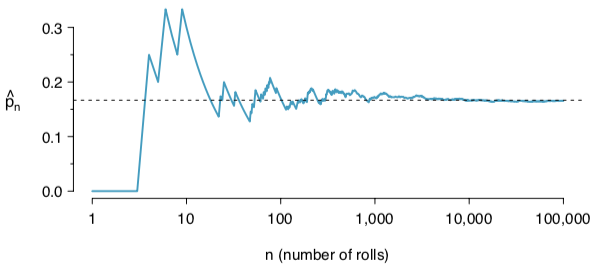
\includegraphics[scale=0.5]{images/lln.png}
    \end{center}
    With real-world data, we usually don't get a chance to see what happens when $n$ gets really big... but with simulations, we can see the Law of Large Numbers in action.
\end{frame}

\begin{frame}{Probability Notation}
    We have some shorthand notation for talking about probabilities.
    \begin{itemize}
        \item We denote "the probability of rolling a \texttt{1}" as P(rolling a \texttt{1}).
        \item As we get more comfortable with our notation, (assuming it's clear that we're talking about rolling a die) we may shorten this further to P(1).
        \item So we can write 
        \[P(\text{rolling a \texttt{1}}) = P(1) = 1/6.\]
    \end{itemize}
\end{frame}

\begin{frame}{Random Processes}
    Can you think of any other random processes we might want to examine? What are the possible outcomes?
\end{frame}

\begin{frame}{Random Processes}
    Here are a few random processes:
    \begin{itemize}
        \item Flipping a coin
        \item Wait time (in minutes) at the DMV
        \item How many hours of sleep you get each night
    \end{itemize}
    Some of these aren't completely random (the DMV is probably less crowded on, say, Tuesday mornings), but we may still want to model them based on random processes.
\end{frame}

\begin{frame}{Disjoint Outcomes}
    Two outcomes are \textbf{disjoint} or \textbf{mutually exclusive} if they cannot both happen.
    \begin{itemize}
        \item If we roll our d6 only one time, we cannot roll a \texttt{1} and a \texttt{2}. 
        \begin{itemize}
            \item On any single roll, the outcomes "rolling a \texttt{1}" and "rolling a \texttt{2}" are disjoint.
        \end{itemize}
        \item If one of a set of disjoint outcomes happens, it is impossible that any of the others can also happen.
    \end{itemize}
\end{frame}

\begin{frame}{Disjoint outcomes}
    It's easy to calculate probabilities for disjoint outcomes.
    
    \vspace{12pt}
    \begin{itemize}
        \item $P(\text{rolling a \texttt{1} \textbf{and} rolling a \texttt{2}}) = P(\text{\texttt{1} and \texttt{2}}) = 0$
        \begin{itemize}
            \item We can roll either a \texttt{1} or a \texttt{2}, but not both (on the same roll).
        \end{itemize}
        \item $P(\text{\texttt{1} \textbf{or} \texttt{2}}) = P(\text{\texttt{1}}) + P(\text{\texttt{2}}) = 1/6 + 1/6 = 1/3$
        \begin{itemize}
            \item If we want to roll a \texttt{1} or \texttt{2}, we have a 2-out-of-6 or $2/6=1/3$ chance.
        \end{itemize}
    \end{itemize}
\end{frame}

\begin{frame}{Addition Rule for Disjoint outcomes}
    We can formalize this relationship with the \textbf{addition rule for disjoint outcomes}. Suppose $A_1$ and $A_2$ are two disjoint outcomes. Then
    \[
        P(A_1 \text{ or } A_2) = P(A_1)+P(A_2).
    \]
    This can be extended to many disjoint outcomes $A_1, \dots, A_k$ where the probability that at least one of these outcomes will occur is
    \[
        P(A_1)+P(A_2)+\dots+P(A_k).
    \]
\end{frame}

\begin{frame}{Example}
    Recall our contingency table for \texttt{homeownership} and \texttt{apptype}: 
    \begin{center}
        \begin{tabular}{r l ccc r}
		& & \multicolumn{3}{c}{{\texttt{homeownership}}} & \\
        \cline{3-5}
		& & Rent & Mortgage & Own & Total  \\ 
        \cline{2-6}
        \multirow{2}{*}{{\texttt{apptype}}} 
        & Individual & 3496 & 3839 & 1170 & 8505 \\ 
  		& Joint & 362 & 950 & 183 & 1495 \\ 
        \cline{2-6}
  		& Total	& 3858 & 4789 & 1353 & 10000 \\
        \cline{2-6}
    \end{tabular}
    \end{center}
    \begin{enumerate}
        \item Are the outcomes Rent, Mortgage, and Own disjoint? Are Rent and Individual disjoint?
        \item What is the probability that someone applied for a joint loan? That someone is a renter and applied for an individual loan?
        \item Compute the probability that someone has a mortgage or owns their home.
    \end{enumerate}
\end{frame}

\begin{frame}{Example}
    \textbf{Are the outcomes Rent, Mortgage, and Own disjoint? Are Rent and Individual disjoint?}
    \begin{center}
        \begin{tabular}{r l ccc r}
		& & \multicolumn{3}{c}{{\texttt{homeownership}}} & \\
        \cline{3-5}
		& & Rent & Mortgage & Own & Total  \\ 
        \cline{2-6}
        \multirow{2}{*}{{\texttt{apptype}}} 
        & Individual & 3496 & 3839 & 1170 & 8505 \\ 
  		& Joint & 362 & 950 & 183 & 1495 \\ 
        \cline{2-6}
  		& Total	& 3858 & 4789 & 1353 & 10000 \\
        \cline{2-6}
    \end{tabular}
    \end{center}
    \vspace{12pt}Rent, Mortgage, and Own are disjoint outcomes. Someone either rents \textit{or} has a mortgage \textit{or} owns their home outright.
    
    \vspace{12pt}Rent and Individual are \textit{not} disjoint outcomes. It is possible to be a renter and apply individually for a loan.
\end{frame}

\begin{frame}{Example}
    \textbf{What is the probability that someone applied for a joint loan? That someone is a renter and applied for an individual loan?}
    \begin{center}
        \begin{tabular}{r l ccc r}
		& & \multicolumn{3}{c}{{\texttt{homeownership}}} & \\
        \cline{3-5}
		& & Rent & Mortgage & Own & Total  \\ 
        \cline{2-6}
        \multirow{2}{*}{{\texttt{apptype}}} 
        & Individual & 3496 & 3839 & 1170 & 8505 \\ 
  		& Joint & 362 & 950 & 183 & 1495 \\ 
        \cline{2-6}
  		& Total	& 3858 & 4789 & 1353 & 10000 \\
        \cline{2-6}
    \end{tabular}
    \end{center}
    \vspace{12pt}$P(\text{joint loan}) = 1495/10000 = 0.1495$ or 14.95\%.
    
    \vspace{12pt}$P(\text{rent and individual loan})=3496/10000=0.3496$ or 34.96\%.
\end{frame}

\begin{frame}{Example}
    \textbf{Compute the probability that someone has a mortgage or owns their home.}
    \begin{center}
        \begin{tabular}{r l ccc r}
		& & \multicolumn{3}{c}{{\texttt{homeownership}}} & \\
        \cline{3-5}
		& & Rent & Mortgage & Own & Total  \\ 
        \cline{2-6}
        \multirow{2}{*}{{\texttt{apptype}}} 
        & Individual & 3496 & 3839 & 1170 & 8505 \\ 
  		& Joint & 362 & 950 & 183 & 1495 \\ 
        \cline{2-6}
  		& Total	& 3858 & 4789 & 1353 & 10000 \\
        \cline{2-6}
    \end{tabular}
    \end{center}
    \vspace{12pt}We decided that these are disjoint, so we use the addition rule:
    \begin{align*}
        P(\text{mortgage or own}) &=P(\text{mortgage})+P(\text{own}) \\
        & =(4789/10000)+(1353/10000) \\
        & =6142/10000 \text{ or 61.42\%}
    \end{align*}
\end{frame}

\begin{frame}{Sets and Events}
    It is common to work with \textbf{sets} of outcomes instead of individual outcomes. We call these sets \textbf{events}.
    
    \begin{itemize}
        \item Let $A$ be the event that rolling a d6 results in a \texttt{1} or a \texttt{2}.
        \item Let $B$ be the event that rolling a d6 results in a \texttt{4} or a \texttt{6}.
        \item We write these out as $A=\{1,2\}$ and $B=\{4,6\}$.
    \end{itemize}
    Since events $A$ and $B$ have no elements (outcomes in a set) in common, they are disjoint.
\end{frame}

\begin{frame}{Sets and Events}
    Keep $A=\{1,2\}$ and $B=\{4,6\}$, and let $D$ be the event that rolling a die results in a \texttt{2} or a \texttt{3} ($D=\{2,3\}$).
    
    \vspace{12pt}Sometimes it's helpful to draw a picture when thinking about sets and probability:
    \begin{center}
        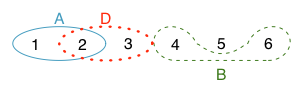
\includegraphics[scale=0.75]{images/sets.png}
    \end{center}
    Now we can see that $A$ and $B$ are disjoint; $D$ and $B$ are disjoint; but $A$ and $D$ are \textit{not} disjoint.
\end{frame}

\begin{frame}{Addition Rule for Sets?}
    The addition rule applies to sets in the same way that it applies to outcomes.
    
    \vspace{12pt}Keep $A=\{1,2\}$ and $B=\{4,6\}$. For our die, $P(A)=1/3$ and $P(B)=1/3$, so 
    \[
        P(A \text{ or } B)=P(A)+P(B)=(1/3)+(1/3)=2/3
    \]
\end{frame}

\begin{frame}{Probability for Non-Disjoint Events}
    We will use a standard 52 card deck to discuss disjoint events. If you are unfamiliar with the 52 card deck, it looks something like this:
    \begin{center}
        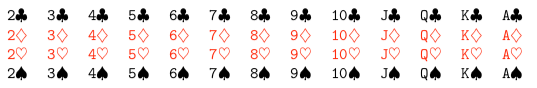
\includegraphics[scale=0.5]{images/cards.png}
    \end{center}
    \begin{itemize}
        \item 2 colors (\textcolor{red}{red} and black)
        \item 4 suits (clubs $\clubsuit$, spades $\spadesuit$, \textcolor{red}{diamonds} $\textcolor{red}{\diamondsuit}$, and \textcolor{red}{hearts} $\textcolor{red}{\heartsuit}$)
        \item In each suit, there are 13 cards labeled \texttt{2}, \texttt{3}, ..., \texttt{10}, \texttt{J} (jack), \texttt{Q} (queen), \texttt{K} (king), \texttt{A} (ace).
        \item The cards \texttt{J}, \texttt{Q}, and \texttt{K} are called the "face cards".
    \end{itemize}
\end{frame}

\begin{frame}{Venn Diagrams}
    A few slides ago, I suggested that drawing a picture might be helpful. A \textbf{Venn Diagram} is a good way to visualize the relationship between events.
    \begin{center}
        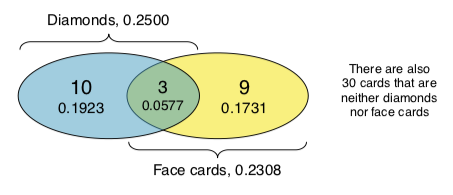
\includegraphics[scale=0.5]{images/venndiagram.png}
    \end{center}
    This Venn Diagram shows the events \texttt{Diamonds} and \texttt{Face Cards} as ovals. There are 3 face cards in the diamond suit, so the ovals overlap.
\end{frame}

\begin{frame}{Probability for Non-Disjoint Events}

    What if we want to know the probability that a randomly selected card is a \texttt{diamond} or a \texttt{face card}?

\end{frame}

\begin{frame}{Probability for Non-Disjoint Events}
    \begin{center}
        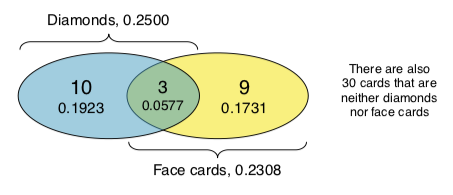
\includegraphics[scale=0.4]{images/venndiagram.png}
    \end{center}
    \begin{itemize}
        \item We start by adding up the probabilities
        \[
        P(\textcolor{red}{\diamondsuit})+P(\texttt{face card})=13/52 + 12/52
        \]
        \item But this double counts the 3 cards in the overlap!
    \end{itemize}
\end{frame}

\begin{frame}{Probability for Non-Disjoint Events}
    \begin{center}
        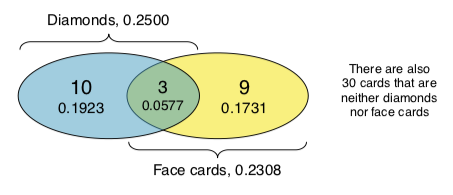
\includegraphics[scale=0.4]{images/venndiagram.png}
    \end{center}
    \begin{itemize}
        \item We need to correct for this double count:
        \begin{align*}
        P(\textcolor{red}{\diamondsuit} \text{ or } \texttt{face}) 
        & = P(\textcolor{red}{\diamondsuit})+P(\texttt{face}) - P(\textcolor{red}{\diamondsuit} \text{ and } \texttt{face}) \\
        & =13/52 + 12/52 -3/52 \\
        & = 22/52
        \end{align*}
    \end{itemize}
\end{frame}

\begin{frame}{Probability for Non-Disjoint Events}
    We can also confirm that this works by checking our deck.
    
    \begin{center}
        \includegraphics[scale=0.5]{images/cards2.png}
    \end{center}
    
    All of the cards that are a \texttt{diamond} or a \texttt{face card} are circled in purple. We can count that there are 22 of them. $22/52 = 0.42$ or 42\%.
\end{frame}

\begin{frame}{General Addition Rule}
    For any two events $A$ and $B$, the probability that at least one of them will occur is
    \[
        P(A \text{ or } B) = P(A) + P(B) - P(A \text{ and } B)
    \]
    where $P(A \text{ and } B)$ is the probability that both events occur.
    
    \vspace{18pt}Note: In statistics, whenever we say "or" we mean "and/or". If we say that "$A$ or $B$ occurs", that means $A$, $B$, or both $A$ and $B$ occur.
\end{frame}

\begin{frame}{General Addition Rule}
    By definition, for disjoint events $P(A \text{ and } B)=0$ (they can never occur simultaneously), so the general addition rule will work for both disjoint and non-disjoint events.
\end{frame}

\begin{frame}{Example}
    In the loans data set describing 10000 loans, 1495 loans were from joint applications, 4789 applicants had a mortgage, and 950 had both of these characteristics. Create a Venn diagram for this setup.
\end{frame}

\begin{frame}{Example}
    Using the Venn diagram, find the probability a randomly selected loan is from a joint application where the couple had a mortgage. What is the probability that the loan had either of these attributes (joint or mortgage)?
\end{frame}

\begin{frame}{Example}
    \textbf{Using the Venn diagram, find the probability a randomly selected loan is from a joint application where the couple had a mortgage.}
    
    \vspace{12pt}\[P(\text{joint and mortgage}) = 950/10000 = 0.095\]
\end{frame}

\begin{frame}{Example}
    \textbf{What is the probability that the loan had either of these attributes (joint or mortgage)?}
    
    \vspace{12pt}\begin{align*}
        P(\text{joint or mortgage}) &= P(\text{joint}) + P(\text{mortgage}) - P(\text{joint and mortgage}) \\
        &= (1495/10000)+(4789/10000)-(950/10000) \\
        &= 0.5334
    \end{align*}
\end{frame}

\begin{frame}{Probability Distributions}
    A \textbf{probability distribution} shows all possible (disjoint) outcomes and their corresponding probabilities.
    
    \vspace{12pt}\begin{center}
        \includegraphics[scale=0.5]{images/sum2d6.png}
    \end{center}
    This is the probability distribution for the sum of two six-sided dice.
\end{frame}

\begin{frame}{Rules for Probability Distributions}
    A probability distribution is a list of the possible outcomes with corresponding probabilities that satisfies three rules:
    \begin{enumerate}
        \item The outcomes listed must be disjoint.
        \item Each probability must be between 0 and 1.
        \item The probabilities must sum to 1.
    \end{enumerate}
    
    \vspace{12pt}We can use these rules to check whether something is a valid probability distribution.
\end{frame}

\begin{frame}{Example: Rules for Probability Distributions}
    Let's start by checking our sums for the two six-sided dice.
    \vspace{12pt}\begin{center}
        \includegraphics[scale=0.5]{images/sum2d6.png}
    \end{center}
    \begin{enumerate}
        \item The outcomes are disjoint (the two dice can't simultaneously sum to 3 \textit{and} 4).
        \item Each probability is between 0 and 1 (the minimum is 1/36 and the maximum is 6/36).
        \item The probabilities sum to 1
        \[
        \frac{1}{36}+\frac{2}{36}+\frac{3}{36}+\frac{4}{36}+\frac{5}{36}+\frac{6}{36}+\frac{5}{36}+\frac{4}{36}+\frac{3}{36}+\frac{2}{36}+\frac{1}{36}=\frac{36}{36}
        \]
    \end{enumerate}
\end{frame}

\begin{frame}{Example: Rules for Probability Distributions}
    The table below suggests 3 different distributions for household income in the US. Which one is a valid probability distribution? Why?
    
    \vspace{12pt}\begin{tabular}{r|cccc}
        \hline
        Income Range & \$0-25k & \$25k-50k & \$50k-100k & \$100k+ \\ \hline
        (a) & 0.18 & 0.39 & 0.33 & 0.16 \\
        (b) & 0.38 & -0.27 & 0.52 & 0.37 \\
        (c) & 0.28 & 0.27 & 0.29 & 0.16\\ \hline
    \end{tabular}
\end{frame}

\begin{frame}{Example: Rules for Probability Distributions}
    \begin{tabular}{r|cccc}
        \hline
        Income Range & \$0-25k & \$25k-50k & \$50k-100k & \$100k+ \\ \hline
        (a) & 0.18 & 0.39 & 0.33 & 0.16 \\
        (b) & 0.38 & -0.27 & 0.52 & 0.37 \\
        (c) & 0.28 & 0.27 & 0.29 & 0.16\\ \hline
    \end{tabular}
    
    \vspace{12pt}Let's check (a):
    \begin{enumerate}
        \item The outcomes listed must be disjoint. (TRUE)
        \item Each probability must be between 0 and 1. (TRUE)
        \item \textbf{The probabilities must sum to 1.}
        \begin{itemize}
            \item $0.18+0.39+0.33+0.16=1.16$
        \end{itemize}
    \end{enumerate}
\end{frame}

\begin{frame}{Example: Rules for Probability Distributions}
    \begin{tabular}{r|cccc}
        \hline
        Income Range & \$0-25k & \$25k-50k & \$50k-100k & \$100k+ \\ \hline
        (a) & 0.18 & 0.39 & 0.33 & 0.16 \\
        (b) & 0.38 & -0.27 & 0.52 & 0.37 \\
        (c) & 0.28 & 0.27 & 0.29 & 0.16\\ \hline
    \end{tabular}
    
    \vspace{12pt}Checking (b),
    \begin{enumerate}
        \item The outcomes listed must be disjoint. (TRUE)
        \item \textbf{Each probability must be between 0 and 1.}
        \begin{itemize}
            \item $P(\text{\$25k-50k})=-0.27$
        \end{itemize}
        \item The probabilities must sum to 1. (TRUE)
    \end{enumerate}
\end{frame}

\begin{frame}{Example: Rules for Probability Distributions}
    \begin{tabular}{r|cccc}
        \hline
        Income Range & \$0-25k & \$25k-50k & \$50k-100k & \$100k+ \\ \hline
        (a) & 0.18 & 0.39 & 0.33 & 0.16 \\
        (b) & 0.38 & -0.27 & 0.52 & 0.37 \\
        (c) & 0.28 & 0.27 & 0.29 & 0.16\\ \hline
    \end{tabular}
    
    \vspace{12pt}And checking (c),
    \begin{enumerate}
        \item The outcomes listed must be disjoint. (TRUE)
        \item Each probability must be between 0 and 1. (TRUE)
        \item The probabilities must sum to 1. (TRUE)
    \end{enumerate}
    So (c) is our valid probability distribution.
\end{frame}

\begin{frame}{Visualizing Probability Distributions}
    We can visualize this probability distribution using a bar plot.
    \begin{center}
        \includegraphics[scale=0.5]{images/probplot.png}
    \end{center}
    This is very similar to what we did when we created bar plots for proportion-based summary tables.
\end{frame}

\begin{frame}{Visualizing Probability Distributions}
    \begin{center}
        \includegraphics[scale=0.4]{images/probplot.png}
    \end{center}
    In these bar plots, the heights of the bars represent the probabilities of each event.
\end{frame}

\begin{frame}{Visualizing Probability Distributions}
    \begin{center}
        \includegraphics[scale=0.5]{images/dicesumplot.png}
    \end{center}
    This plot shows the probability distribution for the sum of the two six-sided dice.
\end{frame}

\begin{frame}{Sample Space}
    \begin{itemize}
        \item Rolling our six-sided die results in some event in the set $S=\{1,2,3,4,5,6\}$.
        \item We call this set our \textbf{sample space} ($S$). 
        \item The sample space is defined as the set of all possible outcomes.
    \end{itemize}
\end{frame}

\begin{frame}{Complement of an Event}
    Let $D=\{2,3\}$ be the event that a single roll of our d6 is a \texttt{2} or a \texttt{3}. 
    \begin{itemize}
        \item The \textbf{complement} of $D$ is the set of events in the sample space that are \textit{not} in $D$.
        \item We denote the complement by $D^c$.
        \item Then $D^c = \{1,4,5,6\}$
    \end{itemize}
    \begin{center}
        \includegraphics[scale=0.5]{images/comp.png}
    \end{center}
\end{frame}

\begin{frame}{Example: Complement of an Event}
    Let $D=\{2,3\}$ be the event that a single roll of our d6 is a \texttt{2} or a \texttt{3}. 
    
    \vspace{12pt}Find $P(D \text{ or } D^c)$. 
\end{frame}

\begin{frame}{Example: Complement of an Event}
    Let $D=\{2,3\}$ be the event that a single roll of our d6 is a \texttt{2} or a \texttt{3}. 
    
    \vspace{12pt}Find $P(D \text{ or } D^c)$. 
    \begin{itemize}
        \item First, note that an event and it's complement are always disjoint!
        \item So 
        \begin{align*}
            P(D \text{ or } D^c) &= P(D)+P(D^c) \\
            &= (1/3) + (2/3) \\
            &= 1
        \end{align*}
    \end{itemize}
\end{frame}

\begin{frame}{Example: Complement of an Event}
    Think back to possible rolls for our six-sided die. Let $A=\{1,2\}$, the event that we roll a \texttt{1} or a \texttt{2}, and $B=\{4,6\}$, the event of a \texttt{4} or a \texttt{6}.
    \begin{enumerate}
        \item What do $A^c$ and $B^c$ represent?
        \item Compute $P(A^c)$ and $P(B^c)$.
        \item Compute $P(A)+P(A^c)$ and $P(B)+P(B^c)$.
    \end{enumerate}
\end{frame}

\begin{frame}{Properties of the Complement}
    \begin{itemize}
        \item Every possible outcome not in $A$ is in $A^c$, so ($A$ or $A^c$) encompasses the entire sample space.
        \item So $P(A \text{ or } A^c)$ is the same as $P(S)$
        \item $P(S)=1$, always! 
        \begin{itemize}
            \item $S$ is all possible outcomes and there is a 100\% chance that we observe at least one of the possible outcomes.
        \end{itemize}
    \end{itemize}
\end{frame}

\begin{frame}{Properties of the Complement}
    So we can write
    \[
    P(A \text{ or } A^c) = P(A)+P(A^c)=1
    \]
    and 
    \[
    P(A) = 1-P(A^c)
    \]
    
    \vspace{12pt}Using this relationship with the complement can help us deal with more complex probability problems down the line.
\end{frame}

\begin{frame}{Example}
    \begin{center}
        \includegraphics[scale=0.5]{images/sum2d6.png}
    \end{center}
    Use the probability distribution to compute the following probabilities for rolling two six-sided dice:
    \begin{enumerate}
        \item The sum of the dice is not 6.
        \item The sum is at least 4. That is, determine the probability of the event $B = \{4, 5, ..., 12\}$.
        \item The sum is no more than 10. That is, determine the probability of the event $D = \{2, 3, ..., 10\}$.
    \end{enumerate}
\end{frame}

\begin{frame}{Example: Find $P$(sum not 6).}
    We could add all of the probabilities for the sums that are not 6... or we could use the complement!
    \begin{itemize}
        \item Let $A=\{\text{not 6}\}$ be the event that the sum is not 6.
        \item Then $A^c=\{6\}$, the event that the sum is 6.
        \item Recall 
        \begin{align*}
            P(A) &=1-P(A^c) \\
            & =1-P(6) \\
            & =1-\frac{5}{36} \\
            &= 31/36
        \end{align*}
    \end{itemize}
\end{frame}

\begin{frame}{Example: Find $P$(sum at least 4).}
    Now, we want to know if the sum is \textit{at least} 4. This means that we want to know if the sum is greater than \textit{or equal to} 4.
    \begin{itemize}
        \item Let $B=\{4,5,\dots,12\}$ be the event that the sum is at least 4.
        \item Then $B^c=\{2,3\}$, the event that the sum is less than 4.
    \end{itemize}
    \begin{align*}
            P(B) &=1-P(B^c) \\
            & =1-P(\{2,3\}) \\
            & =1-[P(3)+P(2)] \\
            & =1-\left[\frac{2}{36}+\frac{1}{36}\right] \\
            & =1-(3/36) \\
            & =11/12
        \end{align*}
\end{frame}

\begin{frame}{Example: Find $P$(sum no more than 10).}
    Now, we want to know if the sum is \textit{no more than} 10. This means that we want to know if the sum is less than \textit{or equal to} 10.
    \begin{itemize}
        \item Let $D=\{2,3,\dots,10\}$ be the event that the sum is no more than 10.
        \item Then $D^c=\{11,12\}$, the event that the sum is greater than 10.
    \end{itemize}
    \begin{align*}
            P(D) &=1-P(D^c) \\
            & =1-P(\{11,12\}) \\
            & =1-[P(11)+P(12)] \\
            & =1-\left[\frac{2}{36}+\frac{1}{36}\right] \\
            & =1-(3/36) \\
            & =11/12
        \end{align*}
\end{frame}

\begin{frame}{Midterm}
    The Midterm is next week Tuesday, August 13.
    \begin{itemize}
        \item Approximately 50 multiple choice questions.
        \item You do not need a scantron.
        \item Questions will be mostly conceptual.
        \item You may bring any basic or graphing calculator.
        \item I will bring extra scratch paper.
    \end{itemize}
\end{frame}

\begin{frame}{Extra Credit Opportunity}
    \begin{itemize}
        \item Write an exam question that would be appropriate for your midterm. 
        \item The midterm will cover material from Chapters 1, 2, and 3. 
        \item Your exam question must come from material covered in class, your homeworks, or your labs. 
        \item Questions may be either multiple choice or short answer. 
        \item To receive any credit, you must write an original question and provide both the question and the correct answer.
    \end{itemize}
    These can be submitted on iLearn (Assignments tab). It opens today at 9:30am and will close on Thursday at 11:59pm.
\end{frame}

\begin{frame}{Independence}
    \begin{itemize}
        \item Independence of random processes is similar to independence of variables and observations.
        \item We say that two random processes are \textbf{independent} if knowing the outcome of one provides no useful information about the outcome of the other.
    \end{itemize}
\end{frame}

\begin{frame}{Independence}
    For example, consider our discussion on rolling 2 six-sided dice.
    \begin{itemize}
        \item The roll of the first die has no effect on the roll of the second die.
        \item Thus our two dice rolls are independent of one another. 
    \end{itemize}
\end{frame}

\begin{frame}{Independence}
    We've already calculated the probability of the two rolls both being a \texttt{1}
    \begin{itemize}
        \item 1/6 of the time the first roll is a \texttt{1}
        \item A further 1/6 of \textit{those} times the second is also a \texttt{1}.
        \item So we decided that the probability was $(1/6)\times(1/6)=1/36$.
    \end{itemize}
    Multiplying these probabilities together works because the two events are independent.
\end{frame}

\begin{frame}{Multiplication Rule for Independent Processes}
    Let $A$ and $B$ be events from two different and independent processes. Then the probability that both $A$ and $B$ occur can be calculated as the product of their separate probabilities:
    \[ 
        P (A\text{ and }B) = P (A) \times P (B)
    \]
    Similarly, if there are $k$ events $A_1, \dots, A_k$ from $k$ independent processes, then the probability they all occur is
    \[
        P(A_1)\times P(A_2)\times\dots\times P(A_k)
    \]
\end{frame}

\begin{frame}{Example}
    About 9\% of people are left-handed. Suppose 2 people are selected at random from the U.S. population. Because the sample size of 2 is very small relative to the population, it is reasonable to assume these two people are independent.
    \begin{enumerate}
        \item What is the probability that both are left-handed?
        \item What is the probability that both are right-handed?
    \end{enumerate} 
\end{frame}

\begin{frame}{Example: Both Left-Handed}
    \textbf{What is the probability that both are left-handed?}
    \begin{itemize}
        \item Let $L_1$ be the event that the first person is left-handed and $L_2$ the event that the second person is left-handed.
        \item We are told that 9\% of people are left-handed, so $P(L_1)=P(L_2)=0.09$.
    \end{itemize}
\end{frame}

\begin{frame}{Example: Both Left-Handed}
    \textbf{What is the probability that both are left-handed?}
    \begin{itemize}
        \item We are assuming that these people are independent, so we can use the multiplication rule:
        \begin{align*}
        P(L_1\text{ and }L_2) &= P(L_1) \times P(L_2) \\
        &= (0.09)\times(0.09) \\
        &= 0.0081
        \end{align*}
        or 0.81\% (this is highly unlikely!)
    \end{itemize}
\end{frame}

\begin{frame}{Example: Both Right-Handed}
    \textbf{What is the probability that both are right-handed?}
    \begin{itemize}
        \item First, assume that everyone is either right- or left-handed.
        \item Then $L_1^c$ is the event that the first person is right-handed and $L_2^c$ is the event that the second person is right-handed.
        \item From the previous slide, we decided that $P(L_1)=P(L_2)=0.09$
        \item So $P(L_1^c)=1-P(L_1)=1-0.09=0.91$ and $P(L_2^c)=0.91$
    \end{itemize}
\end{frame}

\begin{frame}{Example: Both Right-Handed}
    \textbf{What is the probability that both are right-handed?}
    \begin{itemize}
        \item We are still assuming that these people are independent, so we can again use the multiplication rule:
        \begin{align*}
        P(L_1^c\text{ and }L_2^c) &= P(L_1^c) \times P(L_2^c) \\
        &= (0.91)\times(0.91) \\
        &= 0.8281
        \end{align*}
        or 82.81\%.
    \end{itemize}
\end{frame}

\begin{frame}{Disjoint Events - Independent?}
    If two events are disjoint, are they independent?
\end{frame}

\begin{frame}{Disjoint Events- Independent?}
    If two events are disjoint, are they independent?
    \begin{itemize}
        \item Recall that independent events have no relationship with one another.
        \item This means that if we know something about event $A$, we don't get any information about event $B$.
        \item For disjoint events, if event $A$ occurs, we can be totally certain that event $B$ did not occur.
        \item Therefore they are \textit{dependent}.
    \end{itemize}
\end{frame}

\begin{frame}{Example}
    Consider two disjoint events for rolling a six-sided die. Let $A=\{1\}$ be the event that I roll a \texttt{1} and $B=\{2\}$ the event that I roll a \texttt{2}. 
    \begin{itemize}
        \item If I know that $A$ occurred, then I can be 100\% sure that $B$ did not occur.
        \item If I know that $A$ did not occur, then I know that the roll must be a \texttt{2}, \texttt{3}, \texttt{4}, \texttt{5}, or \texttt{6}. 
        \begin{itemize}
            \item Now there are five possible options instead of six!
            \item We've narrowed down our options, so knowing that I did not roll a \texttt{1} has given us some useful information.
        \end{itemize}
    \end{itemize}
    Therefore $A$ and $B$ can't be independent.
\end{frame}
%\input{Sections/s3_1add.tex}
%\section{Section 3.2}
%\begin{frame}{Conditional Probability}
    We can get far more information out of the relationships between multiple variables than we can from a single variable.
    
    For example
    \begin{itemize}
        \item Recall our case study on the malaria vaccine.
        \item We can look at P(infection), but that doesn't tell us anything about the efficacy of the vaccine.
        \item Instead, we want to look at the probability that a person develops infection \textit{if they were vaccinated}.
        \item We compare this to the probability that a person develops infection if they were not vaccinated.
    \end{itemize}
\end{frame}

\begin{frame}{Contingency Table Probabilities}
    Let's consider a data set on a machine learning classifier. 
    \begin{itemize}
        \item The classifier is designed to take images and determine whether each one is about fashion.
        \item The classifier groups 1822 photos into either "fashion" or "not fashion".
        \item Separately, these photos are grouped into "fashion" and "not fashion" by a group of people.
        \begin{itemize}
            \item We take these groupings as the truth that the classifier is trying to get at.
        \end{itemize}
    \end{itemize}
\end{frame}

\begin{frame}{Contingency Table Probabilities}
    We can take these groupings and build them into a contingency table.
    \begin{center}
        \begin{tabular}{r l cc r}
		& & \multicolumn{2}{c}{{\texttt{truth}}} & \\
        \cline{3-4}
		& & Fashion & Not & Total  \\ 
        \cline{2-5}
        \multirow{2}{*}{{\texttt{classifier}}} 
        & Fashion   & 197 & 22 & 219 \\ 
  		& Not       & 112 & 1491 & 1603 \\ 
        \cline{2-5}
  		& Total	& 309 & 1513 & 1822 \\
        \cline{2-5}
    \end{tabular}
    \end{center}
\end{frame}

\begin{frame}{Contingency Table Probabilities}
    We think about this a lot with classification problems! 
    \begin{center}
        \begin{tabular}{r l cc r}
		& & \multicolumn{2}{c}{{\texttt{truth}}} & \\
        \cline{3-4}
		& & \texttt{fashion} & \texttt{not fashion} & Total  \\ 
        \cline{2-5}
        \multirow{2}{*}{{\texttt{classifier}}} 
        & \texttt{pred fashion}   & 197 & 22 & 219 \\ 
  		& \texttt{pred not}       & 112 & 1491 & 1603 \\ 
        \cline{2-5}
  		& Total	& 309 & 1513 & 1822 \\
        \cline{2-5}
    \end{tabular}
    \end{center}
    \begin{itemize}
        \item When we build our classifier, we want to know the rate at which it correctly and incorrectly identifies \texttt{fashion} and \texttt{not fashion}.
        \item This will give us an idea of how successful our classifier is.
        \begin{itemize}
            \item Is it a good classifier?
            \item Should we try a different machine learning algorithm?
        \end{itemize}
    \end{itemize}
\end{frame}

\begin{frame}{Example: Contingency Table Probabilities}
    \begin{enumerate}
        \item If the photo is actually about fashion, what is the probability that the classifier correctly identified it as being about fashion?
        \item If the classifier predicted that a photo was not about fashion, what is the probability that it was incorrect?
    \end{enumerate}
\end{frame}

\begin{frame}{Example: Contingency Table Probabilities}
    \textbf{If the photo is actually about fashion, what is the probability that the classifier correctly identified it as being about fashion?}
    \begin{center}
        \begin{tabular}{r l cc r}
		& & \multicolumn{2}{c}{{\texttt{truth}}} & \\
        \cline{3-4}
		& & \texttt{fashion} & \texttt{not fashion} & Total  \\ 
        \cline{2-5}
        \multirow{2}{*}{{\texttt{classifier}}} 
        & \texttt{pred fashion}   & 197 & 22 & 219 \\ 
  		& \texttt{pred not}       & 112 & 1491 & 1603 \\ 
        \cline{2-5}
  		& Total	& 309 & 1513 & 1822 \\
        \cline{2-5}
    \end{tabular}
    \end{center}
    \begin{itemize}
        \item We know that the photo is actually about fashion, so we focus our attention to the column where \texttt{truth} is \texttt{fashion}. 
        \item Then within this column, we look for the number of times the classifier \texttt{pred fashion} out of the total number of \texttt{fashion} photos.
    \end{itemize}
\end{frame}

\begin{frame}{Example: Contingency Table Probabilities}
    \textbf{If the photo is actually about fashion, what is the probability that the classifier correctly identified it as being about fashion?}
    \begin{center}
        \begin{tabular}{r l cc r}
		& & \multicolumn{2}{c}{{\texttt{truth}}} & \\
        \cline{3-4}
		& & \texttt{fashion} & \texttt{not fashion} & Total  \\ 
        \cline{2-5}
        \multirow{2}{*}{{\texttt{classifier}}} 
        & \texttt{pred fashion}   & 197 & 22 & 219 \\ 
  		& \texttt{pred not}       & 112 & 1491 & 1603 \\ 
        \cline{2-5}
  		& Total	& 309 & 1513 & 1822 \\
        \cline{2-5}
    \end{tabular}
    \end{center}
    \[
    P(\texttt{classifier}\text{ is }\texttt{pred fashion}\textit{ given }\texttt{truth}\text{ is }\texttt{fashion}) = \frac{197}{309}
    \]
    or 0.638, a reasonable correct identification rate for fashion.
\end{frame}

\begin{frame}{Example: Contingency Table Probabilities}
    \textbf{If the classifier predicted that a photo was not about fashion, what is the probability that it was incorrect?}
    \begin{center}
        \begin{tabular}{r l cc r}
		& & \multicolumn{2}{c}{{\texttt{truth}}} & \\
        \cline{3-4}
		& & \texttt{fashion} & \texttt{not fashion} & Total  \\ 
        \cline{2-5}
        \multirow{2}{*}{{\texttt{classifier}}} 
        & \texttt{pred fashion}   & 197 & 22 & 219 \\ 
  		& \texttt{pred not}       & 112 & 1491 & 1603 \\ 
        \cline{2-5}
  		& Total	& 309 & 1513 & 1822 \\
        \cline{2-5}
    \end{tabular}
    \end{center}
    \begin{itemize}
        \item We know that \texttt{classifier} is \texttt{pred not} fashion, so we focus our attention to this row.
        \item We want to know the probability that it was incorrect, or in \texttt{truth} is \texttt{fashion}.
    \end{itemize}
\end{frame}

\begin{frame}{Example: Contingency Table Probabilities}
    \textbf{If the classifier predicted that a photo was not about fashion, what is the probability that it was incorrect?}
    \begin{center}
        \begin{tabular}{r l cc r}
		& & \multicolumn{2}{c}{{\texttt{truth}}} & \\
        \cline{3-4}
		& & \texttt{fashion} & \texttt{not fashion} & Total  \\ 
        \cline{2-5}
        \multirow{2}{*}{{\texttt{classifier}}} 
        & \texttt{pred fashion}   & 197 & 22 & 219 \\ 
  		& \texttt{pred not}       & 112 & 1491 & 1603 \\ 
        \cline{2-5}
  		& Total	& 309 & 1513 & 1822 \\
        \cline{2-5}
    \end{tabular}
    \end{center}
    \[
    P(\texttt{truth}\text{ is }\texttt{fashion}\textit{ given }\texttt{classifier}\text{ is }\texttt{pred not}) = \frac{112}{1603}
    \]
    or 0.070, a low misidentification rate for fashion photos. 
\end{frame}

\begin{frame}{Marginal and Joint Probabilities}
    \begin{center}
        \begin{tabular}{r l cc r}
		& & \multicolumn{2}{c}{{\texttt{truth}}} & \\
        \cline{3-4}
		& & \texttt{fashion} & \texttt{not fashion} & Total  \\ 
        \cline{2-5}
        \multirow{2}{*}{{\texttt{classifier}}} 
        & \texttt{pred fashion}   & 197 & 22 & 219 \\ 
  		& \texttt{pred not}       & 112 & 1491 & 1603 \\ 
        \cline{2-5}
  		& Total	& 309 & 1513 & 1822 \\
        \cline{2-5}
    \end{tabular}
    \end{center}
    \begin{itemize}
        \item We've now used our contingency table to think about two types of probabilities.
        \begin{itemize}
            \item The probability for a single event (from the row and column of totals).
            \item The probability for multiple events together (from the numbers in the middle).
        \end{itemize}
    \end{itemize}
\end{frame}

\begin{frame}{Marginal Probabilities}
    \begin{itemize}
        \item A \textbf{marginal probability} is a probability based on a single variable.
        \item Think of the \textit{margins} as the edges of a contingency table where we have the information for each variable individually.
    \end{itemize}
\end{frame}

\begin{frame}{Marginal Probabilities}
    \begin{center}
        \begin{tabular}{r l cc r}
		& & \multicolumn{2}{c}{{\texttt{truth}}} & \\
        \cline{3-4}
		& & \texttt{fashion} & \texttt{not fashion} & Total  \\ 
        \cline{2-5}
        \multirow{2}{*}{{\texttt{classifier}}} 
        & \texttt{pred fashion}   & 197 & 22 & 219 \\ 
  		& \texttt{pred not}       & 112 & 1491 & 1603 \\ 
        \cline{2-5}
  		& Total	& 309 & 1513 & 1822 \\
        \cline{2-5}
    \end{tabular}
    \end{center}
    \vspace{10pt}A probability based solely on our \texttt{classifier} is a marginal probability. It is based on a single variable without regard to any other variables. 
    \[
    P(\texttt{classifier} \text{ is } \texttt{pred fashion}) = 219/1822
    \]
\end{frame}

\begin{frame}{Joint Probabilities}
    \begin{itemize}
        \item A \textbf{joint probability} is a probability for two or more variables together.
        \item Think of this as a probability that two or more variables occur \textit{jointly} (together). 
    \end{itemize}
\end{frame}

\begin{frame}{Joint Probabilities}
    \begin{center}
        \begin{tabular}{r l cc r}
		& & \multicolumn{2}{c}{{\texttt{truth}}} & \\
        \cline{3-4}
		& & \texttt{fashion} & \texttt{not fashion} & Total  \\ 
        \cline{2-5}
        \multirow{2}{*}{{\texttt{classifier}}} 
        & \texttt{pred fashion}   & 197 & 22 & 219 \\ 
  		& \texttt{pred not}       & 112 & 1491 & 1603 \\ 
        \cline{2-5}
  		& Total	& 309 & 1513 & 1822 \\
        \cline{2-5}
    \end{tabular}
    \end{center}
    \vspace{10pt}The probability that our \texttt{classifier} is \texttt{pred fashion} and the truth is \texttt{fashion} is a joint probability. It is based on two variables together. 
    \[
    P(\texttt{classifier} \text{ is } \texttt{pred fashion} \text { and } \texttt{truth} \text{ is } \texttt{fashion}) = 197/1822
    \]
\end{frame}

\begin{frame}{Table Proportions}
    We can examine marginal and joint probabilities using table proportions. \textbf{Table proportions} are computed by dividing each count in a contingency table by the table's grand total.
    \begin{center}
        \begin{tabular}{r l cc r}
		& & \multicolumn{2}{c}{{\texttt{truth}}} & \\
        \cline{3-4}
		& & \texttt{fashion} & \texttt{not fashion} & Total  \\ 
        \cline{2-5}
        \multirow{2}{*}{{\texttt{classifier}}} 
        & \texttt{pred fashion}   & 0.108 & 0.012 & 0.120 \\ 
  		& \texttt{pred not}       & 0.062 & 0.818 & 0.880 \\ 
        \cline{2-5}
  		& Total	& 0.170 & 0.830 & 1.000 \\
        \cline{2-5}
    \end{tabular}
    \end{center}
\end{frame}

\begin{frame}{Joint Probability Distributions}
    A joint probability distribution is just a probability distribution for multiple variables together.
    \begin{center}
        \small
        \begin{tabular}{l c}
            Joint Outcome & Probability \\ 
            \hline
            \texttt{classifier} is \texttt{pred fashion} and \texttt{truth} is \texttt{fashion} & 0.108 \\
            \texttt{classifier} is \texttt{pred fashion} and \texttt{truth} is \texttt{not fashion} & 0.012 \\
            \texttt{classifier} is \texttt{pred not} and \texttt{truth} is \texttt{fashion} & 0.062 \\
            \texttt{classifier} is \texttt{pred not} and \texttt{truth} is \texttt{not fashion} & 0.818 \\
            \hline
            Total & 1.000 \\
            \hline 
        \end{tabular}
    \end{center}

    Note: A marginal probability distribution is the type of probability distribution we introduced last week!
\end{frame}

\begin{frame}{Marginal and Joint Probabilities}
    We can compute marginal probabilities using joint probabilities. 
    \begin{center}
        \small
        \begin{tabular}{l c}
            Joint Outcome & Probability \\ 
            \hline
            \texttt{classifier} is \texttt{pred fashion} and \texttt{truth} is \texttt{fashion} & 0.108 \\
            \texttt{classifier} is \texttt{pred fashion} and \texttt{truth} is \texttt{not fashion} & 0.012 \\
            \texttt{classifier} is \texttt{pred not} and \texttt{truth} is \texttt{fashion} & 0.062 \\
            \texttt{classifier} is \texttt{pred not} and \texttt{truth} is \texttt{not fashion} & 0.818 \\
            \hline
            Total & 1.000 \\
            \hline 
        \end{tabular}
    \end{center}
    For example, 
    \begin{align*}
    P(\texttt{truth}& \text{ is } \texttt{fashion}) \\ 
    =& P(\texttt{classifier} \text{ is } \texttt{pred fashion} \text{ and } \texttt{truth} \text{ is } \texttt{fashion}) \\
    &+ P(\texttt{classifier} \text{ is } \texttt{pred not} \text{ and } \texttt{truth} \text{ is } \texttt{fashion}) \\
    =& 0.108 + 0.062 \\
    =& 0.170
    \end{align*}
\end{frame}

\begin{frame}{Marginal and Joint Probabilities}
    This makes sense based on our table proportions!
    \begin{center}
        \begin{tabular}{r l cc r}
		& & \multicolumn{2}{c}{{\texttt{truth}}} & \\
        \cline{3-4}
		& & \texttt{fashion} & \texttt{not fashion} & Total  \\ 
        \cline{2-5}
        \multirow{2}{*}{{\texttt{classifier}}} 
        & \texttt{pred fashion}   & 0.108 & 0.012 & 0.120 \\ 
  		& \texttt{pred not}       & 0.062 & 0.818 & 0.880 \\ 
        \cline{2-5}
  		& Total	& 0.170 & 0.830 & 1.000 \\
        \cline{2-5}
    \end{tabular}
    \end{center}
    \begin{itemize}
        \item All of these numbers are directly proportional to our original contingency table.
        \item The row and column of totals represent the marginal probabilities.
        \item These totals are the actual sums of their respective rows/columns.
    \end{itemize}
\end{frame}

\begin{frame}{Defining Conditional Probability}
    \begin{itemize}
        \item The \texttt{classifier} predicts whether a photo is about \texttt{fashion}, but it is not perfect.
        \item We'd like to know how we can use these predictions to improve our understanding of the second variable, the \texttt{truth}.
        \item We might want to know, for example, the probability that the \texttt{truth} is \texttt{fashion} \textit{given} that the \texttt{classifier predicts fashion}. 
    \end{itemize}
\end{frame}

\begin{frame}{Defining Conditional Probability}
    The probability that a random photo from the data set is actually about fashion is 0.17. Suppose we know that \texttt{classifier} is \texttt{pred fashion}.
    \begin{itemize}
        \item Now we can get a better estimate of the probability that the \texttt{truth} is \texttt{fashion}.
        \item We do this by restricting our attention to the 219 cases where the \texttt{classifier} is \texttt{pred fashion}.
        \item Then we look at the fraction of \textit{these} photos where the \texttt{truth} is \texttt{fashion} (197 cases).
    \end{itemize}
    \[
    P(\texttt{truth} \text{ is } \texttt{fashion} \text{ given } \texttt{classifier} \text{ is } \texttt{pred fashion}) = \frac{197}{219}
    \]
\end{frame}

\begin{frame}{Defining Conditional Probability}
    \begin{itemize}
        \item When we are given some useful information that allows us to restrict our attention, we call these probabilities \textbf{conditional probabilities}. 
        \item We can say that we condition based on some \textit{given} information, or that we computed the probability under the \textit{condition} that the \texttt{classifier} is \texttt{pred fashion}.
    \end{itemize}
\end{frame}

\begin{frame}{Defining Conditional Probability}
    There are two important aspects to a conditional probability:
    \begin{enumerate}
        \item The \textbf{outcome of interest} is whatever we want to know about.
        \item The \textbf{condition} is information we know to be true, a known outcome or event.
    \end{enumerate}
\end{frame}

\begin{frame}{Conditional Probability Notation}
    We separate our outcome of interest from our condition in our probability notation with a vertical bar:
    \[
    P(\texttt{truth} \text{ is } \texttt{fashion} \text{ given } \texttt{classifier} \text{ is } \texttt{pred fashion})
    \]
    becomes
    \[
    P(\texttt{truth} \text{ is } \texttt{fashion } | \texttt{ classifier} \text{ is } \texttt{pred fashion}) = \frac{197}{219}
    \]
    We read the vertical bar as the word \textit{given}.
\end{frame}

\begin{frame}{Defining Conditional Probability}
    Earlier, we computed 
    \[
    P(\texttt{truth} \text{ is } \texttt{fashion} \text{ given } \texttt{classifier} \text{ is } \texttt{pred fashion}) = 0.900
    \]
    by restricting our attention to the data where \texttt{classifier} is \texttt{pred fashion}. 
    
    \vspace{12pt}From this row where \texttt{classifier} is \texttt{pred fashion}, we took the number of cases where \texttt{truth} is \texttt{fashion} and divided by the row total to get our answer. 
\end{frame}

\begin{frame}{Defining Conditional Probability}
    However, we don't always have access to the count data. Instead we are given only the probabilities. 
    \begin{center}
        \begin{tabular}{r l cc r}
		& & \multicolumn{2}{c}{{\texttt{truth}}} & \\
        \cline{3-4}
		& & \texttt{fashion} & \texttt{not fashion} & Total  \\ 
        \cline{2-5}
        \multirow{2}{*}{{\texttt{classifier}}} 
        & \texttt{pred fashion}   & 0.108 & 0.012 & 0.120 \\ 
  		& \texttt{pred not}       & 0.062 & 0.818 & 0.880 \\ 
        \cline{2-5}
  		& Total	& 0.170 & 0.830 & 1.000 \\
        \cline{2-5}
    \end{tabular}
    \end{center}
\end{frame}

\begin{frame}{Defining Conditional Probability}    
    \begin{itemize}
        \item Suppose we took a sample of 1000 photos. 
        \item We could multiply each probability by 1000 to get an estimate of how many would fall into each place in our contingency table.
        \item We would anticipate $0.120\times1000=120$ to be the number of cases where \texttt{classifier} is \texttt{pred fashion}.
        \item We would expect to see $0.108\times1000=108$ cases where \texttt{truth} is \texttt{fashion} and \texttt{classifier} is \texttt{pred fashion}
    \end{itemize}
\end{frame}

\begin{frame}{Defining Conditional Probability} 
    We can use these numbers to compute our conditional probability. (Using our count data, we found $197/219=0.90$.)
    \begin{align*}
    P&(\texttt{truth} \text{ is } \texttt{fashion} \text{ given } \texttt{classifier} \text{ is } \texttt{pred fashion}) \\
    &= \frac{\# \text{ cases }(\texttt{truth} \text{ is } \texttt{fashion} \text{ and } \texttt{classifier} \text{ is } \texttt{pred fashion})}{\# \text{ cases (\texttt{classifier} \text{ is } \texttt{pred fashion})}} \\
    &= \frac{108}{120} = \frac{0.108\times1000}{0.120\times1000} = \frac{0.108}{0.120} = 0.90
    \end{align*}
\end{frame}

\begin{frame}{Defining Conditional Probability}
    This is the ratio, or fraction, or two probabilities. We can rewrite this as
    \begin{align*}
    P&(\texttt{truth} \text{ is } \texttt{fashion} \text{ given } \texttt{classifier} \text{ is } \texttt{pred fashion}) \\
    &= \frac{P(\texttt{truth} \text{ is } \texttt{fashion} \text{ and } \texttt{classifier} \text{ is } \texttt{pred fashion})}{P(\texttt{classifier} \text{ is } \texttt{pred fashion})} \\
    &= \frac{0.108}{0.120} = 0.90
    \end{align*}
\end{frame}

\begin{frame}{Defining Conditional Probability}
    This leads us to the general \textbf{conditional probability formula}:
    
    \vspace{12pt}Let $A$ and $B$ be outcomes. The conditional probability of outcome $A$ occurring given the condition that $B$ has occurred is
    \[
    P(A|B)=\frac{P(A\text{ and }B)}{P(B)}
    \]
\end{frame}

\begin{frame}{Example}
    Find the probability that the classifier is incorrect when classifying a photo about fashion.
\end{frame}

\begin{frame}{Example}
    \textbf{Find the probability that the classifier is incorrect when classifying a photo about fashion.}
    \begin{itemize}
        \item We \textit{know} that the photo is about fashion.
        \begin{itemize}
            \item We can write that \texttt{truth} is \texttt{fashion}.
            \item This information is given, or our condition.
        \end{itemize}
        \item From that, we want to know the probability that the classifier is wrong.
        \begin{itemize}
            \item We want to know the probability that the \texttt{classifier} results in \texttt{not fashion}.
        \end{itemize}
    \end{itemize}
\end{frame}

\begin{frame}{Example}
    \textbf{Find the probability that the classifier is incorrect when classifying a photo about fashion.}
    
    \vspace{12pt}Putting this all together, we want
        \[
        P(\texttt{classifier} \text{ is } \texttt{not fashion } | \texttt{ truth} \text{ is } \texttt{fashion})
        \]
\end{frame}

\begin{frame}{Example}
    Using our formula
    \[
    P(A|B)=\frac{P(A \text{ and }B)}{P(B)}
    \]
    we let $A$ be the event that \texttt{classifier} is \texttt{not fashion} and $B$ the event that \texttt{truth} is \texttt{fashion}. Then
    \begin{align*}
    P&(\texttt{classifier} \text{ is } \texttt{not fashion } | \texttt{ truth} \text{ is } \texttt{fashion}) \\
    &= \frac{P(\texttt{classifier} \text{ is } \texttt{not fashion } \text{and} \texttt{ truth} \text{ is } \texttt{fashion})}{P(\texttt{truth} \text{ is } \texttt{fashion})}
    \end{align*}
\end{frame}

\begin{frame}{Example}
    \begin{center}
        \begin{tabular}{r l cc r}
		& & \multicolumn{2}{c}{{\texttt{truth}}} & \\
        \cline{3-4}
		& & \texttt{fashion} & \texttt{not fashion} & Total  \\ 
        \cline{2-5}
        \multirow{2}{*}{{\texttt{classifier}}} 
        & \texttt{pred fashion}   & 0.108 & 0.012 & 0.120 \\ 
  		& \texttt{pred not}       & 0.062 & 0.818 & 0.880 \\ 
        \cline{2-5}
  		& Total	& 0.170 & 0.830 & 1.000 \\
        \cline{2-5}
    \end{tabular}
    \end{center}
    \begin{align*}
    P&(\texttt{classifier} \text{ is } \texttt{not fashion } | \texttt{ truth} \text{ is } \texttt{fashion}) \\
    &= \frac{P(\texttt{classifier} \text{ is } \texttt{not fashion } \text{and} \texttt{ truth} \text{ is } \texttt{fashion})}{P(\texttt{truth} \text{ is } \texttt{fashion})} \\
    &= \frac{0.062}{0.170} = 0.363
    \end{align*}
\end{frame}

\begin{frame}{Example: Smallpox}
    The \texttt{smallpox} data set is a sample of 6224 individuals from the year 1721. 
    \begin{center}
        \begin{tabular}{r l cc r}
		& & \multicolumn{2}{c}{{\texttt{inoculated}}} & \\
        \cline{3-4}
		& & \texttt{yes} & \texttt{no} & Total  \\ 
        \cline{2-5}
        \multirow{2}{*}{{\texttt{result}}} 
        & \texttt{lived}    & 238 & 5136 & 5374 \\ 
  		& \texttt{died}     & 6 & 844 & 850 \\ 
        \cline{2-5}
  		& Total	            & 244 & 5980 & 6224 \\
        \cline{2-5}
    \end{tabular}
    \end{center}
\end{frame}

\begin{frame}{Example: Smallpox}
    The \texttt{smallpox} data set has the following table proportions: 
    \begin{center}
        \begin{tabular}{r l cc r}
		& & \multicolumn{2}{c}{{\texttt{inoculated}}} & \\
        \cline{3-4}
		& & \texttt{yes} & \texttt{no} & Total  \\ 
        \cline{2-5}
        \multirow{2}{*}{{\texttt{result}}} 
        & \texttt{lived}    & 0.038 & 0.825 & 0.863 \\ 
  		& \texttt{died}     & 0.001 & 0.136 & 0.137 \\ 
        \cline{2-5}
  		& Total	            & 0.039 & 0.961 & 1.000 \\
        \cline{2-5}
    \end{tabular}
    \end{center}
    Let's find the probability that an inoculated person died from smallpox.
\end{frame}

\begin{frame}{Example: Smallpox}
    \textbf{Find the probability that an inoculated person died from smallpox.}
    
    \begin{itemize}
        \item We are told that the person is inoculated. This is our condition.
        \item We want to know the probability that this person died. 
        \item This is the probability that a person died given that they were inoculated
        \[
        P(\texttt{died }|\texttt{ inoculated})
        \]
    \end{itemize}
\end{frame}

\begin{frame}{Example: Smallpox}
    \textbf{Find the probability that an inoculated person died from smallpox.}
    \begin{center}
        \begin{tabular}{r l cc r}
		& & \multicolumn{2}{c}{{\texttt{inoculated}}} & \\
        \cline{3-4}
		& & \texttt{yes} & \texttt{no} & Total  \\ 
        \cline{2-5}
        \multirow{2}{*}{{\texttt{result}}} 
        & \texttt{lived}    & 0.038 & 0.825 & 0.863 \\ 
  		& \texttt{died}     & 0.001 & 0.136 & 0.137 \\ 
        \cline{2-5}
  		& Total	            & 0.039 & 0.961 & 1.000 \\
        \cline{2-5}
    \end{tabular}
    \end{center}
    \begin{align*}
        P(\texttt{died }|\texttt{ inoculated}) &= \frac{P(\texttt{died} \text{ and } \texttt{inoculated})} {P(\texttt{inoculated})} \\
        &= \frac{0.001}{0.039} = 0.026
    \end{align*}
\end{frame}

\begin{frame}{General Multiplication Rule}
    In the previous section, we talked about the multiplication rule for independent events. The \textbf{general multiplication rule} is for all events, whether or not they are independent.
    
    \vspace{12pt}Let $A$ and $B$ be any two outcomes or events. Then
    \[
    P(A \text{ and } B) = P(A|B)\times P(B)
    \]
    
    \vspace{12pt}Notice that this is not new information! This is just a rearrangement of the formula for conditional probability. 
\end{frame}

\begin{frame}{Example}
    Let's return to the \texttt{smallpox} data set, but suppose we only have two pieces of information:
    \begin{enumerate}
        \item 96.08\% of people were not inoculated.
        \item 85.88\% of people who were not inoculated ended up surviving.
    \end{enumerate}
    
    \vspace{12pt}Can we compute the probability that a resident was not inoculated and lived?
\end{frame}

\begin{frame}{Example}
    \textbf{Compute the probability that a resident was not inoculated and lived.}
    
    \vspace{12pt}First, let's rewrite the information we were given in probability notation.
    \begin{itemize}
        \item 96.08\% of people were not inoculated $\rightarrow P(\texttt{inoculated}=\texttt{no})=0.9608$
        \item 85.88\% of people who were not inoculated ended up surviving $\rightarrow P(\texttt{result}=\texttt{lived }|\texttt{ inoculated}=\texttt{no})=0.8588$
    \end{itemize}
\end{frame}

\begin{frame}{Example}
    \textbf{Compute the probability that a resident was not inoculated and lived.}
    
    \vspace{12pt}Then we use this information with the general multiplication rule.
    \begin{align*}
        P&(\texttt{result}=\texttt{lived} \text{ and } \texttt{inoculated}=\texttt{no}) \\
        &=P(\texttt{result}=\texttt{lived } | \texttt{ inoculated}=\texttt{no})\times P(\texttt{inoculated}=\texttt{no}) \\
        &= 0.9608\times08588 \\
        &= 0.8251.
    \end{align*}
\end{frame}

\begin{frame}{Sum of Conditional Probabilities}
    Let $A_1, \dots, A_k$ represent all the disjoint outcomes for a variable or process. Then if $B$ is some event,
    \[
        P(A_1|B) + \dots + P(A_k|B) = 1
    \]
    The rule for complements also holds when an event and its complement are conditioned on the same information:
    \[
    P(A|B) = 1 − P(A^c|B)
    \]
    Why are these true? Let's look at a Venn diagram.
\end{frame}

\begin{frame}{Independence Considerations}
    For two independent events, knowing the outcome of one should give us no information about the probability of the other. Consider $X$ and $Y$, the outcomes for rolling two six-sided dice.
    \begin{enumerate}
        \item Find $P(X=1)$.
        \item Find $P(X=1 \text{ and }Y=1)$.
        \item Find $P(Y=1|X=1)$.
    \end{enumerate}
    Knowing the outcome of $X$ doesn't give us any additional information about $Y$.
\end{frame}

\begin{frame}{Independence Considerations}
    We can use the Multiplication Rule to show that the conditioning information has no influence for independent processes:
    \begin{align*}
        P(Y=1|X=1) &= \frac{P(Y=1\text{ and }X=1)}{P(X=1)} \\
        &= \frac{P(Y=1)P(X=1)}{P(X=1)} \\
        &= P(Y=1)
    \end{align*}
\end{frame}

\begin{frame}{Example: The Gambler's Fallacy}
    A roulette wheel has 18 black slots, 18 red slots, and 2 green slots (38 total slots). 

    \vspace{12pt}Ron is watching a roulette table in a casino and notices that the last five outcomes were \texttt{black}. He figures that the chances of getting \texttt{black} six times in a row is very small (about 1/64) and puts his paycheck on \texttt{red}. 
    
    \vspace{12pt}What is wrong with his reasoning?
\end{frame}

\begin{frame}{Example: The Gambler's Fallacy}
    What is wrong with Ron's reasoning?
    \begin{itemize}
        \item It's true that there is close to a $1/64=0.016$ chance that we get \texttt{black} six times in a row.
        \begin{itemize}
            \item $P(\texttt{black}_1)\times\dots\times P(\texttt{black}_5)\times P(\texttt{black}_6) = (9/19)^6 = 0.011$
        \end{itemize}
        \item But there's also a 1/64 chance that we get \texttt{black} five times in a row followed by \texttt{red}.
        \begin{itemize}
            \item $P(\texttt{black}_1)\times\dots\times P(\texttt{black}_5)\times P(\texttt{red}_6) = (9/19)^6 = 0.011$
        \end{itemize}
    \end{itemize}
\end{frame}

\begin{frame}{Example: The Gambler's Fallacy}
    What is wrong with Ron's reasoning?
    \begin{itemize}
        \item Each spin is independent of the previous spins!
        \item This means that each spin has a 18/38 chance of being \texttt{black}!
        \item Ron has a $1-\frac{18}{38}=0.538$ chance of losing his entire paycheck. 
    \end{itemize}
\end{frame}

\begin{frame}{Tree Diagrams}
    \textbf{Tree diagrams} help organize outcomes and probabilities based on the structure of the data. They are especially useful when the data can be put into some kind of sequential structure.
\end{frame}

\begin{frame}{Tree Diagrams}
    \begin{itemize}
        \item The \texttt{smallpox} data can be structured this way. 
        \item We split the data by \texttt{inoculation} (\texttt{yes} or \texttt{no}).
        \item Then we split by \texttt{result} (\texttt{lived} or \texttt{died}).
    \end{itemize}
\end{frame}

\begin{frame}{Tree Diagrams}
    \begin{center}
        \includegraphics[scale=0.5]{images/tree.png}
    \end{center}
\end{frame}

\begin{frame}{Tree Diagrams}
    \begin{center}
        \includegraphics[scale=0.3]{images/tree.png}
    \end{center}
    \begin{itemize}
        \item The first branch, for \texttt{inoculation}, is called the \textbf{primary branch}.
        \item All other branches, in this case for \texttt{result} are \textbf{secondary branches}.
    \end{itemize}
\end{frame}

\begin{frame}{Tree Diagrams}
    \begin{center}
        \includegraphics[scale=0.3]{images/tree.png}
    \end{center}
    \begin{itemize}
        \item The probabilities for the primary branch are marginal.
        \begin{itemize}
            \item For \texttt{inoculation} is \texttt{yes}, the marginal probability is $P(\texttt{inoculation} \text{ is } \texttt{yes})=0.0392$.
        \end{itemize}
        \item The probabilities for the secondary branches are conditional.
        \begin{itemize}
            \item For \texttt{result} is \texttt{lived} on the \texttt{inoculation} is \texttt{yes} branch, we have $P(\texttt{result} \text{ is } \texttt{lived } |\texttt{ inoculation} \text{ is } \texttt{yes})=0.9754$
        \end{itemize}
    \end{itemize}
\end{frame}

\begin{frame}{Tree Diagrams}
    \begin{center}
        \includegraphics[scale=0.3]{images/tree.png}
    \end{center}
    \begin{itemize}
        \item Joint probabilities are shown to the right of each secondary branch.
        \item These are computed using the General Multiplication Rule
        \[
        P(A\text{ and }B)=P(A|B)\times P(B)
        \]
        where the primary branch represents event $B$ and the secondary branch event $A$.
    \end{itemize}
\end{frame}

\begin{frame}{Example: Exam Scores}
    Consider the midterm and final for a statistics class. 
    \begin{itemize}
        \item Suppose 13\% of students earned an A on the midterm. 
        \item Of those students who earned an A on the midterm, 47\% received an A on the final.
        \item 11\% of the students who earned lower than an A on the midterm received an A on the final.
        \item You pick up a final exam at random and notice the student received an A.
    \end{itemize} 
    What is the probability that this student earned an A on the midterm?
\end{frame}

\begin{frame}{Example: Exam Scores}
    Let's start by writing the given information in probability notation.
    \begin{itemize}
        \item $P(\texttt{midterm}=\texttt{A})=0.13$
        \item $P(\texttt{final}=\texttt{A } | \texttt{ midterm}=\texttt{A})=0.47$
        \item $P(\texttt{final}=\texttt{A } | \texttt{ midterm}=\texttt{not A})=0.11$
    \end{itemize}
    \vspace{12pt}We want to know the probability that a student who earned an A on the final also earned an A on the midterm:
    \[
    P(\texttt{midterm}=\texttt{A }|\texttt{ final}=\texttt{A})
    \]
\end{frame}

\begin{frame}{Example: Exam Scores}
    Now that we've formalized the information from the problem statement, we can consider our next steps.
    
    \vspace{12pt}It's not yet clear how to calculate 
    \[P(\texttt{midterm}=\texttt{A }|\texttt{ final}=\texttt{A}),\]
    so let's use what we know to draw a tree diagram.
\end{frame}

\begin{frame}{Example: Exam Scores}
    We will use this information to draw our tree diagram.
    \begin{itemize}
        \item $P(\texttt{midterm}=\texttt{A})=0.13$
        \item $P(\texttt{final}=\texttt{A } | \texttt{ midterm}=\texttt{A})=0.47$
        \item $P(\texttt{final}=\texttt{A } | \texttt{ midterm}=\texttt{not A})=0.11$
    \end{itemize}
\end{frame}

\begin{frame}{Example: Exam Scores}
    \begin{center}
        \includegraphics[scale=0.5]{images/tree2.png}
    \end{center}
    Can we use this to calculate $P(\texttt{midterm}=\texttt{A }|\texttt{ final}=\texttt{A})$?
\end{frame}

\begin{frame}{Example: Exam Scores}
    First, consider our conditional probability formula.
    \[
        P(\texttt{midterm}=\texttt{A }|\texttt{ final}=\texttt{A}) = \frac{P(\texttt{midterm}=\texttt{A }\text{and}\texttt{ final}=\texttt{A})}{P(\texttt{final}=\texttt{A})}
    \]
    We can get all of the probabilities on the right hand side of the formula by using our tree diagram!
\end{frame}

\begin{frame}{Example: Exam Scores}
    \begin{center}
        \includegraphics[scale=0.4]{images/tree2.png}
    \end{center}
    First,
    \[
    P(\texttt{midterm}=\texttt{A }\text{and}\texttt{ final}=\texttt{A})=0.0611.
    \]
\end{frame}

\begin{frame}{Example: Exam Scores}
    \begin{center}
        \includegraphics[scale=0.4]{images/tree2.png}
    \end{center}
    Then
    \small\begin{align*}
        P(&\texttt{final}=\texttt{A}) \\
        &=P(\texttt{midterm}=\texttt{not A}\text{ and }\texttt{final}=\texttt{A}) +P(\texttt{midterm}=\texttt{A}\text{ and }\texttt{final}=\texttt{A}) \\
        &= 0.0957 + 0.0611 =0.1568
    \end{align*}
\end{frame}

\begin{frame}{Example: Exam Scores}
    Plugging these in,
    \begin{align*}
        P(\texttt{midterm}=\texttt{A }|\texttt{ final}=\texttt{A}) &= \frac{P(\texttt{midterm}=\texttt{A }\text{and}\texttt{ final}=\texttt{A})}{P(\texttt{ final}=\texttt{A})} \\
        &= \frac{0.0611}{0.1568} = 0.3897.
    \end{align*}
    
    \vspace{12pt}So the probability that a student earned an A on the midterm, given that their final exam score was an A, is about 39\%.
\end{frame}

\begin{frame}{Bayes' Theorem}
    That was a lot of work! 
    
    \vspace{12pt} Bayes' Theorem will help minimize this work so that we can more easily calculate
    \[
        P(\text{statement about variable 1 }|\text{ statement about variable 2})
    \]
    when we have information about
    \[
        P(\text{statement about variable 2 }|\text{ statement about variable 1}).
    \]
\end{frame}

\begin{frame}{Bayes' Theorem}
    \vspace{12pt} Bayes' Theorem will help us more easily calculate
    \[
        P(\text{statement about variable 1 }|\text{ statement about variable 2})
    \]
    when we have information about
    \[
        P(\text{statement about variable 2 }|\text{ statement about variable 1}).
    \]
\end{frame}

\begin{frame}{Example: Mammograms}
    \begin{itemize}
        \item About 0.35\% of women over 40 will develop breast cancer in any given year.
        \item In about 11\% of patients with breast cancer, a mammogram test gives a \textbf{false negative}.
        \begin{itemize}
            \item This means that the test indicates \textit{no cancer} even though cancer is present.
        \end{itemize}
        \item In about 7\% of patients without breast cancer, the test gives a \textbf{false positive}.
        \begin{itemize}
            \item This is when the test says that there \textit{is cancer} when actually there is not.
        \end{itemize}
    \end{itemize}
\end{frame}

\begin{frame}{Example: Mammograms}
    If we tested a random woman over 40 for breast cancer using a mammogram and the test came back positive for cancer, what is the probability that the patient actually has breast cancer?
\end{frame}

\begin{frame}{Example: Mammograms}
    \begin{itemize}
        \item We know that 11\% of the time, a mammogram gives a false negative.
        \item We can use the complement to find the probability of testing positive for a woman with breast cancer:
        \[
        1-0.11=0.89
        \]
        \item But we want the probability of cancer given a positive test result.
    \end{itemize}
\end{frame}

\begin{frame}{Example: Mammograms}
    We can break this probability down into its component parts
    \[
        P(\text{BC } | \text{ mammogram+}) = \frac{P(\text{BC and mammogram+})}{P(\text{ mammogram+})}
    \]
    where BC denotes breast cancer and mammogram+ denotes a positive breast cancer screening.
\end{frame}

\begin{frame}{Example: Mammograms}
    We can construct a tree diagram from these probabilities:
    \begin{center}
        \includegraphics[scale=0.55]{images/treemam.png}
    \end{center}
\end{frame}

\begin{frame}{Example: Mammograms}
    Returning to our desired probability,
    \[
        P(\text{BC } | \text{ mammogram+}) = \frac{P(\text{BC and mammogram+})}{P(\text{ mammogram+})},
    \]
    the probability that a patient has cancer and the mammogram is positive is
    \begin{align*}
    P(\text{BC and mammogram+}) &= P(\text{mammogram+ } | \text{ BC})\times P(\text{has BC}) \\
    &= 0.89 \times 0.0035 = 0.00312
    \end{align*}
\end{frame}

\begin{frame}{Example: Mammograms}
    The probability that the mammogram is positive is
    \small\begin{align*}
        P(&\text{mammogram+}) \\ 
        &=P(\text{mammogram+ and BC}) + P(\text{mammogram+ and no BC}) \\
        &= P(BC)P(\text{mammogram+ }|\text{ BC}) + P(\text{no BC})P(\text{mammogram+ }|\text{ no BC}) \\
        &= 0.0035 \times 0.89 + 0.9965 \times 0.07 = 0.07288
    \end{align*}
\end{frame}

\begin{frame}{Example: Mammograms}
    Plugging these back in,
    \begin{align*}
        P(\text{BC } | \text{ mammogram+}) &= \frac{P(\text{BC and mammogram+})}{P(\text{ mammogram+})} \\
        &= \frac{0.00312}{0.07288} = 0.0428
    \end{align*}
    Even if a patient has a positive mammogram screening, there is still only a 4\% chance of breast cancer!
    
    \vspace{12pt}This is why doctors usually run several tests before deciding that a person has a (relatively) rare disease or condition.
\end{frame}

\begin{frame}{Law of Total Probability}
    Notice that the denominator of the previous equation was
    \begin{small}\begin{align*}
        P(&\text{mammogram+ and BC}) + P(\text{mammogram+ and no BC}) \\
        &= P(BC)P(\text{mammogram+ }|\text{ BC}) + P(\text{no BC})P(\text{mammogram+ }|\text{ no BC})
    \end{align*}\end{small}
    This is the sum of the probabilities for each positive screening scenario.
\end{frame}

\begin{frame}{Law of Total Probability}
    For two events $A$ and $B$, the Law of Total Probability states
    \[
    P(B) = P(B|A_1)P(A_1)+P(B|A_2)P(A_2)+\dots +P(B|A_k)P(A_k)
    \]
    where $A_1 \dots A_k$ are the $k$ possible outcomes for event $A$.
\end{frame}

\begin{frame}{Bayes' Theorem}
    Consider the following conditional probability for variable 1 and variable 2: 
    \[
    P(\text{outcome }A_1\text{ of variable 1 }|\text{ outcome }B\text{ of variable 2})
    \]
    
    Bayes’ Theorem states that this conditional probability can be identified as the following fraction
    \[
        \frac{P(B|A_1)P(A_1)}{P(B|A_1)P(A_1)+P(B|A_2)P(A_2)+\dots +P(B|A_k)P(A_k)}
    \]
\end{frame}

\begin{frame}{Bayes' Theorem}
    Bayes' Theorem is a generalization of what we've been doing with tree diagrams. 
    \begin{itemize}
        \item The numerator identifies the probability of getting both $A_1$ and $B$. 
        \item The denominator is the marginal probability of getting $B$. 
        \item This bottom component of the fraction looks complicated since we have to add up probabilities from all of the different ways to get $B$. 
    \end{itemize}
\end{frame}

\begin{frame}{Bayes' Theorem}
    To apply Bayes’ Theorem correctly, there are two preparatory steps:
    \begin{enumerate}
        \item Identify the marginal probabilities of each possible outcome of the first variable.
        \[
            P(A_1), P(A_2), \dots, P(A_k)
        \]
        \item Identify the probability of the outcome $B$, conditioned on each possible scenario for the first variable.
        \[
            P(B|A_1), P(B|A_2), \dots, P(B|A_k)
        \]
    \end{enumerate}
    When each of these has been identified, they can be plugged into Bayes' Theorem.
\end{frame}

\begin{frame}{Bayes' Theorem}
     Bayes’ Theorem tends to be a good option when there are so many scenarios that drawing a tree diagram would be very complex.
     
     \vspace{12pt}Each probability is found and identified in the same way as when creating a tree diagram.
     
     \vspace{12pt}Unless specifically asked to use either a tree diagram or Bayes' Theorem, you may use whichever method you prefer.
\end{frame}

\begin{frame}{Monty Hall Problem}
    The Monty Hall problem comes from an old game show. There are three doors. Behind one of the doors is a car. Behind the other two doors there are goats. The goal is to win the car.
\end{frame}

\begin{frame}{Monty Hall Problem}
    \begin{center}
        \includegraphics[scale=0.2]{images/montyhall.png}
    \end{center}
    You begin by choosing a door. The host then opens one of the other two doors, always such that the opened door reveals a goat.
\end{frame}

\begin{frame}{Monty Hall Problem}
    You then have the option to stay with your original choice or switch to the remaining unopened door.
    
    \vspace{12pt}Would you switch or stay? Does it matter?
\end{frame}

\begin{frame}{Monty Hall Problem}
    Intuition suggests that there is a 50\% chance of each of the remaining doors contain the car.
    
    \vspace{12pt}We will examine this using (1) a visual and (2) Bayes' Theorem.
\end{frame}

\begin{frame}{Monty Hall Problem: Visual}
    The order of the doors doesn't matter, so for convenience we suppose that we start by choosing Door 1. The host always shows us a door with no goat. Let's see what happens in each scenario:
    
    \begin{center}
        \begin{tabular}{ccc cc}
            Door 1 & Door 2 & Door 3 & Stay & Switch \\
            \hline
            Goat & Goat & \textbf{Car} & Lose & \textbf{Win} \\
            Goat & \textbf{Car} & Goat & Lose & \textbf{Win} \\
            \textbf{Car} & Goat & Goat & \textbf{Win} & Lose
        \end{tabular}
    \end{center}
    2/3 of the time, switching leads to a win!
\end{frame}

\begin{frame}{}
    \begin{center}
        \includegraphics[scale=0.3]{images/montyhall2.png}
    \end{center}
\end{frame}

\begin{frame}{Monty Hall Problem: Bayes' Theorem}
    Let $D_A$ be the event that Door A has a car behind it, $D_B$ the event that Door B has a car behind it, and $D_C$ the event that Door C has a car behind it. Let $H_B$ be the event that the host opens Door B. 
\end{frame}

\begin{frame}{Monty Hall Problem: Bayes' Theorem}
    Suppose we choose Door A. We want to know
    \[
        P(D_A | H_B) = \frac{P(D_A \text{ and }H_B)}{P(H_B)}
    \]
    or the probability that the car is behind Door A, our original choice, given that the host opened Door B. This is the probability that we \textbf{win} when we \textbf{stay}.
\end{frame}

\begin{frame}{Monty Hall Problem: Bayes' Theorem}
    First,
    \begin{align*}
        P(D_A \text{ and }H_B) &= P(H_B | D_A)P(D_A) \\
        &= \frac{1}{2}\times\frac{1}{3} \\
        &= \frac{1}{6}
    \end{align*}
    \vspace{12pt}Why does $P(H_B | D_A)=1/2$?
\end{frame}

\begin{frame}{Monty Hall Problem: Bayes' Theorem}
    Then we need to find $P(H_B)$. Using the Law of Total Probability,
    \begin{align*}
        P(H_B) &= P(H_B|D_A)P(D_A)+P(H_B|D_B)P(D_B)+P(H_B|D_C)P(D_C) \\
        &= \frac{1}{2}\times\frac{1}{3} + 0\times\frac{1}{3} + 1\times\frac{1}{3} \\
        &= \frac{1}{6} + 0 + \frac{1}{3} \\
        &= \frac{1}{2}
    \end{align*}
\end{frame}

\begin{frame}{Monty Hall Problem: Bayes' Theorem}
    Plugging these back into our equation for Bayes' Theorem,
    \begin{align*}
        P(D_A | H_B) &= \frac{P(D_A \text{ and }H_B)}{P(H_B)} \\
        &= \frac{1}{6}\bigg/\frac{1}{2} \\
        &= \frac{1}{3}
    \end{align*}
    So the probability of winning if we stay with our original door is 1/3! 
\end{frame}
%\input{Sections/s3_2add.tex}
%\section{Section 3.3}
%\begin{frame}{Sampling From a Small Population}
    \begin{itemize}
        \item Usually we sample only a very small fraction of the population.
        \item However, we may occasionally sample more than 10\% of the population without replacement.
        \begin{itemize}
            \item Without replacement means we do not have a chance of sampling the same cases twice.
            \item Think back to the raffle drawing: without replacement is when we pull 10 raffle tickets without putting any of those tickets back.
        \end{itemize}
        \item This can be important for how we analyze the sample.
    \end{itemize}
\end{frame}

\begin{frame}{Example: Sandwiches}
    Suppose we have
    \begin{itemize}
        \item Two types of bread.
        \item Four types of filling.
        \item Three different condiments.
    \end{itemize}
    Assume we use only one of each category.
    
    \vspace{12pt}How many different types of sandwiches can we make?
\end{frame}

\begin{frame}{Example: Sandwiches}
    We can visualize this using a tree diagram. Let's do this on the board.
\end{frame}

\begin{frame}{Example: Sandwiches}
    We can also calculate the number of different possible sandwiches directly.
    \begin{itemize}
        \item First, we choose one of two types of bread. 
        \item For each bread choice, we can choose one of four filling types. 
        \begin{itemize}
            \item This makes $2\times 4=8$ combinations.
        \end{itemize}
        \item Then we choose one of three condiments.
        \begin{itemize}
            \item Each of our 8 combinations can branch into 3 further options, for a total of $8\times3=24$ combinations.
        \end{itemize}
    \end{itemize}
    Therefore, there are $2*4*3=24$ combinations.
\end{frame}

\begin{frame}{Example: Sandwiches}
    Now that we know the possible number of sandwiches, we can calculate the probability of any particular sandwich.
    
    \vspace{12pt}If we grab bread, filling, and a condiment at random, what's the probability that we get a cheese sandwich on rye with mayonnaise?
    
    \vspace{12pt}This is one of 24 combinations, so $P($rye and cheese and mayo$)=1/24$.
\end{frame}

\begin{frame}{Example: Sandwiches}
    If we chose a sour dough and then grabbed filling and a condiment at random, what's the probability that we put cheese and mustard on our sandwich?
    
    \vspace{12pt}Now we want to know $P($cheese and mustard | sourdough$)$.
    \small\[
        P(\text{cheese and mustard }|\text{ sourdough}) = \frac{P(\text{cheese and mustard and sourdough})}{P(\text{sourdough})}
    \]
\end{frame}

\begin{frame}{Example: Sandwiches}
    Now, cheese and mustard and sourdough is one particular combination out of our eight possible combinations so
    \[
        P(\text{cheese and mustard and sourdough}) = 1/24
    \]
    and sourdough is one of two possible breads, so 
    \[
        P(\text{sourdough}) = 1/2.
    \]
\end{frame}

\begin{frame}{Example: Sandwiches}
    If we chose a sour dough and then grabbed filling and a condiment at random, what's the probability that we put cheese and mustard on our sandwich?
    
    \vspace{12pt}Plugging in,
    \small\begin{align*}
        P(\text{cheese and mustard }|\text{ sourdough}) &= \frac{P(\text{cheese and mustard and sourdough})}{P(\text{sourdough})} \\
        &= \frac{1}{24}\bigg/\frac{1}{2} \\
        &= 1/12
    \end{align*}
\end{frame}

\begin{frame}{Example}
    Suppose your discussion TA asks 3 questions and calls on people at random to answer them. Assume that he will not call on the same person twice.
    
    \vspace{12pt}What is the probability that you will not be selected?
\end{frame}

\begin{frame}{Example}
    Suppose there are 25 people in your discussion. 
    \begin{itemize}
        \item For the first question, your TA will choose 1 of 25 students.
        \begin{itemize}
            \item You have a $24/25=0.960$ chance of \textit{not} being selected.
        \end{itemize}
        \item For the second question, your TA will choose 1 of the 24 people who have not yet been called on.
        \begin{itemize}
            \item You have a $23/24=0.0.958$ chance of \textit{not} being selected.
        \end{itemize}
        \item For the final question, your TA will choose 1 of the 23 people who have not yet been called on.
        \begin{itemize}
            \item You have a $22/23=0.957$ chance of \textit{not} being selected.
        \end{itemize}
    \end{itemize}
\end{frame}

\begin{frame}{Example}
    Then, based on the General Multiplication Rule
    \small{\begin{align*}
        P(&\texttt{Q1}=\texttt{not selected}\text{ and } \texttt{Q2}=\texttt{not selected}\text{ and } \texttt{Q3}=\texttt{not selected}) \\
        &= \frac{24}{25}\times \frac{23}{24}\times \frac{22}{23} \\
        &= \frac{22}{25} = 0.88
    \end{align*}}
\end{frame}

\begin{frame}{Example}
    The three probabilities we computed were actually one marginal probability:
    \[
        P(\texttt{Q1}=\texttt{not selected})
    \]
    and two conditional probabilities:
    \begin{align*}
        &P (\texttt{Q2} = \texttt{not selected } | \texttt{ Q1} = \texttt{not selected}) \\
        &P (\texttt{Q3} = \texttt{not selected } | \texttt{ Q1} = \texttt{not selected}, \texttt{ Q2} = \texttt{not selected}).
    \end{align*}
    Using the General Multiplication Rule, the product of these three probabilities is the probability of not being picked in 3 questions.
\end{frame}

\begin{frame}{Small Sample Probabilities}
    When it comes to small samples...
    \begin{itemize}
        \item If we sample from a small population \textbf{without replacement}, we no longer have independence between our observations.
        \item If we sample from a small population \textbf{with replacement}, we have independent observations.
    \end{itemize}
    The key to working with small sample probabilities is to determine which sampling method was used.
\end{frame}

\begin{frame}{Example: Socks}
    In your sock drawer you have 4 blue, 5 grey, and 3 black socks. You grab 2 socks at random and put them on. 
    
    \vspace{12pt}Find the probability you end up wearing matching socks.
\end{frame}

\begin{frame}{Example: Socks}
    \textbf{Find the probability you end up wearing matching socks.}
    
    \vspace{12pt}There are three ways to get matching socks:
    \begin{enumerate}
        \item $P(\text{blue and blue}) = 4/12 \times 3/11 = 0.0909$
        \item $P(\text{grey and grey})=5/12 \times 4/11 = 0.1515$
        \item $P(\text{black and black})=3/12 \times 2/11 = 0.0455$
    \end{enumerate}
\end{frame}

\begin{frame}{Example: Socks}
    \textbf{Find the probability you end up wearing matching socks.}
    
    \vspace{12pt}We want to find
    \begin{align*}
        P(&\text{matching socks}) \\
        &=P(\text{blue and blue OR grey and grey OR black and black}) \\
        &= P(\text{blue and blue}) + P(\text{grey and grey}) + P(\text{black and black}) \\
        &= 0.0909 + 0.1515 + 0.0455 \\
        &= 0.2879.
    \end{align*}
\end{frame}
%\section{Section 3.4}
%\begin{frame}{Random Variables}
    \begin{itemize}
        \item We often model processes using what's called random variables.
        \item Random variables give us a mathematical framework for working with real-world variables.
        \item This allows us to make predictions and statistical inference.
    \end{itemize}
\end{frame}

\begin{frame}{Example: Textbooks}
    Two books are assigned for a statistics class: a textbook and its corresponding study guide. The university bookstore determined that
    \begin{itemize}
        \item 20\% of enrolled students do not buy either book
        \item 55\% buy the textbook only
        \item 25\% buy both books
    \end{itemize}
    If there are 100 students enrolled, how many books should the bookstore expect to sell to this class?
\end{frame}

\begin{frame}{Example: Textbooks}
    If there are 100 students enrolled, how many books should the bookstore expect to sell to this class?
    \begin{itemize}
        \item Around $100\times0.20=20$ students will buy neither book (0 books sold).
        \item Around $100\times0.55=55$ students will buy the textbook only (55 books sold).
        \item Around $100\times0.25$ students will buy both books (50 books sold).
    \end{itemize}
    The bookstore should expect to sell about $55+50=105$ books for this class.
\end{frame}

\begin{frame}{Example: Textbook}
    Now suppose the textbook costs \$137 and the study guide \$33. How much revenue should the bookstore expect from this class of 100 students?
    
    \begin{itemize}
        \item A student who buys only the textbook spends \$137.
        \begin{itemize}
            \item We expected about 55 students to buy the textbook only, for a total of $\$137\times 55 = \$7535$
        \end{itemize}
        \item A student who buys both books spends $\$137 + \$33 = \$170$
        \begin{itemize}
            \item We expected about 25 students to buy both books, for a total of $\$170\times 25=\$4250$
        \end{itemize}
    \end{itemize}
\end{frame}

\begin{frame}{Example: Textbook}
    Now suppose the textbook costs \$137 and the study guide \$33. How much revenue should the bookstore expect from this class of 100 students?
    
    \begin{itemize}
        \item In total, the bookstore can expect $\$7535+\$4250=\$11785$ from this class each term. 
        \item However, some \textit{sampling variability} will cause this number to differ slightly each term.
    \end{itemize}
\end{frame}

\begin{frame}{Expectation}
    \begin{itemize}
        \item We call a variable or process with a numerical outcome a \textbf{random variable}.
        \item We usually represent random variables with capital letters such as $X$, $Y$, or $Z$. 
        \item The amount of money a single student will spend on her statistics books is a random variable. We might represent it by $X$.
    \end{itemize}
\end{frame}

\begin{frame}{Expectation}
    \begin{itemize}
        \item The possible outcomes of $X$ are labeled with a corresponding lower case letter $x$ and subscripts.
        \item For our textbook example, we would write
        \begin{itemize}
            \item $x_1=\$0$
            \item $x_2=\$137$
            \item $x_3=\$170$
        \end{itemize}
    \end{itemize}
\end{frame}

\begin{frame}{Expectation}
    \begin{itemize}
        \item The corresponding probabilities may be written as
        \begin{itemize}
            \item $P(X=x_1)=P(X=\$0)=0.20$
            \item $P(X=x_2)=P(X=\$137)=0.55$
            \item $P(X=x_3)=P(X=\$170)=0.25$
        \end{itemize}
    \end{itemize}
\end{frame}

\begin{frame}{Expectation}
    The probability distribution for $X$ looks like
    \begin{center}
        \begin{tabular}{l ccc r}
            \hline
            $i$ & 1 & 2 & 3 & Total \\ \hline
            $x_i$ & \$0 & \$137 & \$170 & - \\
            $P(X=x_i)$ & 0.20 & 0.55 & 0.25 & 1.00 \\ \hline
        \end{tabular}
    \end{center}
\end{frame}

\begin{frame}{Expectation}
    Previously, we computed the average outcome of $X$ as \$117.85.
    \begin{itemize}
        \item We call this average outcome the \textbf{expected value} of $X$, denoted $E(X)$.
        \item The expected value of a random variable is computed by adding each outcome weighted by its probability.
    \end{itemize}
    \begin{align*}
        E(X) &= 0\times P(X =0)+137\times P(X =137)+170\times P(X =170) \\
        &= 0 \times 0.20 + 137 \times 0.55 + 170 \times 0.25 \\
        &= 117.85
    \end{align*}
\end{frame}

\begin{frame}{Expected Value of a Discrete Random Variable}
    If $X$ takes outcomes $x_1, \dots, x_k$ with probabilities $P(X = x_1), \dots, P(X = x_k)$, the expected value of $X$ is the sum of each outcome multiplied by its corresponding probability:
    \begin{align*}
        E(X)&=x_1 \times P(X =x_1)+\dots +x_k ×P(X =x_k) \\
        &= \sum_{i=1}^k x_i P(X=x_i)
    \end{align*}
\end{frame}

\begin{frame}{Expected Values}
    \begin{itemize}
        \item The expected value for a random variable represents the average outcome. 
        \item For example, E(X) = 117.85 represents the average amount the bookstore expects to make from a single student.
        \item You will occasionally see the expected value denoted as $\mu$. We will explore how this relates to the true/population mean as we go.
    \end{itemize}
\end{frame}

\begin{frame}{Expected Value of a Continuous Random Variable}
    \begin{center}
        \includegraphics[scale=0.4]{images/contdist.png}
    \end{center}
    
    \vspace{-20pt}\begin{itemize}
        \item We can also calculate the expected value for a continuous random variable. 
        \item This requires a little bit of calculus, so we won't require it for this course.
        \item If you are familiar with Riemann sums and integrals, this is a similar transition from discrete to continuous.
    \end{itemize}
\end{frame}

\begin{frame}{Variability in Random Variables}
    For the bookstore looking at textbook revenues, it might also be of interest to know about the variability in revenue.
    \begin{itemize}
        \item The variance and standard deviation can be used to describe the variability of a random variable.
        \item We talked about calculating variance as the sum of the squared deviances from the mean. 
    \end{itemize}
\end{frame}

\begin{frame}{Variability in Random Variables}
    For the bookstore looking at textbook revenues, it might also be of interest to know about the variability in revenue.
    \begin{itemize}
        \item Calculating a variance for a random variable is similar, but now we weight each squared deviance by its corresponding probability.
        \item This is somewhere in between the variance formula we talked about in Chapter 2 and the weighting we used for the expected value.
        \item We again calculate the standard deviation as the square root of the variance. 
    \end{itemize}
\end{frame}

\begin{frame}{Variance Formula}
    If $X$ takes outcomes $x_1, \dots, x_k$ with probabilities $P(X = x_1), \dots, P(X = x_k)$ and expected value $\mu=E(X)$, then the variance of $X$, denoted by $Var(X)$ or $\sigma^2$, is
    \begin{align*}
        Var(X) &= (x_1−\mu)^2\times P(X=x_1)+\dots + (x_k − \mu)^2 \times P (X = x_k ) \\
        &= \sum_{j=1}^k (x_j - \mu)^2 P(X=x_j)
    \end{align*}
    The standard deviation of $X$, labeled $sd(X)$ or $\sigma$, is the square root of the variance.
\end{frame}

\begin{frame}{Example: Textbooks}
    Compute the expected value, variance, and standard deviation of $X$, the revenue of a single statistics student for the bookstore.
\end{frame}

\begin{frame}{Example: Textbooks}
    \textbf{Compute the expected value of $X$, the revenue of a single statistics student for the bookstore.}
    
    \vspace{12pt}It may be helpful to modify our probability distribution table to include additional calculations:
    \begin{center}
        \begin{tabular}{l ccc r}
            \hline
            $i$ & 1 & 2 & 3 & Total \\ \hline
            $x_i$ & \$0 & \$137 & \$170 & - \\
            $P(X=x_i)$ & 0.20 & 0.55 & 0.25 & 1.00 \\ 
            $x_i\times P(X=x_i)$ & 0 & 75.35 & 42.50 & 117.85 \\ \hline
        \end{tabular}
    \end{center}
    This total is our expected value, $E(X)=\$117.85$.
\end{frame}

\begin{frame}{Example: Textbooks}
    \textbf{Compute the variance and standard deviation of $X$.}
    
    \vspace{12pt}We will continue to modify our probability distribution table to include other calculations:
    \begin{center}
        \begin{tabular}{l ccc r}
            \hline
            $i$ & 1 & 2 & 3 & Total \\ \hline
            $x_i$ & \$0 & \$137 & \$170 & \\
            $P(X=x_i)$ & 0.20 & 0.55 & 0.25 &  \\ 
            $x_i\times P(X=x_i)$ & 0 & 75.35 & 42.50 & 117.85 \\ 
            $x_i - \mu$ & -117.85 & 19.15 & 52.15 & \\
            $(x_i - \mu)^2$ & 13888.62 & 366.72 & 2719.62 & \\
            $(x_i - \mu)^2 \times P(X=x_i)$ & 2777.7 & 201.7 & 679.9 & 3659.3 \\ 
            \hline
        \end{tabular}
    \end{center}
    The second total is our variance, $Var(X)=3659.3$. The standard deviation is $sd(X)=\sqrt{3659.3}=\$60.49$
\end{frame}

\begin{frame}{Linear Combinations of Random Variables}
    So far, we've considered each variable individually, but sometimes we may be more interested in a combination of variables. 
    
    \vspace{12pt}For example, the amount of time a person spends commuting to work each week may be broken down into daily commutes.
\end{frame}

\begin{frame}{Example: Commute Times}
    \begin{itemize}
        \item I come to campus four days per week. (Fri-Sun I work from home.)
        \item We will use $X_1$ to represent my commute time on Monday, $X_2$ to represent commute time on Tuesday, etc. 
        \item We want to write an equation using $X_1, ..., X_4$ that represents my weekly commute time for going to and from campus, denoted by $W$.
    \end{itemize}
\end{frame}

\begin{frame}{Example: Commute Times}
    My weekly commute time will be
    \[
    W = X_1 + X_2 + X_3 + X_4.
    \]
    \begin{itemize}
        \item Breaking $W$ down into several component parts allows us to understand each source of randomness. 
        \item This may be useful for modeling $W$.
        \item For example, some days I get a ride to work. Other days I might be more likely to walk or take the bus.
    \end{itemize}
\end{frame}

\begin{frame}{Example: Commute Times}
    Let's say I spent an average of 168 minutes to commute to and from work each week. 
    
    \vspace{12pt}This tells us that
    \[
    E(W) = 168
    \]
    but doesn't tell us anything about sources of randomness.
\end{frame}

\begin{frame}{Example: Commute Times}
    If instead we knew that 
    \begin{itemize}
        \item Mondays and Wednesdays I get a ride to and from work, for a total of about 14 minutes each day.
        \item Tuesdays and Thursdays I walk, for a total of about 70 minutes each day.
    \end{itemize}
    Then
    \begin{align*}
        E(W) &= E(X_1) + E(X_2) + E(X_3) + E(X_4) \\ 
        &= 14 + 70 + 14 + 70 = 168
    \end{align*}
    This lets us think about my day-to-day commute times (which can vary quite a bit) \textit{and} lets us calculate my average weekly commute time. 
\end{frame}

\begin{frame}{Linear Combinations of Random Variables}
    We've alluded to two important concepts:
    \begin{enumerate}
        \item A final value can sometimes be described in an equation as the sum of its parts.
        \item Putting the individual average values into this equation gives the average value we would expect in total.
    \end{enumerate}
    We want to clarify and formalize this second point. 
\end{frame}

\begin{frame}{Linear Combinations of Random Variables}
    A \textbf{linear combination} of two random variables $X$ and $Y$ describes any situation where we can write our relationship out as
    \[
        aX + bY
    \]
    where a and b are some fixed, known numbers.
\end{frame}

\begin{frame}{Example: Linear Combinations of Random Variables}
    \begin{itemize}
        \item For my commute time, there were four random variables (one for each day I come to campus).
        \item Each random variable could be written as having a fixed coefficient of 1.
    \end{itemize}
    Then
    \[
        W=1X_1 +1X_2 +1X_3 +1X_4.
    \]
\end{frame}

\begin{frame}{Expected Values}
    If $X$ and $Y$ are random variables and $a$ and $b$ are some fixed numbers, then
    \[
        E(aX + bY) = a×E(X)+b×E(Y).
    \]
    
    \vspace{12pt}Essentially, to compute the expected value of a linear combination of random variables, we plug in the average of each individual random variable, multiply by the constants, and compute the result.
\end{frame}

\begin{frame}{Nonlinear Combinations of Random Variables}
    A nonlinear combination falls into any other format. For example, we might want to know about
    \[
        X_2^{X_1} + \frac{X_2}{X_3}.
    \]
    In this case, we cannot just plug in the means! These settings are often far more complicated. 
    
    \vspace{12pt}We will not work with nonlinear combinations of random variables in this course.
\end{frame}

\begin{frame}{Example: Investments}
    \begin{itemize}
        \item Leonard has invested \$6000 in Caterpillar Inc and \$2000 in Exxon Mobil Corp.
        \item Let $X$ represent the change in Caterpillar’s stock next month and $Y$ represent the change in Exxon Mobil’s stock next month.
        \item We want to write an equation that describes how much money will be made or lost in Leonard’s stocks for the month.
    \end{itemize}
\end{frame}

\begin{frame}{Example: Investments}
    \textbf{Write an equation that describes how much money will be made or lost in Leonard’s stocks for the month.}
    
    \vspace{12pt}Assume $X$ and $Y$ are not in decimal form (e.g. if Caterpillar’s stock increases 1\%, then X = 0.01; if it loses 1\%, then X = −0.01). 
    
    \vspace{12pt}Then we can write an equation for Leonard’s gain as
    \[
        \$6000\times X + \$2000\times Y
    \]
\end{frame}

\begin{frame}{Example: Investments}
    If Caterpillar stock rises at 2.0\% monthly and Exxon Mobil at 0.2\% monthly, the expected monetary gain is 
    
    \begin{align*}
        E(\$6000\times X + \$2000\times Y) &= \$6000\times E(X) + \$2000\times E(Y) \\
        &= \$6000\times 0.02 + \$2000\times 0.002 \\
        &= \$124
    \end{align*}
\end{frame}

\begin{frame}{Variability in Linear Combinations of Random Variables}
    \begin{itemize}
        \item So far, we've focused on expected values for linear combinations of random variables.
        \item However, like all random processes, linear combinations of random variables are variable!
        \item Thus we must also consider variability of linear combinations of random variables.
    \end{itemize}
\end{frame}

\begin{frame}{Variability in Linear Combinations of Random Variables}
    For example,
    \begin{itemize}
        \item We considered the expected net gain or loss of Leonard’s stock portfolio, but we did not consider the volatility of the stock market.
        \item The stock market has increased slowly \textit{on average} over the past 5 years.
        \item However, when your money is in stocks it is entirely possible to gain or lose money very quickly. 
        \item Getting comfortable with this variability is crucial when investing in stocks, so we may be interested in thinking about exactly how volatile the stock market actually is.
    \end{itemize}
\end{frame}

\begin{frame}{Variability in Linear Combinations of Random Variables}
    \begin{itemize}
        \item As before, we use the variance and standard deviation to examine variability.
        \item We can learn something about the variability of Leonard's stock portfolio using the variability of each individual stock's monthly return.
    \end{itemize}
\end{frame}

\begin{frame}{Variance of Linear Combinations of Random Variables}
    Given random variables $X$ and $Y$ and known constant numbers $a$ and $b$, the variance of the linear combination $aX+bY$ is
    \[
        Var(aX+bY)=a^2 Var(X) + b^2 Var(Y)
    \]
    
    Essentially, we plug in the variances for each individual variable and square the coefficients. 

    \vspace{12pt}Unfortunately, the intuition for this formula is not clear and the proof is outside of the scope of this course.
\end{frame}

\begin{frame}{Variance of Linear Combinations of Random Variables}
    \begin{itemize}
        \item The formula on the previous slide requires that $X$ and $Y$ are independent.
        \item If $X$ and $Y$ are dependent, we must modify this equation.
        \item This modification requires something called the \textit{covariance}.
        \item However, the covariance is outside of the scope of this course and therefore we will not cover this formula. 
    \end{itemize}
    
    \vspace{12pt}Note that $X$ and $Y$ do \textit{not} need to be independent for the expected value formula for linear combinations of random variables.
\end{frame}

\begin{frame}{Example: Investments}
    We can use this formula to calculate the variance of Leonard's monthly return. First, suppose that
    \begin{center}
        \begin{tabular}{l rrr}
            \hline
            & Mean ($\bar{x}$) & Standard Deviation ($s$) & Variance ($s^2$)\\
            \hline
            CAT & 0.0204 & 0.0757 & 0.0057 \\
            XOM & 0.0025 & 0.0455 & 0.0021 \\
            \hline
        \end{tabular}
    \end{center}
\end{frame}

\begin{frame}{Example: Investments}
    We can then use the formula to calculate the variance of Leonard's monthly return. 
    \begin{align*}
        Var(\$6000\times X + \$2000\times Y) &= 6000^2\times Var(X) + 2000^2 \times Var(Y) \\
        &= 36000000 \times 0.0057 + 4000000 \times 0.0021 \\
        &= 205200 + 8400 \\
        &= 213600
    \end{align*}
    The standard deviation is
    \[
    \sqrt{213600} = \$462.1688.
    \]
\end{frame}

\begin{frame}{Example: Commute Time}
    Suppose my daily commute has a standard deviation of 5 on days when I get a ride and a standard deviation of 10 on days when I walk.
    
    \vspace{12pt}Let's find the variability in my weekly commute time.
\end{frame}

\begin{frame}{Example: Commute Time}
    \textbf{Find the variability in my weekly commute time.}
    
    \vspace{12pt}First, we convert the standard deviations from my commute time to variances. 
    \begin{align*}
        Var(X_1)&=Var(X_3)=5^2=25 \\
        Var(X_2)&=Var(X_4)=10^2=100
    \end{align*}
\end{frame}

\begin{frame}{Example: Commute Time}
    \textbf{Find the variability in my weekly commute time.}
    
    \vspace{12pt}My commute time was $X_1+X_2+X_3+X_4$. So the variance is
    \small{\begin{align*}
        Var(W) &= Var(X_1+X_2+X_3+X_4) \\ 
        &= 1^2Var(X_1) + 1^2Var(X_2) + 1^2Var(X_3) + 1^2Var(X_4) \\
        &= 1^2\times 25 + 1^2\times 100 + 1^2\times 25 + 1^2\times 100 \\
        &= 25+100+25+100 \\
        &= 250
    \end{align*}}
    and the standard deviation is 
    \[
        sd(W) = \sqrt{Var(W)}=\sqrt{250}=15.811.
    \]
\end{frame}

\begin{frame}{Linear Combinations With Negatives}
    Note that if we have a linear combination such as
    \[
    aX + bY = 2X - 3Y
    \]
    Then $a=2$ and $b=-3$. The expected value will be 
    \[
    2E(X) -3E(Y)
    \]
    so the negative will impact the expectation.
\end{frame}

\begin{frame}{Linear Combinations With Negatives}
    However, the variance will be 
    \[
        2^2Var(X) + (-3)^2Var(Y) = 4Var(X) + 9Var(Y)
    \]
    so the negative will \textit{not} impact the variance or standard deviation.
\end{frame}
%\input{Sections/s3_4add.tex}
%\section{Section 3.5}
%\begin{frame}{Continuous Distributions}
    So we’ve focused on cases where the outcome of a variable is discrete. 
    
    \vspace{12pt}Now we want to consider a context where the outcome is a continuous numerical variable.
\end{frame}

\begin{frame}{Continuous Distributions}
    \begin{center}
        \includegraphics[scale=0.4]{images/hists.png}
    \end{center}
    
    \vspace{-20pt}\begin{itemize}
        \item These histograms are all of the same data.
        \item Varying bin widths allows us to make different interpretations of the data.
    \end{itemize}
\end{frame}

\begin{frame}{Continuous Distributions}
    \begin{center}
        \includegraphics[scale=0.4]{images/hists.png}
    \end{center}
    
    \vspace{-20pt}\begin{itemize}
        \item By decreasing bin widths substantially, we "smooth out" the bumps in the histogram.
    \end{itemize}
\end{frame}

\begin{frame}{Example}
    \begin{center}
        \includegraphics[scale=0.4]{images/hists.png}
    \end{center}
    What proportion of the sample is between 180 cm and 185 cm tall?
\end{frame}

\begin{frame}{Example}
    \begin{center}
        \includegraphics[scale=0.4]{images/heighthist.png}
    \end{center}
    \vspace{-12pt}To find the proportion of the sample between 180 and 185 cm,
    \begin{itemize}
        \item Add up the heights of the bins in the range 180 cm and 185 and divide by the sample size. 
    \end{itemize}
\end{frame}

\begin{frame}{Example}
    \begin{center}
        \includegraphics[scale=0.3]{images/heighthist.png}
    \end{center}
    \vspace{-20pt}\begin{itemize}
        \item This can be done with the two shaded bins. These have counts of 195,307 and 156,239 people:
        \[
            \frac{195307 + 156239}{3000000} = 0.1172 
        \]
        \item This fraction is the same as the proportion of the histogram’s area that falls in the range 180 to 185 cm.
    \end{itemize}
\end{frame}

\begin{frame}{Histograms to Continuous Distributions}
    \begin{center}
        \includegraphics[scale=0.35]{images/hists.png}
    \end{center}
    \vspace{-12pt}\begin{itemize}
        \item Let's examine the transition from the boxy hollow histogram (top left)) to the much smoother one (bottom right).
        \item The last plot has so many bins that the histogram is starting to resemble a smooth curve.
    \end{itemize}
\end{frame}

\begin{frame}{Histograms to Continuous Distributions}
    \begin{center}
        \includegraphics[scale=0.4]{images/hists.png}
    \end{center}
    \vspace{-12pt}Population height as a \textit{continuous} numerical variable might best be explained by a curve that represents the outline of extremely slim bins.
\end{frame}

\begin{frame}{Histograms to Continuous Distributions}
    \begin{itemize}
        \item This smooth curve represents a \textbf{probability density function}.
        \begin{itemize}
            \item There are also called a \textbf{density} or \textbf{distribution}.
        \end{itemize}
        \item A density has a special property: the total area under the density’s curve is 1.
    \end{itemize}
\end{frame}

\begin{frame}{Histograms to Continuous Distributions}
    \begin{center}
        \includegraphics[scale=0.5]{images/heighthistdist.png}
    \end{center}
    Here, such a curve is shown overlaid on a histogram of the sample. 
\end{frame}

\begin{frame}{Probabilities from Continuous Distributions}
    We computed the proportion of individuals with heights 180 to 185 cm as 
    \[
        \frac{\text{number of people between 180 and 185cm}}{\text{total sample size}},
    \]
    the fraction of the histogram’s area in this region. 
\end{frame}

\begin{frame}{Probabilities from Continuous Distributions}
    \begin{center}
        \includegraphics[scale=0.5]{images/shadedhistcurve.png}
    \end{center}
    We can also use the area in the shaded region under the curve to find a probability (using calculus or with the help of a computer):
    \[
        P(\text{height between }180\text{ and }185) = \text{area between }180\text{ and }185 = 0.1157
    \]
\end{frame}

\begin{frame}{Probabilities from Continuous Distributions}
    \begin{center}
        \includegraphics[scale=0.5]{images/shadedhistcurve.png}
    \end{center}

    The probability that a randomly selected person is between 180 and 185 cm is 0.1157. 
    
    \vspace{12pt}This is very close to the estimate from the previous example, when we used the histogram bins instead of the curve.
\end{frame}
%\begin{frame}{Rossman and Chance Applets}
    \begin{center}
        www.rossmanchance.com/applets/
    \end{center}
    \vspace{12pt}This website contains a collection of applets that may be helpful in conceptualizing some of the topics from class.
\end{frame}

\begin{frame}{Random Number Generator}
    \begin{center}
        www.rossmanchance.com/applets/RandomGen/GenRandom01.htm
    \end{center}
    \vspace{12pt}\begin{itemize}
        \item Generate random numbers with or without replacement.
        \item Suppose we gave everyone in the class a number.
        \item Then we can use the random number generator to choose random samples.
    \end{itemize}
\end{frame}

\begin{frame}{Descriptive Statistics}
    \begin{center}
        www.rossmanchance.com/applets/Dotplot.html
    \end{center}
    \vspace{12pt}\begin{itemize}
        \item Generate a random sample.
        \item See histograms, dotplots, and boxplots of your random sample.
        \begin{itemize}
            \item Change bin widths for histograms.
        \end{itemize}
        \item Check the mean, standard deviation, median, and IQR for your sample.
        \item You may also use your own data!
    \end{itemize}
\end{frame}

\begin{frame}{Monty Hall}
    \begin{center}
        www.rossmanchance.com/applets/MontyHall/Monty04.html
    \end{center}
    \vspace{12pt}This applet simulates the Monty Hall problem we discussed yesterday.
\end{frame}

\begin{frame}{Random Babies}
    \begin{center}
        www.rossmanchance.com/applets/randomBabies/RandomBabies.html
    \end{center}
    \vspace{12pt}\begin{itemize}
        \item This shows some number of babies being randomly assigned to families.
        \item It tracks the average number of correct matches.
        \item This and the Monty Hall applet are also demonstrations of the Law of Large Numbers.
    \end{itemize}
\end{frame}

\begin{frame}{Midterm}
    This concludes the material for the midterm.
    
    \vspace{12pt}Tomorrow we are moving on to Chapter 4!
\end{frame}

\begin{frame}{Questions?}
    Are there any questions you'd like answered before Monday?
\end{frame}

%\section{Section 4.1}
%\begin{frame}{Distributions of Random Variables}
    \begin{itemize}
        \item We've spent the past week talking about random variables.
        \item We've also talked about probability distributions.
    \end{itemize}
    \vspace{12pt}In Chapter 4, we are going to put these two concepts together to think about some common distributions that we use to model random variables.
\end{frame}

\begin{frame}{The Normal Distribution}
    We start our discussion with the \textbf{normal distribution}. This is one of the most common distributions you will see in practice.
    
    \begin{center}
        \includegraphics[scale=0.5]{images/normalcurve.png}
    \end{center}
\end{frame}

\begin{frame}{The Normal Distribution}
    \begin{center}
        \includegraphics[scale=0.5]{images/normalcurve.png}
    \end{center}
    
    Normal distributions are always...
    \begin{itemize}
        \item Symmetric.
        \item Unimodal.
        \item "Bell curves".
    \end{itemize}

    Variables such as SAT scores closely follow the normal distribution.
\end{frame}

\begin{frame}{The Normal Distribution}
    \begin{center}
        \includegraphics[scale=0.5]{images/normalcurve.png}
    \end{center}
    
    The normal distribution has most measurements falling somewhere near the middle - or average - and values get less and less likely as we move further into the tails.
    
    \vspace{12pt}Variables such as SAT scores closely follow the normal distribution.
\end{frame}

\begin{frame}{Normal Distributions}
    \begin{itemize}
        \item Many variables are nearly normal, but none are exactly normal. 
        \item While not perfect for any single problem, the normal distribution is very \textit{useful} for a variety of problems. 
        \item We will use it in data exploration and to solve important problems in statistics.
    \end{itemize}
\end{frame}

\begin{frame}{The Normal Distribution Model}
    \begin{itemize}
        \item The symmetric, unimodal, bell-shaped curve of the normal distribution can vary based on:
        \begin{itemize}
            \item Mean
            \item Standard deviation
        \end{itemize}
        \item These adjustable details are called \textbf{model parameters}.
    \end{itemize}
\end{frame}

\begin{frame}{Parameters: Normal Distribution}
    \begin{center}
        \includegraphics[scale=0.5]{images/meansd_normal.png}
    \end{center}
    \begin{itemize}
        \item Changing the mean shifts the curve to the left or right.
        \item Changing the standard deviation stretches or constricts the curve.
        \begin{itemize}
            \item (This can make the peak appear narrower or flatter.)
        \end{itemize}
    \end{itemize}
\end{frame}

\begin{frame}{Parameters: Normal Distribution}
    \begin{center}
        \includegraphics[scale=0.5]{images/meansd_normal.png}
    \end{center}
    \begin{itemize}
        \item The distribution on the left has $\mu=0$ and $\sigma=1$.
        \item The distribution on the right has $\mu=19$ and $\sigma=4$
        \item These look exactly the same because the scale of the axis has been adjusted. 
    \end{itemize}
\end{frame}

\begin{frame}{Parameters: Normal Distribution}
    \begin{center}
        \includegraphics[scale=0.5]{images/meansd_nrml.png}
    \end{center}
    \vspace{-12pt}\begin{itemize}
        \item These are the same two distributions, now on the same axis.
        \item Now we can see that the shift of the mean from $0$ to $19$ moves the distribution to the right.
        \item The change in standard deviation from $1$ to $4$ flattens the distribution.
    \end{itemize}
\end{frame}

\begin{frame}{Normal Distribution Notation}
    For a normal distribution with mean $\mu$ and standard deviation $\sigma$, we write
    \[
        N(\mu, \sigma)
    \]
    For a variable $X$ with a normal distribution, we may write
    \[
        X \sim N(\mu, \sigma).
    \]
    where "$\sim$" denotes "is distributed".
\end{frame}

\begin{frame}{Normal Distribution Notation}
    For a normal distribution with mean $19$ and standard deviation $4$, we write
    \[
        N(\mu=19, \sigma=4)
    \]
    \begin{itemize}
        \item The mean and standard deviation describe a normal distribution fully and exactly. 
        \item This is what we mean by a distribution's \textbf{parameters}.
    \end{itemize}
\end{frame}

\begin{frame}{Standard Normal Distribution}
    The \textbf{standard normal distribution} is a normal distribution with mean $\mu=0$ and standard deviation $\sigma=1$.
    \[
        N(\mu=0, \sigma=1)
    \]
\end{frame}

\begin{frame}{Standardizing with Z-Scores}
    We often want to put data onto a standardized scale, which can make comparisons more reasonable.
\end{frame}

\begin{frame}{Example: SAT and ACT}
    The distribution of SAT and ACT scores are both nearly normal. The table shows the mean and standard deviation for total scores on each. 
    \begin{center}
        \begin{tabular}{l cc}
            \hline
            & SAT & ACT  \\
            \hline
            Mean & 1100 & 21 \\
            SD & 200 & 6 \\
            \hline
        \end{tabular}
    \end{center}
    Suppose Ann scored 1300 on her SAT and Tom scored 24 on his ACT. Who performed better?
\end{frame}

\begin{frame}{Example: SAT and ACT}
    \begin{itemize}
        \item We can use the standard deviation to help us figure out who performed better.
        \item Ann's SAT score is 1 standard deviation above average.
        \begin{itemize}
            \item $1100 + 200 = 1300$
        \end{itemize}
        \item Tom's ACT score is 0.5 standard deviations above average.
        \begin{itemize}
            \item $21 + 0.5 \times 6 = 24$
        \end{itemize}
        \item If you remember taking either test and being told your percentile, that's the same idea!
    \end{itemize}
\end{frame}

\begin{frame}{Example: SAT and ACT}
    We can also plot the normal distributions with scaled axes:
    \begin{center}
        \includegraphics[scale=0.4]{images/actsat.png}
    \end{center}
    Now we can see that Ann tends to do better with respect to everyone else than Tom does, so her score is better.
\end{frame}

\begin{frame}{Standardizing with Z-Scores}
    Our example got at a standardization technique called a Z-score.
    \begin{itemize}
        \item This method is commonly employed with normal distributions, but could also be used more generally.
        \item The \textbf{Z-score} of an observation is defined as the number of standard deviations it falls above or below the mean.
        \begin{itemize}
            \item If the observation is one standard deviation above the mean, its Z-score is 1.
            \item If it is 1.5 standard deviations below the mean, then its Z-score is -1.5.
        \end{itemize}
    \end{itemize}
\end{frame}

\begin{frame}{Standardizing with Z-Scores}
    We compute the Z-score for an observation $x$ that follows a distribution with mean $\mu$ and standard deviation $\sigma$ using
    \[
        z = \frac{x-\mu}{\sigma}
    \]
\end{frame}

\begin{frame}{Example: Standardizing with Z-Scores}
    The SATs had a mean score of $\mu_{SAT}=1100$ and a standard deviation of $\sigma_{SAT}=200$. For Ann's SAT score of 1300, the Z-score is
    \[
        z_{Ann}=\frac{x_{Ann}-\mu_{SAT}}{\sigma_{SAT}} = \frac{1300-1100}{200} = 1
    \]
\end{frame}

\begin{frame}{Example: Standardizing with Z-Scores}
    The ACTs has mean $\mu=21$ and standard deviation $\sigma=6$. Use Tom’s ACT score, 24, to find his Z-score.
\end{frame}

\begin{frame}{Z-Scores}
    \begin{itemize}
        \item Observations above the mean always have positive Z-scores.
        \item Observations below the mean always have negative Z-scores. 
        \item If an observation is equal to the mean, the Z-score is always 0.
    \end{itemize}
\end{frame}

\begin{frame}{Example}
    Let $X$ represent a random variable from $N (\mu = 3, \sigma = 2)$
    \[
        X \sim N (\mu = 3, \sigma = 2)
    \]
    and suppose we observe $x = 5.19$.
    \begin{enumerate}
        \item Find the Z-score of x.
        \item Use the Z-score to determine how many standard deviations above or below the mean x falls.
    \end{enumerate}
\end{frame}

\begin{frame}{Example}
    We know from the problem statement that $\mu = 3$, $\sigma = 2$, and our observed value is $x=5.19$. So
    \begin{align*}
        z &= \frac{x-\mu}{\sigma} \\
            &= \frac{5.19-3}{2} \\
            &= 1.095.
    \end{align*}
\end{frame}

\begin{frame}{Example}
    Using our definition of a Z-score, $z = 1.095$ means that the observations $x$ is $1.095$ standard deviations \textit{above} the mean.
    
    \vspace{12pt}We know that $x$ is above the mean because the Z-score is positive.
\end{frame}

\begin{frame}{Example: Brushtail Possums}
    Head lengths of brushtail possums follow a normal distribution with mean 92.6 mm and standard deviation 3.6 mm. 
    
    \vspace{12pt}Compute the Z-scores for possums with head lengths of 95.4 mm and 85.8 mm.
\end{frame}

\begin{frame}{Example: Brushtail Possums}
    Let $Y$ be the head lengths of brushtail possums. We say that $Y\sim N(\mu=92.6, \sigma=3.6)$.
    
    \vspace{12pt}For a head length of 95.4 mm, the Z-score will be
    \begin{align*}
        z &= \frac{y-\mu}{\sigma} \\
            &= \frac{95.4-92.6}{3.6} \\
            &= 0.78.
    \end{align*}
\end{frame}

\begin{frame}{Example: Brushtail Possums}
    Let $Y$ be the head lengths of brushtail possums. We say that $Y\sim N(\mu=92.6, \sigma=3.6)$.
    
    \vspace{12pt}For a head length of 85.8 mm, the Z-score will be
    \begin{align*}
        z &= \frac{y-\mu}{\sigma} \\
            &= \frac{85.8-92.6}{3.6} \\
            &= -1.89.
    \end{align*}
\end{frame}

\begin{frame}{Example: Brushtail Possums}
    \begin{center}
        \includegraphics[scale=0.2]{images/possum.jpg}
    \end{center}
    \vspace{-12pt}\begin{itemize}
        \item The possum with a head length of 95.4 mm is 0.78 standard deviations \textit{above} the mean ($z=0.78$).
        \item The possum with a head length of 85.8 mm is 1.89 standard deviations \textit{below} the mean ($z=-1.89$).
    \end{itemize}
\end{frame}

\begin{frame}{Z-Scores and Unusual Observations}
    \begin{itemize}
        \item We can use Z-scores to identify potentially unusual observations.
        \item An observation $x_1$ is \textit{more unusual} than another observation $x_2$ is further from the mean.
        \item If $z_1$ and $z_2$ are the corresponding Z-scores, $x_1$ is more unusual than $x_2$ if
        \[
            |z_1| > |z_2|
        \]
        \item This technique is especially useful for symmetric distributions.
    \end{itemize}
\end{frame}

\begin{frame}{Example: Brushtail Possums}
    We decided that
    \begin{itemize}
        \item The possum with a head length of 95.4 mm is 0.78 standard deviations \textit{above} the mean ($z=0.78$).
        \item The possum with a head length of 85.8 mm is 1.89 standard deviations \textit{below} the mean ($z=-1.89$).
    \end{itemize}
    Since 
    \[
        |-1.89| > |0.78|,
    \]
    we say the possum with the head length of 85.8 mm is more unusual than the other possum.
\end{frame}

\begin{frame}{Finding Tail Areas}
    \begin{itemize}
        \item Yesterday, we talked about using the area under a curve to think about proportions.
        \item Determining the area under the tail of a distribution is very useful in statistics!
        \item For example, your SAT percentile is the fraction of people who scored lower than you.
    \end{itemize}
\end{frame}

\begin{frame}{Finding Tail Areas}
    We can visualize a tail area as the curve and shading shown. 
    \begin{center}
        \includegraphics[scale=0.5]{images/tailarea.png}
    \end{center}
    \begin{itemize}
        \item This is the distribution for SAT scores with Ann's score as the cutoff point, at $x=1300$.
        \item The area to the left of $x$ is the percentile.
    \end{itemize}
\end{frame}

\begin{frame}{Finding Tail Areas}
    There are several techniques for finding tail areas:
    \begin{enumerate}
        \item Integrate.
        \item Use a graphing calculator.
        \item Use a probability table.
        \item Use a statistical software.
    \end{enumerate}
\end{frame}

\begin{frame}{Finding Tail Areas: Integration}
    The function that creates our normal distribution curve is
    \[
        f(x) = \frac{1}{\sqrt{2\pi\sigma^2}}e^{-\frac{(x-\mu)^2}{2\sigma^2}}
    \]
    Don't write this down. We won't use it. In fact, it's impossible to integrate this by hand!
\end{frame}

\begin{frame}{Finding Tail Areas: Graphing Calculator}
    You are not required to have a graphing calculator, so you won't be required to use one for tail probabilities.
    
    \vspace{12pt}However, you can find a video of how to use a graphing calculator to calculate tail probabilities at 
    \begin{center}
        www.openintro.org/videos
    \end{center}
\end{frame}

\begin{frame}{Finding Tail Areas: Probability Tables}
    Probability tables are often used in classrooms but these days they are rarely used in practice. 
    
    \vspace{12pt}Appendix C.1 in your textbook contains such a table and a guide for how to use it.
\end{frame}

\begin{frame}{Finding Tail Areas: Software}
    Since we can't integrate by hand, we can have a computer integrate for us!
    \begin{center}
        \includegraphics[scale=0.5]{images/tailarea.png}
    \end{center}
    In \texttt{R}, we could find the area shown using the following command, which takes in the Z-score and returns the lower tail area: 
    
    \hspace{1cm} \texttt{> pnorm(1)} \\ \hspace{1cm}\texttt{[1] 0.8413447}
\end{frame}

\begin{frame}{Finding Tail Areas: Software}
    \begin{center}
        \includegraphics[scale=0.5]{images/tailarea.png}
    \end{center}
    We can specify the cutoff explicitly if we also note the mean and standard deviation:
    
    \hspace{1cm} \texttt{> pnorm(1300, mean = 1100, sd = 200))} \\ \hspace{1cm}\texttt{[1] 0.8413447}
\end{frame}

\begin{frame}{Finding Tail Areas}
    \begin{itemize}
        \item For quizzes and exams, you will be provided with information from \texttt{R}. 
        \item I will do the work in \texttt{R}, but you will need to use a Z-score to pick the correct tail probability from a list.
    \end{itemize}
    For example
    \begin{center}
        \begin{tabular}{l l}
            \hline
            Z-score & Lower Tail Area \\
            \hline
            1 & 0.8413 \\
            1.5 & 0.9332 \\
            \hline
        \end{tabular}
    \end{center}
\end{frame}

\begin{frame}{Finding Tail Areas}
    \begin{itemize}
        \item We will solve all normal distribution problems by first calculating Z-scores.
        \item We do this because it will help us when we move on to Chapter 5.
        \item Therefore all tail area information will be provided in terms of Z-scores (as in the previous slide).
    \end{itemize}
\end{frame}

\begin{frame}{Example: Normal Probability}
    Cumulative SAT scores are well-approximated by a normal model, $N (\mu = 1100, \sigma = 200)$.
    
    \vspace{12pt}Shannon is a randomly selected SAT taker, and nothing is known about her SAT aptitude. What is the probability Shannon scores at least 1190 on her SATs?
\end{frame}

\begin{frame}{Normal Probability}
    This brings up a crucial point:
    \begin{itemize}
        \item The area under a distribution curve is 1. 
        \item This corresponds to the probabilities in a discrete probability distribution summing to 1!
    \end{itemize}
    So when we want to know the probability Shannon scores at least 1190 on her SATs, we are interested in $P(X < 1190)$.
\end{frame}

\begin{frame}{Example: Normal Probability}
    SATs well approximated by $N (\mu = 1100, \sigma = 200)$
    \begin{itemize}
        \item First, we want to draw and label a picture of the normal distribution.
        \item These do not need to be exact to be useful.
        \begin{itemize}
            \item We will see this in a moment when I try to draw on the board.
        \end{itemize}
        \item We are interested in the chance she scores above 1190, so we shade the upper tail.
    \end{itemize}
\end{frame}

\begin{frame}{Example: Normal Probability}
    To find the area of the shaded section
    \begin{itemize}
        \item First calculate the Z-score
        \[
            Z = \frac{x-\mu}{\sigma} = \frac{1190-1100}{200} = 0.45
        \]
        \item Then find the lower tail probability (using a statistical software or other method). 
        \begin{itemize}
            \item The area left of $Z = 0.45$ is $0.6736$.
        \end{itemize}
    \end{itemize}
\end{frame}

\begin{frame}{Example: Normal Probability}
    \begin{center}
        \includegraphics[scale=0.65]{images/normalcomp.png}
    \end{center}
    To find the area above $Z = 0.45$, P$(Z > 0.45)$ we can use the complement,
    \[
        P(Z > 0.45)=1-P(Z<0.45),
    \]
\end{frame}

\begin{frame}{Example: Normal Probability}
    \begin{center}
        \includegraphics[scale=0.65]{images/normalcomp.png}
    \end{center}
    This is one minus the area of the lower tail:
    \[
        1-0.6737=0.3264
    \]
    So the probability Shannon scores at least 1190 is 32.64\%.
\end{frame}

\begin{frame}{Finding Areas to the Right}
    \begin{itemize}
        \item Software programs usually return the area to the left (left tail) when given a Z-score.
        \item To get the area to the right
        \begin{enumerate}
            \item Find the area to the left.
            \item Subtract this area from one.
        \end{enumerate}
    \end{itemize}
\end{frame}

\begin{frame}{Recommendation}
    \textbf{Draw a picture first; find the Z-score second.}
    \begin{itemize}
        \item Draw and label the normal curve and shade the area of interest.
        \item This helps to 
        \begin{enumerate}
            \item Provide a general estimate of the probability.
            \item Set up your problem correctly.
        \end{enumerate}
        \item \textit{Then} you can identify the appropriate Z-score and probabilities.
    \end{itemize}
\end{frame}

\begin{frame}{Example}
    Edward earned a 1030 on his SAT. What is his percentile?
\end{frame}

\begin{frame}{Example}
    Edward earned a 1030 on his SAT. What is his percentile? Recall that his percentile is the percent of people who score lower than Edward.
    
    \vspace{12pt}First, we want to draw a picture. Recall that cumulative SAT scores are well-approximated by a normal model, $N (\mu = 1100, \sigma = 200)$
\end{frame}

\begin{frame}{Example}
    Identifying the mean $\mu = 1100$, the standard deviation $\sigma = 200$, and the cutoff for the tail area $x = 1030$ makes it easy to compute the Z-score:
    \[
        Z = \frac{x-\mu}{\sigma} = \frac{1030-1100}{200}=-0.35
    \]
    
    \vspace{12pt}Using \texttt{R}, we get a (left) tail area of 0.3632.
    
    \vspace{12pt}So Edward is at the 36th percentile.
\end{frame}

\begin{frame}{Example}
    Use the results of the previous example to compute the proportion of SAT takers who did better than Edward.
\end{frame}

\begin{frame}{Example}
    Use the results of the previous example to compute the proportion of SAT takers who did better than Edward.
    
    \vspace{12pt}Let's revise our picture.
\end{frame}

\begin{frame}{Example}
    We know that 36.32\% of test-takers do worse than Edward. So
    \begin{align*}
        P(\text{better than Edward}) &= 1-P(\text{not better than Edward}) \\
            &= 1-0.3632 \\
            &= 0.6368
    \end{align*}
\end{frame}

\begin{frame}{Percentiles}
    \begin{itemize}
        \item So far, we've talked about finding a percentile based on an observation.
        \item Now we want to think about finding the observation corresponding to a particular percentile.
        \item For example, suppose you want to get into a graduate school whose incoming students usually score above the 80th percentile on the GRE.
        \begin{itemize}
            \item We might be interested in estimating what score corresponds to the 80th percentile.
        \end{itemize}
    \end{itemize}
\end{frame}

\begin{frame}{Example: Percentiles}
    Based on a sample of 100 men, the heights of male adults in the US is nearly normal with mean 70.0” and standard deviation 3.3”. 
    
    \vspace{12pt}Erik’s height is at the 40th percentile. How tall is he?
\end{frame}

\begin{frame}{Example: Percentiles}
    Heights are approximately normal $N(\mu=70, \sigma=3.3)$. Erik is at the 40th percentile.
    
    \vspace{12pt}First, we want to draw our picture.
\end{frame}

\begin{frame}{Example: Percentiles}
    Heights are approximately normal $N(\mu=70, \sigma=3.3)$. Erik is at the 40th percentile.
    
    \vspace{12pt}\begin{itemize}
        \item Before, we knew the Z-score and used it to find the area.
        \item Now, we know the area and must find the Z-score.
    \end{itemize}
    
    Using \texttt{R}, we obtain the corresponding Z-score of $z=-0.25$.
\end{frame}

\begin{frame}{Example: Percentiles}
    Heights are approximately normal $N(\mu=70, \sigma=3.3)$. Erik is at the 40th percentile.
    
    \vspace{12pt}Now we have the corresponding Z-score of $z=-0.25$ and can use the Z-score formula to find Erik's height:
    \[
    -0.25 = z_{Erik} = \frac{x_{Erik}-\mu}{\sigma} = \frac{x_{Erik}-70}{3.3}
    \]
\end{frame}

\begin{frame}{Example: Percentiles}
    With a little algebra, we can solve for $x_{Erik}$:
    \[
    x_{Erik}=-0.25\times3.3 + 70=69.175
    \]
    So Erik is about 5'9.
\end{frame}

\begin{frame}{Example: Percentiles}
    What is the adult male height at the 82nd percentile?
    
    \vspace{12pt}As always, we begin by drawing our picture.
\end{frame}

\begin{frame}{Example: Percentiles}
    What is the adult male height at the 82nd percentile?
    
    \vspace{12pt}We need to find the Z-score at the 82nd percentile
    \begin{itemize}
        \item This will be a positive value and can be found using software as $z = 0.92$. 
    \end{itemize}
\end{frame}

\begin{frame}{Example: Percentiles}
    What is the adult male height at the 82nd percentile?
    
    \vspace{12pt}
    Finally, the height $x$ is found using the Z-score formula with the known mean $\mu=70$, standard deviation $\sigma=3.3$, and Z-score $z = 0.92$:
    \[
        0.92 = z = \frac{x-\mu}{\sigma} = \frac{x-70}{3.3}
    \]
    and so $x=0.92\times3.3 + 70=73.04$
\end{frame}

\begin{frame}{Example: Percentiles}
    What is the adult male height at the 50th percentile?
    
    \vspace{12pt}As always, we begin by drawing our picture.
\end{frame}

\begin{frame}{The 50th Percentile}
    \begin{itemize}
        \item When we talked about measures of center, we noted that the 50th percentile is the median.
        \item Because the normal distribution is \textit{symmetric}, the mean and median will be equal.
        \item This means that for the normal distribution the 50th percentile will always be $\mu$.
    \end{itemize}
\end{frame}

\begin{frame}{Example}
    Adult male heights follow $N(70.0,3.3)$.
    \begin{enumerate}
        \item What is the probability that a randomly selected male adult is at least 6’2 (74 inches)?
        \item What is the probability that a male adult is shorter than 5’9” (69 inches)?
    \end{enumerate}
    
    \vspace{12pt}Let's start by drawing a picture for each.
\end{frame}

\begin{frame}{Example}
    Adult male heights follow $N(70.0,3.3)$. What is the probability that a randomly selected male adult is at least 74 inches?
    
    \vspace{12pt}First, we calculate the Z-score:
    \[
        z_{74}=\frac{74-70}{3.3}=1.21
    \]
    
    Using software, the left tail area is 0.8869, but we want the probability that he is \textit{at least} 74 inches:
    \[
    1-0.8869 =0.1131
    \]
\end{frame}

\begin{frame}{Example}
    Adult male heights follow $N(70.0,3.3)$. What is the probability that a male adult is shorter than 69 inches?
    
    \vspace{12pt}First, we calculate the Z-score:
    \[
        z_{74}=\frac{69-70}{3.3}=-0.30
    \]
    
    Using software, the left tail area is 0.3821. We want the probability that he is shorter than 69 inches, so this is the value we want.
\end{frame}

\begin{frame}{Interval Probabilities}
    What is the probability that a random adult male is \textit{between} 69 and 74 inches?
    
    \vspace{12pt}First, let's draw a picture. We will compare this picture to the two from the previous example.
\end{frame}

\begin{frame}{Interval Probabilities}
    What is the probability that a random adult male is \textit{between} 69 and 74 inches?
    
    \vspace{12pt}The total area under the curve is 1. We've already calculated
    \[
        P(\text{height} > 74)
    \]
    and 
    \[
        P(\text{height} < 69).
    \]
    We want to calculate
    \[
        P( 69 < \text{height} < 74).
    \]
\end{frame}

\begin{frame}{Interval Probabilities}
    We can use our drawings to visualize what we want to calculate:
    \begin{center}
        \includegraphics[scale=0.6]{images/intprob.png}
    \end{center}
    So the probability of being between 69 and 74 inches tall is about 50.5\%.
\end{frame}

\begin{frame}{Example}
    SAT scores follow $N(1100,200)$. What percent of SAT takers get between 1100 and 1400?
    
    \vspace{12pt}We'll start with a picture.
\end{frame}

\begin{frame}{Example}
    We want the area between the two tails, so we are going to calculate the tail areas and then subtract them from one.
    
    \vspace{12pt}We'll start with $P(\text{score}<1100)$. SAT scores follow $N(1100,200)$.
    \begin{itemize}
        \item Notice that this is the mean.
        \item We know that for the normal distribution, the mean and median are the same.
        \item So we know that this is the 50th percentile.
    \end{itemize}
    So, $P(\text{score}<1100)=0.5$
\end{frame}

\begin{frame}{Example}
    We want the area between the two tails, so we are going to calculate the tail areas and then subtract them from one.
    
    \vspace{12pt}Now we'll examine $P(\text{score}>1400)$. SAT scores follow $N(1100,200)$. The Z-score is
    \[
        z = \frac{1400-1100}{200} = 1.5
    \]
    Using \texttt{R}, the corresponding percentile is 0.9332, but we want the upper tail:
    \[
        1-0.9332=0.0668
    \]
\end{frame}

\begin{frame}{Example}
    Finally, we will subtract both of these tail probabilities from one to get the area between the two percentiles:
    \[
    1-0.5-0.0668=0.4332
    \]
    So 43.32\% of SAT takers get scores between 1100 and 1400.
\end{frame}

\begin{frame}{The 68-95-99.7 Rule}
    The 68-95-99.7 Rule is a good general rule for thinking about the normal distribution.
    
    \begin{itemize}
        \item 68\% of the observations will fall within 1 standard deviation of the mean
        \item 95\% of the observations will fall within 2 standard deviations of the mean
        \item 99.7\% of the observations will fall within 3 standard deviations of the mean
    \end{itemize}
    This can be useful when trying to make a quick Z-score estimate without access to software.
\end{frame}

\begin{frame}{The 68-95-99.7 Rule}
    \begin{center}
        \includegraphics[scale=0.5]{images/rule68_95_997.png}
    \end{center}
\end{frame}

\begin{frame}{Outliers}
    We can also use Z-score and the 68-95-99.7 Rule to look for outliers.
    \begin{itemize}
        \item We expect 95\% of the observations to fall within 2 standard deviations, so observations outside of this are \textit{unusual}.
        \item We expect 99.7\% of the observations to fall within 3 standard deviations, so observations outside of this are very unusual or \textit{outliers}.
    \end{itemize}
    We can certainly have observations outside of 3 or 4 standard deviations from the mean, but the probability of being further than 4 standard deviations from the mean is about 1-in-15,000.
\end{frame}

\begin{frame}{The 68-95-99.7 Rule}
    \begin{center}
        \includegraphics[scale=0.5]{images/rule68_95_997.png}
    \end{center}
    We will confirm these probabilities in Lab 5.
\end{frame}
%\input{Sections/post_mid.tex}
%\section{Section 4.2.1}
%\begin{frame}{Example: Insurance Deducibles}
    \begin{itemize}
        \item Suppose a health insurance company found that 70\% of the people they insure stay below their deductible in any given year.
        \item Each of these people can be thought of as a single trial in a study.
        \item We label a person a "success" if their healthcare costs do not exceed the deductible.
        \begin{itemize}
            \item $P(\texttt{success})=p=0.7$
            \item $P(\texttt{failure})=1-p=0.3$
        \end{itemize}
    \end{itemize}
\end{frame}

\begin{frame}{The Bernoulli Distribution}
    \begin{itemize}
        \item When an individual trial only has two possible outcomes it is called a Bernoulli random variable.
        \begin{itemize}
            \item These outcomes are often labeled as success or failure.
        \end{itemize}
        \item \textit{These labels can be completely arbitrary!}
        \begin{itemize}
            \item We called "not hitting the deductible" a "success", but we could just as well have labeled that the "failure".
            \item The framework we use to talk about the Bernoulli distribution does not depend on the label we use.
        \end{itemize}
    \end{itemize}
\end{frame}

\begin{frame}{The Bernoulli Distribution}
    Bernoulli random variables are often denoted as \texttt{1} for a success and \texttt{0} for a failure. 
    
    \vspace{12pt}This makes data entry easy and is mathematically convenient. 
    
    \vspace{12pt}Suppose we observe ten trials:
    \[
        1, \quad 1, \quad 1, \quad 0, \quad 1, \quad 0, \quad 0, \quad 1, \quad 1, \quad 0
    \]
\end{frame}

\begin{frame}{The Sample Proportion}
    The \textbf{sample proportion}, $\hat{p}$, will be the sample mean for these observations:
    \begin{align*}
        \hat{p} &= \frac{\text{\# of successes}}{\text{\# of trials}} \\
        \\
        &= \frac{1 + 1 + 1 + 0 + 1 + 0 + 0 + 1 + 1 + 0 }{10} \\
        \\
        &= 0.6
    \end{align*}
\end{frame}

\begin{frame}{The Bernoulli Random Variable}
    \begin{itemize}
        \item It is useful to think about a Bernoulli random variable as a random process with only two outcomes: a success or failure (or yes/no). 
        \item Then we code a success as 1 and a failure as 0.
        \item These are just numbers, so we can define the mean and variance.
    \end{itemize}
\end{frame}

\begin{frame}{The Bernoulli Random Variable}
    If $X$ is a random variable that takes the value 1 with probability of success $p$ and 0 with probability $1 − p$, then $X$ is a \textbf{Bernoulli random variable} with mean 
    \[
        \mu = p
    \]
    and variance
    \[
        \sigma^2 = p(1-p).
    \]
\end{frame}

\begin{frame}{The Bernoulli Distribution}
    \begin{itemize}
        \item Remember that we can estimate $p$ using $\hat{p}=\bar{x}$.
        \item We can use this to estimate the mean the variance.
        \item For our insurance deductible example, we found $\hat{p}=0.6$
        \item So we can estimate 
            
    \end{itemize}
    \[
        \hat{\mu} = \hat{p} = 0.6
    \]
    \hspace{1cm} and
    \[
        \hat{\sigma^2} = \hat{p}(1-\hat{p}) = 0.6*0.4 = 0.24
    \]
\end{frame}

\begin{frame}{Example}
    Derive the mean and variance of a Bernoulli random variable.
\end{frame}

\begin{frame}{Example}
    Because there are only 2 possible outcomes, the Bernoulli distribution describes a \textit{discrete random variable}. 
    
    \vspace{12pt}Therefore, We can start with its probability distribution table:
    \begin{center}
        \begin{tabular}{| l | c c |}
            \hline
            $x$ & $0$ & $1$ \\ \hline
            $P(x)$ & $p$ & $(1-p)$ \\ \hline
        \end{tabular}
    \end{center}
\end{frame}

\begin{frame}{Example}
    Then for the expected value,
    \begin{center}
        \begin{tabular}{| l | c c | c |}
            \hline
            $x$ & $1$ & $0$ & Total\\ \hline 
            $P(x)$ & $p$ & $(1-p)$ &  \\ \hline
            $xP(x)$ & $p$ & $0$ & $p$ \\ \hline
        \end{tabular}
    \end{center}
    
    \vspace{12pt} So the expected value is (as expected) $p$!
\end{frame}

\begin{frame}{Example}
    And for the variance,
    \begin{center}
        \begin{tabular}{| c | c c | c |}
            \hline
            $x$ & $1$ & $0$ & Total\\ \hline 
            $P(x)$ & $p$ & $(1-p)$ &  \\ \hline
            $xP(x)$ & $p$ & $0$ & $p$ \\ \hline
            $x-E(x)$ & $1-p$ & $-p$ &  \\ \hline
            $[x-E(x)]^2$ & $(1-p)^2$ & $p^2$ & \\ \hline 
            $P(x)[x-E(x)]^2$ & $p(1-p)^2$ & $(1-p)p^2$ & $p(1-p)^2 + (1-p)p^2$ \\
            \hline
        \end{tabular}
    \end{center}
\end{frame}

\begin{frame}{Example}
    Then
    \begin{align*}
        Var(X) &= p(1-p)^2 + (1-p)p^2 \\
        &= p-2p^2+p^3 + p^2-p^3 \\
        &= p-2p^2+p^2 \\
        &= p-p^2 \\
        &= p(1-p)
    \end{align*}
    \vspace{12pt}Which is the Var(X) we wanted!
\end{frame}
%\section{Section 4.3}
%\begin{frame}{The Binomial Distribution}
    The \textbf{binomial distribution} is used to describe the number of successes in a fixed number of trials.
    \begin{itemize}
        \item This is an extension of the Bernoulli distribution.
        \item We check for a success or failure repeatedly over multiple trials.
        \item Each \textit{individual} trial can be described with a Bernoulli distribution.
    \end{itemize}
\end{frame}

\begin{frame}{Example: Insurance}
    \begin{itemize}
        \item Let’s return to the insurance agency where 70\% of individuals do not exceed their deductible.
        \item Suppose the insurance agency is considering a random sample of four individuals they insure. 
        \item What is the probability that exactly one of them will exceed the deductible and the other three will not? 
    \end{itemize}
\end{frame}

\begin{frame}{Example}
    Let’s call the four people Ariana ($A$), Brittany ($B$), Carlton ($C$), and Damian (D). Consider a scenario where one person exceeds the deductible:
\begin{align*}
    P&(A=\texttt{exceed}, B=\texttt{not}, C=\texttt{not}, D=\texttt{not}) \\
    &= P (A = \texttt{exceed})\times P (B = \texttt{not})\times P (C = \texttt{not})\times P (D = \texttt{not}) \\ 
    &= (0.3)\times(0.7)\times(0.7)\times(0.7) \\
    &= (0.3)^1\times(0.7)^3 \\
    &= 0.103
\end{align*}
\end{frame}

\begin{frame}{Example}
    \begin{itemize}
        \item But there are three other scenarios! 
            \begin{enumerate}
                \item Brittany could have been the one to exceed the deductible.
                \item ... or Carlton could have.
                \item ... or Damian.
            \end{enumerate}
        \item In each of these cases, the probability is $(0.7)^3(0.3)^1$. 
    \end{itemize}
\end{frame}

\begin{frame}{Example}
    \begin{itemize}
        \item These four scenarios consist of all the possible ways that exactly one of these four people could have exceeded the deductible.
        \item So the total probability is 
            \[
                4 \times (0.7)^3\times (0.3)^1 = 0.412.
            \]
    \end{itemize}
    This is an example of a scenario where we would use a binomial distribution.
\end{frame}

\begin{frame}{The Binomial Distribution}
    We would like to determine the probabilities associated with the binomial distribution using $n$, $k$, and $p$. 
    
    \vspace{12pt}We would like a nice formula for this.
\end{frame}

\begin{frame}{Example: Building to Binomial}
    Let's return to our insurance example.
    \begin{itemize}
        \item There were four people who could have been the single failure.
        \item Each scenario has the same probability.
        \item So the final probability was
        \[
            [\text{\# of scenarios}] \times P (\text{single scenario})
        \]
    \end{itemize}
\end{frame}

\begin{frame}{Example: Building to Binomial}
    \begin{itemize}
        \item The first component of this equation is the number of ways to arrange $k = 3$ successes among $n = 4$ trials. 
        \item The second is the probability of any one of the scenarios.
        \begin{itemize}
            \item These four scenarios are equally probable.
        \end{itemize}
    \end{itemize}
\end{frame}

\begin{frame}{Building to Binomial}
    \begin{itemize}
        \item Consider $P ($single scenario$)$ with $k$ successes and $n − k$ failures in $n$ trials.
        \item We know how to handle this! 
        \item We will use the multiplication rule for independent events.
    \end{itemize}
\end{frame}

\begin{frame}{Probability for a Single Scenario}
    Applying the multiplication rule for independent events,
    \begin{align*}
        P(\text{single scenario}) &= P(k\text{ successes})\times P(n-k\text{ failures}) \\
        &= p \times \dots \times p \times (1-p) \times \dots \times (1-p) \\
        &= p^k \times (1 − p)^{n−k}
    \end{align*}
This is our general formula for $P ($single scenario$)$.
\end{frame}

\begin{frame}{Number of Ways to Arrange Successes}
    The number of ways to arrange $k$ successes and $n − k$ failures is
    \[
        {n \choose k} = \frac{n!}{k!(n-k)!}
    \]
    The expression ${n \choose k}$ is read "n choose k". This is the number of ways to \textit{choose} $k$ successes in $n$ trials.
    
    \vspace{18pt}What about the exclamation point?
\end{frame}

\begin{frame}{Factorial Notation}
    The exclamation point in $n!$ denotes a \textbf{factorial}. 
    \begin{align*}
        0! &= 1 \\
        1! &= 1 \\
        2! &= 2 \times 1 \\
        3! &= 3 \times 2 \times 1 \\
        4! &= 4 \times 3 \times 2 \times 1 \\
        \vdots \\
        n! &= n \times (n-1) \times (n-2) \times \dots \times 3 \times 2 \times 1
    \end{align*}
\end{frame}

\begin{frame}{Example}
    We can use this to double check our insurance deductible problem.
    
    \vspace{12pt}Recall that we decided that there were four possible ways to get 3 successes (not exceeding) among 4 people (trials).
    \begin{align*}
        {4 \choose 3} &= \frac{4!}{3!(4-3)!} \\
        &= \frac{4\times3\times2\times1}{(3\times2\times1)\times(1)} \\
        &= 4
    \end{align*}
    which is just what we decided before!    
\end{frame}

\begin{frame}{The Binomial Distribution}
    Suppose $X\sim\text{Bin}(n,p)$. The probability of a single trial being a success is $p$. Then the probability of observing exactly $k$ successes in $n$ independent trials is given by
    \[
        P(X=k) = {n \choose k} p^k (1-p)^{n-k}
    \]
\end{frame}

\begin{frame}{The Binomial Distribution}
    The expected value (mean) is
    \[
        E(X) = \mu = np
    \]
    and the variance is
    \[
        Var(X) = \sigma^2 = np(1-p)
    \]
    \vspace{12pt}If $p \approx (1-p)$, then the binomial distribution is symmetric.
\end{frame}

\begin{frame}{The Binomial Distribution}
    We say that $X$ follows a \textbf{binomial distribution} with number of trials $n$ and probability of success $p$ if
    \begin{enumerate}
        \item The number of trials is fixed $=n$.
        \item The trials are independent.
        \item There are two possible outcomes, success/failure.
        \item The probability of success is known and fixed $=p$.
    \end{enumerate}
    
    \vspace{12pt}We denote this $X\sim\text{Bin}(n,p)$
\end{frame}

\begin{frame}{Example: Cars at UCR}
    In a survey conducted at UCR, it is reported that 38\% of students owned a car. A random sample of 20 STAT 100A students is selected. Let $X$ be the number of students in the sample who own a car. What is the distribution of $X$?
\end{frame}

\begin{frame}{Example: Cars at UCR}
    In a survey conducted at UCR, it is reported that 38\% of students owned a car. A random sample of 20 STAT 100A students is selected. Let $X$ be the number of students in the sample who own a car. What is the distribution of $X$?
    
    \begin{enumerate}
        \item $n=20$ students, so the number of trials is fixed.
        \item We have a random sample, so the trials are independent.
        \item Success = \texttt{car} \\ Failure = \texttt{no car}
        \item $p = P(\texttt{car}) = 0.38$
    \end{enumerate}
    So $X\sim\text{Bin}(n=20,p=0.38)$
\end{frame}

\begin{frame}{Example: Cars at UCR}
    What is the probability that none of the 20 students own a car?
\end{frame}

\begin{frame}{Example: Cars at UCR}
    What are the mean and variance of $X$, the number of students in the sample who own a car?
\end{frame}

\begin{frame}{Computing Binomial Probabilities}
    \begin{enumerate}
        \item Check that the (binomial)model is appropriate.
        \item Identify $n$, $p$, and $k$.
        \item Determine the probability.
        \item Interpret the results.
    \end{enumerate}
    
    When doing calculations by hand, cancel out as many terms as possible in the binomial coefficient!
\end{frame}

\begin{frame}{Example: Cars at UCR}
    What is the probability that no more than 2 students own a car?
\end{frame}

\begin{frame}{Example: Cars at UCR}
    What is the probability that fewer than two students own a car?
\end{frame}

\begin{frame}{Example: Cars at UCR}
    What is the probability that more than 2 students own a car?
\end{frame}

\begin{frame}{Normal Approximation to the Binomial Distribution}
    \begin{itemize}
        \item Sometimes when $n$ is large, the binomial formula can be difficult to use.
        \item In these cases, we may be able to use the normal distribution to estimate binomial probabilities.
    \end{itemize}
\end{frame}

\begin{frame}{Example}
    \begin{itemize}
        \item Approximately 15\% of the US population smokes cigarettes. 
        \item A local government commissioned a survey of 400 randomly selected individuals. 
        \item The survey found that only 42 of the 400 participants smoke cigarettes. 
        \item If the true proportion of smokers in the community was really 15\%, what is the probability of observing 42 or fewer smokers in a sample of 400 people?
    \end{itemize}
\end{frame}

\begin{frame}{Example}
    First, we check that this is a binomial setting:
    \begin{enumerate}
        \item $n=400$ community members
        \item This is a random sample, so the trials are independent.
        \item We define Success = \texttt{smoker} and Failure = \texttt{nonsmoker}.
        \item $p = P(\texttt{smoker}) = 0.15$
    \end{enumerate}
    So this is a binomial distribution. 
    
    \vspace{12pt}We are interested in $k=42$ \textit{or fewer}.
\end{frame}

\begin{frame}{Example}
    Let $X$ be the number of smokers in a community. We want to know
    \[
        P(X \le 42)
    \]
    which is the same as
    \begin{align*}
        P&(X = 42 \text{ or } X=41 \text{ or } X=40 \text{ or } \dots \text{ or } X=1 \text{ or } X=0) \\
        &=P(X=42) + P(X=41) + \dots + P(X=1) + P(X=0)
    \end{align*}
    We \textit{could} calculate each of the 43 probabilities individually by using our binomial formula and adding them together...   
\end{frame}

\begin{frame}{Example}
    If we were to do this, we would find 
    \[
        P(X=42) + P(X=41) + \dots + P(X=1) + P(X=0) = 0.0054
    \]
    That is, if the true proportion of smokers in the community is $p = 0.15$, then the probability of observing $42$ or fewer smokers in a sample of $n = 400$ is $0.0054$.
\end{frame}

\begin{frame}{Normal Approximation to the Binomial Distribution}
    ...but why would we do this if we don't have to?
    
    \begin{itemize}
        \item Calculating probabilities for a range of values is much easier using the normal model.
        \item We'd like to use the normal model in place of the binomial distribution.
    \end{itemize}
\end{frame}

\begin{frame}{Normal Approximation to the Binomial Distribution}
    Surprisingly, this works quite well as long as
    \[
        np > 10
    \]
    and
    \[
        n(1-p) > 10
    \]
    
    \vspace{12pt}Note that \textit{both of these conditions must hold}!
\end{frame}

\begin{frame}{Normal Approximation to the Binomial Distribution}
    If these conditions are met, then $X\sim\text{Bin}(n,p)$ is well-approximated by a normal model with
    \[
        E(X) = \mu = np
    \]
    and
    \[
        Var(X) = \sigma^2 = np(1-p).
    \]
\end{frame}

\begin{frame}{Normal Approximation to the Binomial Distribution}
    \begin{center}
        \includegraphics[scale=0.3]{images/nrmbin.png}
    \end{center}
    Each histogram shows a binomial distribution with $p=0.1$.
\end{frame}

\begin{frame}{Example}
    Can we use the normal approximation to estimate the probability of observing 42 or fewer smokers in a sample of 400, if the true proportion of smokers is $p = 0.15$?
\end{frame}

\begin{frame}{Example}
    Can we use the normal approximation to estimate the probability of observing 42 or fewer smokers in a sample of 400, if the true proportion of smokers is $p = 0.15$?
    
    \vspace{12pt}From our previous example, we verified that the binomial model is reasonable. Now,
    \[
        np = 400\times0.15=60
    \]
    and
    \[
        n(1-p) = 400\times 0.85 = 340
    \]
    so both are at least 10 and we may use the normal approximation.
\end{frame}

\begin{frame}{Example}
    For the normal approximation,
    \[
        \mu = np = 400\times0.15 = 60
    \]
    and 
    \[
        \sigma = \sqrt{np(1 − p)} = \sqrt{400\times0.15\times0.85} = 7.14
    \]
\end{frame}

\begin{frame}{Example}
    We want to find the probability of observing 42 or fewer smokers using or $N(\mu=60, \sigma=7.14)$ model. 
    
    \vspace{12pt}We start by finding our Z-score:
    \[
        z = \frac{x-\mu}{\sigma} = \frac{42-60}{7.14} = -2.52
    \]
\end{frame}

\begin{frame}{Example}
    \begin{itemize}
        \item Then, using \texttt{R}, the left-tail area is $0.0059$.
        \item When we calculated this using the binomial distribution, the true probability was $0.0054$.
        \item So this is a pretty good approximation!
    \end{itemize}
\end{frame}

\begin{frame}{Breakdown of the Normal Approximation}
    \begin{itemize}
        \item The normal approximation to the binomial distribution tends to perform poorly when estimating the probability of a small range of counts.
        \item This is true even when $np>10$ and $n(1-p)>10$
    \end{itemize}
\end{frame}

\begin{frame}{Breakdown of the Normal Approximation}
    \begin{itemize}
        \item Suppose we wanted to compute the probability of observing 49, 50, or 51 smokers in 400 when $p = 0.15$.
        \item We know that $np=60>10$ and $n(1-p)=340$, so we might want to apply the normal approximation and use the range 49 to 51.
        \item But this time the approximation and the binomial solution are noticeably different!
        \begin{itemize}
            \item Binomial: 0.0649
            \item Normal: 0.0421
        \end{itemize}
    \end{itemize}
\end{frame}

\begin{frame}{Why Does This Breakdown Happen?}
    \begin{center}
        \includegraphics[scale=0.4]{images/approxbreak.png}
    \end{center}
    The binomial probability is shown outlined in red; the normal probability shaded in blue. 
\end{frame}

\begin{frame}{Can We Fix It? Improving the Normal Approximation for Intervals}
    We can usually improve this estimation by modifying our cutoff values.
    \begin{itemize}
        \item Cutoff values for the left side should be reduced by 0.5.
        \item Cutoff values for the right side should be increased by 0.5.
    \end{itemize}
\end{frame}

\begin{frame}{Example}
    \begin{itemize}
        \item Suppose we wanted to compute the probability of observing 49, 50, or 51 smokers in 400 when $p = 0.15$.
        \item Let's try this again with our modification.
        \item For our normal distribution, we used a $N(60, 7.14)$ model.
        \item Our upper value is 51, adjusted to $51+0.5=51.5$.
        \item Our lower value is 49, adjusted to $49-0.5=48.5$.
    \end{itemize}
\end{frame}

\begin{frame}{Example}
    Then
    \[
    z_1 = \frac{x_1 - \mu}{\sigma} = \frac{51.5-60}{7.14} = -1.190476
    \]
    and 
    \[
    z_2 = \frac{x_2 - \mu}{\sigma} = \frac{48.5-60}{7.14} = -1.610644
    \]
\end{frame}

\begin{frame}{Example}
    Now, using \texttt{R}, 
    \begin{align*}
        P(z_2 < Z < z_1) &= P(Z<z_1)-P(Z<z_2) \\
        &= 0.1169297 - 0.05362867 \\
        &= 0.0633
    \end{align*}
\end{frame}

\begin{frame}{Example}
    \begin{center}
        \begin{tabular}{|c|c|c|}
            \hline
            \multicolumn{3}{|c|}{$P(49 \le X \le 51)$} \\ \hline
            \multirow{2}{*}{Binomial} & Normal Approx  & Normal Approx  \\
            & (Adjusted) & (Unadjusted) \\ \hline
            0.0649 & 0.0633 & 0.0421 \\ \hline
        \end{tabular}
    \end{center}
    Making those small adjustments makes a significant difference!
\end{frame}
%\section{Midterm Results}
%\input{Sections/MidtermResults.tex}
%\section{Section 4.5}
%\begin{frame}{Working With Cumulative Probabilities}
    Practice rewriting the following probabilities in terms of $P(X \le x)$ and $P(X=x_1)+P(X=x_2)+\dots$.
    \begin{itemize}
        \item $P(X < 4)$
        \item $P(X > 4)$
        \item $P(X \le 4)$
        \item $P(X \ge 4)$
    \end{itemize}
\end{frame}

\begin{frame}{Working With Cumulative Probabilities}
    Practice rewriting the following probabilities in terms of $P(X \le x)$ and $P(X=x_1)+P(X=x_2)+\dots$.
    \begin{itemize}
        \item $P(6 \le X \le 8)$
        \item $P(6 \le X < 8)$
        \item $P(6 < X \le 8)$
        \item $P(6 < X < 8)$
    \end{itemize}
\end{frame}

\begin{frame}{Motivating Example: Poisson Distribution}
    \begin{itemize}
        \item There are about 8 million people in New York City.
        \item How many New Yorkers would be expect to be hospitalized due to heat attack, each day?
        \item Historical records suggest the average is 4.4
        \item But what about the distribution? 
        \item What might a histogram of daily counts look like?
    \end{itemize}
\end{frame}

\begin{frame}{Example}
    Intuitively, we might think that
    \begin{itemize}
        \item The average is 4.4.
        \item We don't know the standard deviation.
        \item The minimum is 0.
        \item The (theoretical) maximum is about 800 million or so. It's so far away from the mean as to be meaningless.
    \end{itemize}
    Clearly the maximum is a lot further from the average than the minimum is, so we might guess that this distribution is skewed to the right.
\end{frame}

\begin{frame}{Example}
    \begin{center}
        \includegraphics[scale=.4]{images/poisson1.png}
    \end{center}
    \vspace{-10pt}The number of heart attack hospitalizations were recorded every day for a year.
    \begin{itemize}
        \item The sample mean is 4.38, similar to the historical average of 4.4.
        \item The sample standard deviation is about 2.
        \item The distribution is unimodal and right-skewed.
    \end{itemize}
\end{frame}

\begin{frame}{The Poisson Distribution}
    The \textbf{Poisson distribution} is used to describe the number of events that occur in a large population over some period of time. We might measure
    \begin{itemize}
        \item Marriages
        \item Births
        \item Heart attacks
        \item Lightning strikes
    \end{itemize}
    In each case, we can count the number of times that event occurs during a period of time. 
\end{frame}

\begin{frame}{The Poisson Distribution}
    \begin{itemize}
        \item The average number of occurrences per period of time is called the \textbf{rate}.
        \item In the heart attack example, we had a rate of 4.4 \textit{heart attacks} (the event) per \textit{day} (the period of time).
        \item We denote the rate by the Greek letters $\lambda$ (lambda) or $\mu$.
        \item We can use this information to find the probability of observing exactly $k$ events during a particular period of time.
    \end{itemize}
\end{frame}

\begin{frame}{The Poisson Distribution}
    Suppose we are interested in some events and the number of observed events follows a Poisson distribution with rate $\lambda$. Let $X$ be the number of events observed. Then
    \[
        P(X=k) = \frac{\lambda^k e^{-\lambda}}{k!}.
    \]
    where $k$ can take on any whole number greater than or equal to 0. The letter $e$ is a constant: $e\approx 2.719$.
\end{frame}

\begin{frame}{The Poisson Distribution}
    The Poisson distribution has an interesting property: its mean and variance are the same!
    
    \[
    E(X) = Var(X) = \lambda
    \]
    
    and the standard deviation is then $\sqrt{\lambda}$.
\end{frame}

\begin{frame}{Is It Poisson?}
    Guidelines for determining if the Poisson distribution is appropriate:
    \begin{enumerate}
        \item We are interested in the number of events that occur.
        \item There is a set period of time that we are interested in.
        \item Events occur independently of each other.
        \item The population that generates the events is quite large.
    \end{enumerate}
\end{frame}

\begin{frame}{Example: Coffee Shop Customers}
    A coffee shop serves an average of 75 customers per hour during the morning rush.
    \begin{itemize}
        \item Which distribution is appropriate for working with the probability of a given number of customers arriving within one hour during the morning rush?
    \end{itemize}
\end{frame}

\begin{frame}{Example: Coffee Shop Customers}
    \begin{enumerate}
        \item We are interested in the number of customers served.
        \begin{itemize}
            \item "Customer served" is the event.
        \end{itemize}
        \item We are interested in this event over the course of one hour (during morning rush), so there is a set period of time.
        \item We assume that customers are served (more or less) independently of one another.
        \item The population that generates these events is anyone who could possibly walk in and be served during the morning rush. That's quite a lot of people, so can be confident that the population is large.
    \end{enumerate}
    So the Poisson distribution is appropriate.
\end{frame}

\begin{frame}{Example: Coffee Shop Customers}
    What are the mean and standard deviation of the number of customers this coffee shop serves in one hour during the morning rush?
\end{frame}

\begin{frame}{Example: Coffee Shop Customers}
    Would it be considered unusually low if only 60 customers showed up to the coffee shop in one hour during the morning rush?
\end{frame}

\begin{frame}{Example: Coffee Shop Customers}
    Find the probability that the coffee shop serves 70 people in one hour during the morning rush.
\end{frame}

\begin{frame}{Example: Coffee Shop Customers}
    What is the probability that the coffee shop serves between (and including) 73 and 76 customers?
\end{frame}

\begin{frame}{Poisson Approximation to Binomial}
    This is another binomial approximation method that will help us avoid difficult factorial expressions.
    
    \vspace{12pt}We can use the Poisson approximation to the binomial distribution when
    \begin{itemize}
        \item $n$ is large
        \item $np < 7$
    \end{itemize}
\end{frame}

\begin{frame}{Poisson Approximation to Binomial}
    Suppose we have a lot size of 1000 and the proportion of defective items is 0.001. What is the probability of exactly 3 defective items?
    \begin{itemize}
        \item Items are either defective or not.
        \item Defective status is independent between items.
        \item There is a fixed lot size of $n=1000$ items.
        \item The probability of success (a defect) is 0.001.
    \end{itemize}
\end{frame}

\begin{frame}{}
    The binomial probability for exactly 3 defectives is
    \begin{align*}
        P(X=3) &= {1000 \choose 3}(0.001)^3(0.999)^{1000-3} \\
        &= 0.0613
    \end{align*}
    OR, we can let $\lambda=np=1$ and use the Poisson distribution:
    \begin{align*}
        P(X=3) &= \frac{e^{-1}1^3}{3!} \\
        &= 0.0613
    \end{align*}
\end{frame}

%\input{Sections/FinalOptions.tex}
%\section{Section 5.1}
%\begin{frame}{Foundations for Inference}
    \begin{itemize}
        \item Statistical inference is where we get to take all of the concepts we've learned and use them on our data.
        \item We want to understand and quantify uncertainty related to parameter estimates.
        \item The details will vary, but the foundations will carry you far beyond this class.
    \end{itemize}
\end{frame}

\begin{frame}{Foundations for Inference}
    In this chapter, we will
    \begin{enumerate}
        \item Think about using a sample proportion to estimate a population proportion.
        \item Build confidence intervals, or ranges of plausible values for the population parameter.
        \item Introduce hypothesis testing, which allows us to formally test some of those research questions we talked about in Chapters 1 and 2.
    \end{enumerate}
\end{frame}

\begin{frame}{Point Estimates}
    \begin{itemize}
        \item A recent poll suggests Trump’s approval rating among US adults is 41\%. 
        \item We consider 41\% to be a \textbf{point estimate} for the true approval rating.
        \begin{itemize}
            \item The true rating is what we would see if we could get responses from every single adult in the US. 
        \end{itemize}
        \item The response from the entire population is the \textbf{parameter} of interest.
    \end{itemize}
\end{frame}

\begin{frame}{Point Estimates}
    \begin{itemize}
        \item When the parameter is a proportion, it is often denoted by $p$.
        \item The sample proportion is denoted $\hat{p}$ (p-hat). 
        \item Unless we collect responses from every individual in the population, $p$ is unknown.
        \item We use $\hat{p}$ as our estimate of $p$. 
    \end{itemize}
\end{frame}

\begin{frame}{Sampling Distribution}
    \begin{tabular}{c|c|c}
        Sample \# & Observations & Mean  \\
        \hline
        1 & $x_{1,1}$ $x_{1,2}$ \dots $x_{1,n}$ & $\bar{x}_1$ \\
        2 & $x_{2,1}$ $x_{2,2}$ \dots $x_{2,n}$ & $\bar{x}_2$ \\
        3 & $x_{3,1}$ $x_{3,2}$ \dots $x_{3,n}$ & $\bar{x}_3$ \\
    \end{tabular}
    \\ Etc.
    
    \vspace{12pt}$\bar{x}$ will change each time we get a new sample. Therefore, when $x$ is a random variable, $\bar{x}$ is also a random variable. (Recall that we also estimate $p$ by $\hat{p} =\bar{x}$.)
\end{frame}

\begin{frame}{Error}
    \begin{itemize}
        \item The difference between the sample proportion and the parameter is called the \textbf{error} in the estimate. 
        \item Error consists of two aspects: 
        \begin{enumerate}
            \item sampling error 
            \item bias.
        \end{enumerate}
    \end{itemize}
\end{frame}

\begin{frame}{Sampling error}
    \begin{itemize}
        \item \textbf{Sampling error} is how much an estimate tends to vary between samples.
        \item This is also referred to as \textit{sampling uncertainty}.
        \item E.g., in one sample, the estimate might be 1\% above the true population value. 
        \item In another sample, the estimate might be 2\% below the truth. 
        \item Our goal is often to quantify this error. 
    \end{itemize}
\end{frame}

\begin{frame}{Bias}
    \begin{itemize}
        \item \textbf{Bias} is a \textit{systematic} tendency to over- or under-estimate the population true value.
        \item E.g., Suppose we were taking a student poll asking about support for a UCR football team.
        \item Depending on how we phrased the question, we might end up with very different estimates for the proportion of support.
        \item We try to minimize bias through thoughtful data collection procedures.
    \end{itemize}
\end{frame}

\begin{frame}{Variability of a Point Estimate}
    \begin{itemize}
        \item Suppose the true proportion of American adults who support the expansion of solar energy is $p = 0.88$
        \begin{itemize}
            \item This is our parameter of interest.
        \end{itemize}
        \item If we took a poll of 1000 American adults, we wouldn't get a perfect estimate.
        \item Assume the poll is well-written (unbiased) and we have a random sample. 
    \end{itemize}
\end{frame}

\begin{frame}{Variability of a Point Estimate}
    \begin{itemize}
        \item How close might the sample proportion ($\hat{p}$) be to the true value?
        \item We can think about this using simulations. 
        \item This is possible because we know the true proportion to be $p=0.88$.
    \end{itemize}
\end{frame}

\begin{frame}{Variability of a Point Estimate}
    Here’s how we might go about constructing such a simulation:
    \begin{enumerate}
        \item There were about 250 million American adults in 2018. On 250 million pieces of paper, write “support” on 88\% of them and “not” on the other 12\%.
        \item Mix up the pieces of paper and randomly select 1000 pieces to represent our sample of 1000 American adults.
        \item Compute the fraction of the sample that say “support”.
    \end{enumerate}
\end{frame}

\begin{frame}{Variability of a Point Estimate}
    \begin{itemize}
        \item Obviously we don't want to do this with paper, so we will use a computer.
        \item Using \texttt{R}, we got a point estimate of $\hat{p}_1=.894$.
        \item This means that we had an error of $0.894 − 0.88 = +0.014$
    \end{itemize}
    Note: the \texttt{R} code for this simulation may be found on page 171 of the textbook. 
\end{frame}

\begin{frame}{Variability of a Point Estimate}
    \begin{itemize}
        \item This code will give a different estimate each time it's run (so the error will change each time).
        \item Therefore, we need to run multiple simulations.
        \item In more simulations, we get
        \begin{enumerate}
            \item $\hat{p}_2 = 0.885$, which has an error of $+0.005$
            \item $\hat{p}_3 = 0.878$ with an error of $-0.002$
            \item $\hat{p}_4 = 0.859$ with an error of $-0.021$
        \end{enumerate}
    \end{itemize}
\end{frame}

\begin{frame}{Variability of a Point Estimate}
    \begin{center}
        \includegraphics[scale=0.5]{images/samplingdist.png}
    \end{center}
    \vspace{-10pt}The histogram shows the estimates across 10,000 simulations. This distribution of sample proportions is called a \textbf{sampling distribution}.
\end{frame}

\begin{frame}{Sampling Distribution}
    We can characterize this \textit{sampling distribution} as follows:
    
    \vspace{12pt}\textbf{Center}:
    \begin{itemize}
        \item  The center is $\bar{x}_{\hat{p}}=0.880$, the same as our parameter.
        \item This means that our estimate is unbiased.
        \item The simulations mimicked a simple random sample, an approach that helps avoid bias.
    \end{itemize}
\end{frame}

\begin{frame}{Sampling Distribution}
    We can characterize this sampling distribution as follows:
    
    \vspace{12pt}\textbf{Spread}. 
    \begin{itemize}
        \item The standard deviation of the sampling distribution is $s_{\hat{p}} = 0.010$.
        \item When we’re talking about a sampling distribution or the variability of a point estimate, we use the term \textbf{standard error} instead of standard deviation. 
        \item Standard error for the sample proportion is denoted $SE_{\hat{p}}$.
    \end{itemize}
\end{frame}

\begin{frame}{Sampling Distribution}
    We can characterize this sampling distribution as follows:
    
    \vspace{12pt}\textbf{Shape}. 
    \begin{itemize}
        \item The distribution is symmetric and bell-shaped - it resembles a normal distribution.
    \end{itemize}
    
    \vspace{12pt}These are all good! When the population proportion is $p = 0.88$ and the sample size is $n = 1000$, the sample proportion $\hat{p}$ is a good estimate \textit{on average}.
\end{frame}

\begin{frame}{Sampling Distribution}
    Note that the sampling distribution is never observed! 
    
    \vspace{12pt}However,
    \begin{itemize}
        \item It is useful to think of a point estimate as coming from a distribution.
        \item The sampling distribution will help us make sense of the point estimates that we do observe.
    \end{itemize}
\end{frame}

\begin{frame}{Example}
    What do you think would happen if we had a sample size of 50 instead of 1000?
    
    \begin{itemize}
        \item Intuitively, more data is better.
        \item This is true!
        \item If we have less data, we expect our sampling distribution to have higher variability.
        \item In fact, the standard error will increase if we decrease sample size.
    \end{itemize}
\end{frame}

\begin{frame}{Central Limit Theorem}
    \begin{itemize}
        \item The sampling distribution histogram we saw looked a lot like a normal distribution.
        \item This is no coincidence!
        \item This is the result of a principle called the \textbf{Central Limit Theorem}.
    \end{itemize}
\end{frame}

\begin{frame}{Central Limit Theorem}
    When observations are independent and the sample size is sufficiently large, the sample proportion $\hat{p}$ will tend to follow a normal distribution with mean
    \[
        \mu_{\hat{p}} = p
    \]
    and standard error
    \[
        SE_{\hat{p}} = \sqrt{\frac{p(1-p)}{n}}
    \]
\end{frame}

\begin{frame}{The Success-Failure Condition}
    In order for the Central Limit Theorem to hold, the sample size is typically considered sufficiently large when 
    \[
        np \ge 10
    \]
    and 
    \[
        n(1 − p) \ge 10
    \]
    \vspace{12pt}This is called the \textbf{success-failure condition}.
\end{frame}

\begin{frame}{Standard Error}
    Using the standard error, we can see that the variability of a sampling distribution \textit{decreases} as sample size \textit{increases}.
    \[
        SE_{\hat{p}} = \sqrt{\frac{p(1-p)}{n}}
    \]
\end{frame}

\begin{frame}{Example}
    Confirm that the Central Limit Theorem applies for our example with $p=0.88$ and $n=1000$. Confirm that the Central Limit Theorem applies.
\end{frame}

\begin{frame}{Example}
    \textbf{Independence}. There are $n = 1000$ observations for each sample proportion $\hat{p}$, and each of those observations are independent draws. 
    
    \begin{itemize}
        \item The most common way for observations to be considered independent is if they are from a simple random sample.
        \item If a sample is from a seemingly random process, checking independence is more difficult. Use your best judgement.
    \end{itemize}
\end{frame}

\begin{frame}{Example}
    \textbf{Success-failure condition}. 
    
    \[
        np = 1000 \times 0.88 = 880 \ge 10
    \]
    and
    \[
        n(1 − p) = 1000 \times (1 − 0.88) = 120 \ge 10
    \]
    The independence and success-failure conditions are both satisfied, so the Central Limit Theorem applies and it’s reasonable to model $\hat{p}$ using a normal distribution.
\end{frame}

\begin{frame}{Example}
    Compute the theoretical mean and standard error of $\hat{p}$ when $p = 0.88$ and $n = 1000$, according to the Central Limit Theorem.
    \[
        \mu_{\hat{p}} = p = 0.88
    \]
    and
    \[
        SE_{\hat{p}} = \sqrt{\frac{p(1-p)}{n}} = \sqrt{\frac{0.88\times(1-0.88)}{1000}} = 0.010
    \]
    \vspace{12pt}So $\hat{p}$ is distributed approximately $N(0.88, 0.010)$.
\end{frame}

\begin{frame}{Example}
    Estimate how frequently the sample proportion $\hat{p}$ should be within 0.02 of the population value, $p = 0.88$.
\end{frame}

\begin{frame}{Example}
    Within 0.02 of 0.88 is between $0.86$ and $0.90$. As before, we will find the Z-scores.
    \[
        z_{0.86} = \frac{0.86-0.88}{0.010} = -2
    \]
    and 
    \[
        z_{0.90} = \frac{0.90-0.88}{0.010} = 2
    \]
\end{frame}

\begin{frame}{Example}
    Using software,
    \begin{align*}
        P(-2 < Z < 2) &= 1 - P(Z > 2) - P(Z < -2) \\
        &= P(Z < 2) - P(Z < -2) \\
        &= 0.977 - 0.023 \\
        &= 0.954
    \end{align*}
    So 95.4\% of the proportions should fall within 0.02 of the true population value. 
\end{frame}

\begin{frame}{Central Limit Theorem in the Real World}
    \begin{itemize}
        \item In a real-world setting, we almost never know the true population proportion. 
        \item However, we use the population proportion to determine whether the Central Limit Theorem is appropriate. 
        \item How do we verify use of the Central Limit Theorem?
    \end{itemize}
\end{frame}

\begin{frame}{Central Limit Theorem in the Real World}
    Independence. The poll is a simple random sample of American adults, which means that the observations are independent.

    \vspace{12pt}Success-failure condition. Without the population proportion, we use $\hat{p}$ as our next best way to check the success-failure condition.
    \[
        n\hat{p} \ge 10
    \]
    and
    \[
        n(1-\hat{p}) \ge 10
    \]
\end{frame}

\begin{frame}{Central Limit Theorem in the Real World}
    We call this a \textbf{substitution approximation} or the \textit{plug-in principle}. 
    
    \vspace{12pt}This can also be used to estimate the standard error:
    \[
        SE{\hat{p}} \approx \sqrt{\frac{\hat{p}(1-\hat{p})}{n}}
    \]
    
    \vspace{12pt}This estimate of the standard error tends to be a good approximation of the true standard error.
\end{frame}

\begin{frame}{More About the Central Limit Theorem}
    What is our conditions don't hold and either
    \[
        np < 10
    \]
    or 
    \[
        n(1-p) < 10?
    \]
\end{frame}

\begin{frame}{More About the Central Limit Theorem}
    Let's do another simulation. Suppose $p=0.25$. Here’s a sample of size $n=10$:
    \[
        \text{no, no, yes, yes, no, no, no, no, no, no}
    \]
    Here, $\hat{p}=0.2$ for yeses. 
\end{frame}

\begin{frame}{More About the CLT}
    Notice that
    \[
        np = 10\times0.25=2.5 < 10
    \]
    The mean and standard deviation for this binomial distribution are $2.5$ and $0.137$, respectively.
    
    \vspace{12pt}If we simulate many samples with $n=10$ and $p=0.25$, what happens to the sampling distribution?
\end{frame}

\begin{frame}{More About the CLT}
    \begin{center}
        \includegraphics[scale=0.5]{images/sampdist2.png}
    \end{center}
    \begin{itemize}
        \item The histogram shows simulations of $\hat{p}$ for $n=10$ and $p=0.25$
        \item The normal distribution has the same mean (0.25) and standard deviation (0.137).
    \end{itemize}
\end{frame}

\begin{frame}{More About the CLT}
    \begin{center}
        \includegraphics[scale=0.5]{images/sampdist2.png}
    \end{center}
    \begin{itemize}
        \item The normal distribution is unimodal, smooth, and symmetric.
        \item The sampling distribution is unimodal, but it is neither smooth nor symmetric.
    \end{itemize}
\end{frame}

\begin{frame}{More About the CLT}
    In general, when $np$ or $n(1-p)$ are less than 10,
    \begin{itemize}
        \item The distribution is not continuous.
        \item The skew is more noteworthy.
    \end{itemize}
    When $np$ and $n(1-p)$ are greater than 10,
    \begin{itemize}
        \item The larger both $np$ and $n(1−p)$, the more normal the distribution.
    \end{itemize}
\end{frame}

\begin{frame}{More About the CLT}
    \begin{itemize}
        \item The sampling distribution is always centered at the true population proportion $p$ (i.e., $\mu=p$).
        \item This means that the sample proportion $\hat{p}$ is an \textit{unbiased} estimate of $p$.
        \begin{itemize}
            \item This is true as long as the data are independent.
        \end{itemize}
    \end{itemize} 
\end{frame}

\begin{frame}{More About the CLT}
    \begin{itemize}
        \item The variability decreases as the sample size $n$ increases.
        \item Remember our formula for standard error!
        \item Estimates based on a larger sample are intuitively more likely to be accurate.
    \end{itemize}
\end{frame}

\begin{frame}{More About the CLT}
    \begin{itemize}
        \item For a particular sample size, the standard error is largest when $p=0.5$
        \item This is also reflected in the standard error formula.
    \end{itemize}
    \[
        SE_{\hat{p}} = \sqrt{\frac{p(1-p)}{n}}
    \]
    $p(1-p)$ is maximized at $p=0.5$.
\end{frame}

\begin{frame}{More About the CLT}
    \begin{itemize}
        \item The distribution of $\hat{p}$ will always be discrete.
        \item However, the normal distribution is still a good \textit{approximation} when the success-failure condition holds.
    \end{itemize}
    There are about 25 examples of sampling distributions with different values of $n$ and $p$ on pages 176 and 177 of the textbook.
\end{frame}

\begin{frame}{Extending the Framework}
    \begin{itemize}
        \item Using a sample statistic to estimate a parameter is quite common.
        \item We can apply this to many other statistics (other than proportions).
        \item The mean is also a very common statistic and parameter.
        \item In this case, we use $\bar{x}$ to estimate $\mu$.
    \end{itemize}
    We will talk more about estimation strategies for the mean in another chapter. 
\end{frame}
%\input{Sections/OfficeHours.tex}
%\section{Section 5.2}
%\begin{frame}{A Note on Standard Error}
    Recall that standard error is closely related to both standard deviation and sample size. In fact,
    \[
        SE = \frac{sd}{\sqrt{n}}
    \]
    This is true regardless of the population parameter of interest.
\end{frame}

\begin{frame}{Confidence Intervals}
    \begin{itemize}
        \item $\hat{p}$ is a single plausible value for the population proportion $p$.
        \item But there is always some standard error associated with $\hat{p}$.
        \item We want to be able to provide a plausible range of values instead.
    \end{itemize}
\end{frame}

\begin{frame}{A Range of Values is Like a Net}
    \begin{itemize}
        \item A point estimate is like spear fishing in murky waters.
        \item Chances are we'll miss our fish.
        \item A range of values is like casting a net.
        \item Now we have a much higher chance of catching our fish.
    \end{itemize}
    This range of values is called a \textbf{confidence interval}.
\end{frame}

\begin{frame}{Confidence Intervals}
    The idea behind a confidence interval is
    \begin{itemize}
        \item Building an interval related to $\hat{p}$
        \item This interval captures a range of plausible values.
        \item With more values come more opportunities to capture the true population parameter.
    \end{itemize}
\end{frame}

\begin{frame}{Confidence Intervals}
    If we want to be very certain that we capture the population parameter, should we use a wider or a smaller interval?
\end{frame}

\begin{frame}{95\% Confidence Intervals}
    \begin{itemize}
        \item Based on our sample, $\hat{p}$ is the most plausible value for $p$.
        \item Therefore will build our confidence interval around $\hat{p}$.
        \item The standard error will act as a guide for how large to make the interval.
    \end{itemize}
\end{frame}

\begin{frame}{95\% Confidence Intervals}    
    \begin{itemize}
        \item When the Central Limit Theorem conditions are satisfied, the point estimate comes from a normal distribution.
        \item For a normal distribution, 95\% of the data is within $|Z|=1.96$ standard deviations of the mean.
        \item Our confidence interval will extend 1.96 standard errors from the sample proportion.
    \end{itemize}
\end{frame}

\begin{frame}{95\% Confidence Intervals}
    Putting these together, we can be 95\% confidence that the following interval captures the population proportion:
    \begin{align*}
        \text{point estimate} &\pm 1.96 \times SE \\
        \hat{p} & \pm 1.96 \times \sqrt{\frac{p(1-p)}{n}}
    \end{align*}
\end{frame}

\begin{frame}{95\% Confidence Intervals}
    In this interval, the upper bound is
    \[
        \hat{p} & + 1.96 \times \sqrt{\frac{p(1-p)}{n}}
    \]
    and the lower bound is 
    \[
        \hat{p} & - 1.96 \times \sqrt{\frac{p(1-p)}{n}}
    \]
\end{frame}

\begin{frame}{95\% Confidence Intervals}
    What does 95\% confident mean?
    \begin{itemize}
        \item Confidence is based on the concept of \textit{repeated sampling}.
        \item Suppose we took 1000 samples and built a 95\% confidence interval from each.
        \item Then about 95\% of these would contain the true parameter $p$.
    \end{itemize}
\end{frame}

\begin{frame}{95\% Confidence Intervals}
    \begin{center}
        \vspace{-20pt}\includegraphics[scale=0.4]{images/manyCIs.png}
    \end{center}
    \vspace{-8pt}\small{25 confidence intervals built from 25 samples where the true proportion is $p=0.88$}. Only one of these did not capture the true proportion.
\end{frame}

\begin{frame}{Example}
    Last class we talked about a sample of 1000 Americans where 88.7\% said that they supported expanding solar power.
    
    \vspace{12pt}Find a 95\% confidence interval for $p$.
\end{frame}

\begin{frame}{Example}
    We decided during our last class that the Central Limit Theorem applies and that
    \[
        \mu_{\hat{p}} = \hat{p} = 0.887
    \]
    and
    \[
        SE_{\hat{p}} = \sqrt{\frac{\hat{p}(1-\hat{p})}{n}} = 0.010
    \]
\end{frame}

\begin{frame}{Example}
    Plugging these into our confidence interval,
    \begin{align*}
        &\hat{p} \pm 1.96 \times SE_{\hat{P}} \\
        &\rightarrow 0.887 \pm 1.96 \times 0.010 \\
        &\rightarrow 0.887 \pm 0.0196 \\
        &\rightarrow (0.8674, 0.9066)
    \end{align*}
    We can be 95\% confident that the actual proportion of adults who support expanding solar power is between 86.7\% and 90.7\%.
\end{frame}

\begin{frame}{More General Confidence Intervals}
    \begin{itemize}
        \item Suppose we want to cast a wider net and find a 99\% confidence interval.  
        \item To do so, we must widen our 95\% confidence interval.
        \item If we wanted a 90\% confidence interval, we would need to narrow our 95\% interval. 
    \end{itemize}
\end{frame}

\begin{frame}{More General Confidence Intervals}
    We decided that the 95\% confidence interval for a point estimate that follows the Central Limit Theorem is
    \[
        \text{point estimate} \pm 1.96 \times SE
    \]
    There are three components to this interval: 
    \begin{enumerate}
        \item the point estimate
        \item “1.96”
        \item the standard error
    \end{enumerate}
\end{frame}

\begin{frame}{More General Confidence Intervals}
    \begin{itemize}
        \item The point estimate and standard error won't change if we change our confidence level.
        \item 1.96 was based on capturing 95\% of the data for our normal distribution.
        \item We will need to adjust this value for other confidence levels.
    \end{itemize}
\end{frame}

\begin{frame}{Consider the Following}
    If $X$ is a normally distributed random variable, what is the probability of the value $x$ being within $2.58$ standard deviations of the mean?
\end{frame}

\begin{frame}{Consider the Following}
    We want to know how often the Z-score will be between -2.58 and 2.58:
    \begin{align*}
        P(-2.58 < Z < 2.58) &= P(Z < 2.58) - P(Z < -2.58) \\
        &= 0.9951-0.0049 \\
        &\approx 0.99
    \end{align*}
    So there is a 99\% probability that $X$ will be within 2.58 standard deviations of $\mu$
\end{frame}

\begin{frame}{99\% Confidence Intervals}
    With this in mind, we can create a 99\% confidence interval:
    \[
        \text{point estimate} \pm 2.58 \times SE
    \]
    All we needed to do was change 1.96 in the 95\% confidence interval formula to 2.58. 
\end{frame}

\begin{frame}{General Confidence Intervals}
    \begin{center}
        \includegraphics[scale=0.3]{images/zconfs.png}
    \end{center}
    Crucially, the area between $-z_{\alpha/2}$ and $z_{\alpha/2}$ increases as $z_{\alpha/2}$ becomes larger.
\end{frame}

\begin{frame}{What is $\alpha$?}
    For now, we will think of $\alpha$ (Greek letter alpha) as the chance that $p$ is \textit{not} in our interval.
    \[
        \alpha = 1 - \text{confidence level}
    \]
    
    \vspace{12pt}We call $\alpha$ the \textbf{level of significance}.
\end{frame}

\begin{frame}{What is $\alpha$?}
    We can rework our formula for $\alpha$ to say that our confidence level is
    \[
        1-\alpha
    \]
    as a proportion, or 
    \[
        (1-\alpha)\times100\% 
    \]
    as a percent. 
    
    \vspace{12pt}Over the next few slides, we will consider why we use the notation $z_{\alpha/2}$.
\end{frame}

\begin{frame}{General Confidence Intervals}
    \begin{itemize}
        \item Using Z-scores and the normal model is appropriate when our point estimate is associated with a normal model. 
        \item This is true when 
        \begin{enumerate}
            \item our point estimate is the mean of a variable that is itself normally distributed
            \item the Central Limit Theorem holds for our point estimate
        \end{enumerate}
    \end{itemize}
    When a normal model is not a good fit, we will use alternative distributions. These will come up in later chapters.
\end{frame}

\begin{frame}{General Confidence Intervals}
    If a point estimate closely follows a normal model with standard error $SE$, then a confidence interval for the population parameter is
    \[
        \text{point estimate} \pm z_{\alpha/2} \times SE
    \]
    where $z_{\alpha/2}$ corresponds to the desired confidence level.
\end{frame}

\begin{frame}{General Confidence Intervals}
    In this general setting, the upper bound for the interval is
    \[
        \text{point estimate} + z_{\alpha/2} \times SE
    \]
    and the lower bound is
    \[
        \text{point estimate} - z_{\alpha/2} \times SE
    \]
\end{frame}

\begin{frame}{Margin of Error}
    In a confidence interval, 
    \[
        \text{point estimate} \pm z_{\alpha/2} \times SE,
    \]
    we refer to $z_{\alpha/2} \times SE$ as the \textbf{margin of error}.
\end{frame}

\begin{frame}{Margin of Error}
    \begin{itemize}
        \item The margin of error is the maximum amount of error that we allow from the point estimate.
        \item That is, this is the furthest distance from the point estimate that we consider to be plausible.
        \item We expect the true parameter to be within this error, limited by the confidence level.
    \end{itemize}
\end{frame}

\begin{frame}{Margin of Error}
    Margin of error will \textit{decrease} when
    \begin{itemize}
        \item $n$ increases.
        \item $1-\alpha$ decreases.
        \item $\alpha/2$ increases.
        \item $z_{\alpha/2}$ decreases.
    \end{itemize}
    Margin of error will increase under opposite conditions.
\end{frame}

\begin{frame}{Critical Value}
    In a confidence interval, 
    \[
        \text{point estimate} \pm z_{\alpha/2} \times SE,
    \]
    we refer to $z_{\alpha/2}$ as the \textbf{critical value}.
\end{frame}

\begin{frame}{Finding $z_{\alpha/2}$}
    We want to select $z_{\alpha/2}$ so that the area between $-z_{\alpha/2}$ and $z_{\alpha/2}$ in the standard normal distribution, $N(0,1)$, corresponds to the confidence level.
    
    \vspace{12pt}Let $c$ be the desired confidence level. We want to find $z_{\alpha/2}$ such that
    \[
        c = P(-z_{\alpha/2} < Z < z_{\alpha/2})
    \]
\end{frame}

\begin{frame}{Finding $z_{\alpha/2}$}
    Rewriting this,
    \begin{align*}
        c &= P(-z_{\alpha/2} < Z < z_{\alpha/2}) \\
        &= 1 - P(Z > z_{\alpha/2}) - P(Z < -z_{\alpha/2}) \\
    \end{align*}
    Since $Z \sim N(0,1)$ is symmetric,
    \[
        P(Z > z_{\alpha/2}) = P(Z < -z_{\alpha/2})
    \]
\end{frame}

\begin{frame}{Finding $z_{\alpha/2}$}
    So
    \begin{align*}
        c &= P(-z_{\alpha/2} < Z < z_{\alpha/2}) \\
        &= 1 - P(Z > z_{\alpha/2}) - P(Z < -z_{\alpha/2}) \\
        &= 1 - P(Z < -z_{\alpha/2}) - P(Z < -z_{\alpha/2}) \\
        &= 1 - 2P(Z < -z_{\alpha/2}) \\
    \end{align*}
\end{frame}

\begin{frame}{Finding $z_{\alpha/2}$}
    Solving for $P(Z < -z_{\alpha/2})$, we find
    \[
    \frac{1-c}{2} = \frac{\alpha}{2} = P(Z < -z_{\alpha/2})
    \]
    
    Hence $z_{\alpha/2}$!
    
    \vspace{12pt}Since $c$ is some number, say 0.90 (a 90\% confidence level), we now have an easy way to find $z_{\alpha/2}$!
\end{frame}

\begin{frame}{Example: Finding $z_{\alpha/2}$}
    Suppose you want to find a 99\% confidence interval. Find $z_{\alpha/2}$.
    
    \vspace{12pt}We know that
    \[
    \frac{1-c}{2} = P(Z < -z_{\alpha/2})
    \]
    and that a 99\% confidence level translates to $c=0.99$.
\end{frame}

\begin{frame}{Example: Finding $z_{\alpha/2}$}
    So
    \begin{align*}
        P(Z < -z_{\alpha/2}) &= \frac{1-c}{2} \\
        &= \frac{1-0.99}{2}  \\
        &= 0.005
    \end{align*}
    Using software to find this percentile, $-z_{\alpha/2}=-2.58$ (so $z_{\alpha/2} = 2.58$). This is what the textbook told us earlier!
\end{frame}

\begin{frame}{Example}
    Recall our sample of 1000 adults, 88.7\% of whom were found to support the expansion of solar energy. Find a 90\% confidence interval for the proportion. Note that we have already verified conditions for normality.
    
    \vspace{12pt}First, our point estimate is $\hat{p}=0.887$.
\end{frame}

\begin{frame}{Example}
    Now we need to find $z_{\alpha/2}$. Our confidence level is $c=0.90$.
    \begin{align*}
        P(Z < -z_{\alpha/2}) &= \frac{1-c}{2} \\
        &= \frac{1-0.9}{2} \\
        &= 0.05
    \end{align*}
    Using \texttt{R}, we find $-z_{\alpha/2} = -1.65$ (so $z_{\alpha/2}=1.65$). 
\end{frame}

\begin{frame}{Example}
    Then the 90\% confidence interval can be computed as
    \[
        \hat{p} \pm 1.65 \times SE \quad\longrightarrow\quad 0.887 \pm 1.65 \times 0.010
    \]
    which is the interval $(0.8705,0.9035)$. 
    
    \vspace{12pt}Thus we are 90\% confident that 87.1\% to 90.4\% of American adults support the expansion of solar power.
\end{frame}

\begin{frame}{Confidence Interval for a Single Proportion}
    There are four steps to constructing these confidence intervals:
    \begin{enumerate}
        \item Identify $\hat{p}$, $n$, and the desired confidence level.
        \item Verify that $\hat{p}$ is approximately normal 
        \begin{itemize}
            \item Use the success-failure condition with $\hat{p}$ to verify the Central Limit Theorem.
        \end{itemize}
        \item Compute $SE$ using $\hat{p}$ and find $z_{\alpha/2}$, using these values to construct your interval.
        \item Interpret your confidence interval \textit{in the context of the problem}.
    \end{enumerate}
\end{frame}

\begin{frame}{Example: Ebola}
    After a doctor contracted Ebola in New York City, a poll of 1042 New Yorkers found that 82\% were in favor of a mandatory quarantine for anyone who'd come in contact with with an Ebola patient.
    
    \vspace{12pt}We will walk through developing and interpreting a 95\% confidence interval for the proportion of New Yorkers who favor mandatory quarantine.
\end{frame}

\begin{frame}{Example: Ebola}
    First, we need to find the point estimate and confirm that a normal model is appropriate.
    \[
        \hat{p} = 0.82
    \]
    This is the given proportion of polled New Yorkers who favored mandatory quarantine.
\end{frame}

\begin{frame}{Example: Ebola}
    To confirm that a normal model is appropriate, we check our success-failure condition using the plug-in approach:
    \[
        n\hat{p} = 1042\times0.82 = 853.62 \ge 10
    \]
    and 
    \[
        n(1-\hat{p}) = 1042\times(1-0.82)= 187.38 \ge 10
    \]
\end{frame}

\begin{frame}{Example: Ebola}
    Since the normal model is appropriate, we can move on to calculating the standard error for $\hat{p}$ based on the Central Limit Theorem. We will again use the plug-in approach.
    \[
        SE_{\hat{p}} \approx \sqrt{\frac{\hat{p}(1-\hat{p})}{n}} = \sqrt{\frac{0.82(1-0.82)}{1041}} = 0.012
    \]
\end{frame}

\begin{frame}{Example: Ebola}
    Now we want to find our critical value $z_{\alpha/2}$ for our 95\% confidence interval. In this case,
    \[
        \alpha = 1-\text{confidence level} = 0.05
    \]
\end{frame}

\begin{frame}{Example: Ebola}
    Then, using software, $z_{\alpha/2}=z_{0.025}=1.96$ and our confidence interval is
    \begin{align*}
        \hat{p}\pm z_{\alpha/2}\times SE &= 0.82 \pm 1.96 \times 0.012 \\
        &= 0.82 \pm 0.0235
    \end{align*}
    or $(0.796, 0.844)$.
\end{frame}

\begin{frame}{Example: Ebola}
    Finally, to interpret the interval $(0.796, 0.844)$:
    
    \vspace{12pt}We can be 95\% confident that the proportion of New York adults in October 2014 who supported a quarantine for anyone who had come into contact with an Ebola patients was between 0.796 and 0.844.
\end{frame}

\begin{frame}{Example: Ebola}
    When we say that we are 95\% confident, we mean:
    
    \vspace{12pt}If we took many such samples and computed a 95\% confidence interval for each
    \begin{itemize}
        \item About 95\% of those intervals would contain the actual proportion.
        \item This proportion is of New York adults who supported a quarantine for anyone who has come into contact with an Ebola patient.
    \end{itemize}
\end{frame}

\begin{frame}{Interpreting Confidence Intervals}
    Whenever we interpret a confidence interval,
    \begin{enumerate}
        \item The statement should be about the population parameter of interest.
        \item We do \textit{not} want to talk about the probability that that interval captures the population parameter.
        \begin{itemize}
            \item This is an important technical detail that has to do with our definition of "95\% confident".
        \end{itemize}
    \end{enumerate}
\end{frame}

\begin{frame}{Interpreting Confidence Intervals}
    Whenever we interpret a confidence interval,
    \begin{enumerate}\setcounter{enumi}{2}
        \item The confidence interval says nothing about individual observations or point estimates.
        \item These methods apply to sampling error and ignore bias entirely!
        \begin{itemize}
            \item If we are systematically over- or under-estimating, confidence intervals will not address this problem.
        \end{itemize}
    \end{enumerate}
\end{frame}

\begin{frame}{Example: Interpreting Confidence Intervals}
    Consider the 90\% confidence interval for the solar energy survey: 87.1\% to 90.4\%. If we ran the survey again, can we say that we’re 90\% confident that the new survey’s proportion will be between 87.1\% and 90.4\%?
\end{frame}

\begin{frame}{Example: Interpreting Confidence Intervals}
    No! Confidence intervals don't tell us anything about future point estimates.
    
    \vspace{12pt}Our point estimate will change so our confidence interval will change.
\end{frame}
%\section{Sections 5.3 \& 6.1}
%%%%%%%%%%%%%%%%%%%%%%%%%%%%%%%%%%%%%%%%%%%%%%%%%%%%%%%%%%%%%%%%%%
%% Section 5.3 was written before I read Section 6.1
%% these slides contain most of the material from both sections.
%%%%%%%%%%%%%%%%%%%%%%%%%%%%%%%%%%%%%%%%%%%%%%%%%%%%%%%%%%%%%%%%%

\begin{frame}{Hypothesis Testing Framework}
    Suppose we're interested in examining how people perform on a multiple choice question related to world health. We might like to understand if
    
    \vspace{12pt}$\boldsymbol{H_0}$: People never learn these topics and their responses are random guesses.
    
    \vspace{12pt}$\boldsymbol{H_A}$: People have knowledge that helps them do better than random guessing, or perhaps have false knowledge that leads them to do worse than random guessing.
\end{frame}

\begin{frame}{Hypotheses}
    We talked briefly about hypothesis before! Recall that
    \begin{itemize}
        \item $H_0$ is the \textbf{null hypothesis}.
        \item $H_A$ is the \textbf{alternative hypothesis}.
    \end{itemize}
\end{frame}

\begin{frame}{Hypotheses}
    \begin{itemize}
        \item The null hypothesis represents a skeptical perspective or a perspective of "no difference". This is the claim to be tested.
        \item The alternative hypothesis is some new, alternate claim. It is often represented by a range of possible values.
    \end{itemize}
    We will define these more precisely as we go.
\end{frame}

\begin{frame}{Hypotheses}
    Let's return to our example about a world health question.  
    \begin{itemize}
        \item Suppose there are 4 possible answers and only 1 correct answer.
        \item The responses being random guesses corresponds to
        \[
            H_0: p = \frac{1}{4}
        \]
        \item The responses relating to some knowledge (whether correct or incorrect) corresponds to
        \[
            H_A: p \ne \frac{1}{4}
        \]
    \end{itemize}
\end{frame}

\begin{frame}{Hypotheses}
    The alternative hypothesis usually represents a new or stronger perspective.
    \begin{itemize}
        \item It would be interesting to know that people know something about world health (if in fact $p>1/4$).
        \item It would also be interesting to know if people have misleading information about world health (if in fact $p<1/4$).
    \end{itemize}
\end{frame}

\begin{frame}{Hypothesis Testing}
    The hypothesis testing framework is very general!
    \begin{itemize}
        \item Any time someone makes a claim that's difficult to believe, we start by being skeptical.
        \item If enough evidence is presented to support that claim, we may reject our skeptical position and change our minds.
    \end{itemize}
\end{frame}

\begin{frame}{Example: Juries}
    A jury on a criminal case makes two possible decisions: innocent or guilty.
    
   \vspace{12pt}In principle, the US court system operates under "innocent until proven guilty".  
    
    \vspace{12pt}How might we set this up in a formal hypothesis framework?
\end{frame}

\begin{frame}{Example: Juries}
    If a person is innocent until proven guilty, our default assumption should be that the person is innocent:
    \[
        \boldsymbol{H_0}: \text{ the defendant is innocent. }
    \]
    We should be skeptical of the claim that a person is guilty, concluding guilt only if we are convinced beyond a reasonable doubt:
    \[
        \boldsymbol{H_A}: \text{ the defendant is guilty. }
    \]
\end{frame}

\begin{frame}{Example: Juries}
    \begin{itemize}
        \item Crucially, even if we aren't convinced that a person is innocent, we may still fail to convict.
        \item That is, we may fail to convict because we are unsure.
        \item This is because a jury's decision is based on our being overwhelmingly convinced of \textit{guilt}, not of innocence.
        \item The prosecutor may fail to provide enough evidence to convince us of guilt, but that doesn't necessarily mean that the defendant is innocent. 
    \end{itemize}
\end{frame}

\begin{frame}{Hypothesis Testing}
    The jury framework is a lot like hypothesis testing:
    \begin{itemize}
        \item We may find sufficient evidence to reject the null hypothesis.
        \item We may also not find sufficient evidence to reject the null hypothesis.
        \item However, even if we lack this evidence, we typically do not accept the null hypothesis as true. 
        \item Failing to find sufficient evidence for the alternative hypothesis does not necessarily mean that the null hypothesis is true!
    \end{itemize}
\end{frame}

\begin{frame}{Hypotheses}
    Let's return to our example about a world health question.  
    \begin{itemize}
        \item Recall that
        \[
            H_0: p = \frac{1}{4}
        \]
        \item and
        \[
            H_A: p \ne \frac{1}{4}.
        \]
    \end{itemize}
\end{frame}

\begin{frame}{The Null Value}
    \begin{itemize}
        \item In this setting, we want to know something about the population parameter $p$. 
        \item We compare this to the value $0.25$, called the \textbf{null value}.
        \item We denote the null value by $p_0$ ("p-nought"). Here, $p_0=0.25$.
    \end{itemize}
\end{frame}

\begin{frame}{Example}
    \begin{itemize}
        \item It may seem impossible that the proportion of people who get the right answer is \textit{exactly} chance level ($p=0.25$).
        \item However, recall that our framework requires that there be strong evidence in order to reject this notion.
        \item We are not trying to conclude that $p=0.25$ (we don't tend to conclude the null hypothesis).
        \item If the proportion is $0.2501$ rather than exactly $0.25$, we haven't really learned anything interesting.
    \end{itemize}
\end{frame}

\begin{frame}{Hypothesis Testing Using Confidence Intervals}
    We will use the \texttt{Rosling responses} data set to evaluate the hypothesis test evaluating whether college-educated adults get a question about infant vaccination correct. 
    
    \vspace{12pt}The question posed is: \textit{How many of the world's 1 year old children today have been vaccinated against some disease?}
    \begin{enumerate}
        \item 20\%
        \item 50\%
        \item 80\%
    \end{enumerate}
\end{frame}

\begin{frame}{Example}
    \begin{itemize}
        \item We want to know if the proportion of college-educated adults who get the question correct is different from 33.3\%.
        \item The data set summarizes the answers of 50 college-educated adults.
        \item Of these 50 adults, 24\% of respondents got the question correct (80\% of 1 year olds have been vaccinated against some disease).
    \end{itemize}
\end{frame}

\begin{frame}{Example}
    Now that we have data, we might wonder if the data provide strong evidence that the proportion of college-educated adults is different than 33.3\%.
    \begin{itemize}
        \item We know that there is fluctuation from one sample to another.
        \item We also know that it is unlikely that $\hat{p}$ will exactly equal $p$.
        \item Still, we want to draw a conclusion about $p$.
    \end{itemize}
\end{frame}

\begin{frame}{Example}
    We need to know if our sample statistic $\hat{p}=0.24$
    \begin{itemize}
        \item suggests that the true proportion is something other than $p=0.333$ 
    \end{itemize}
    OR
    \begin{itemize}
        \item if this deviation is due to random chance.
    \end{itemize}
    
    \vspace{12pt}We know how to quantify the uncertainty in our estimate using confidence intervals. How can we apply this concept to hypothesis tests?
\end{frame}

\begin{frame}{Example}
    Construct a 95\% confidence interval for $p$ using the \texttt{Rosling responses} data.
\end{frame}

\begin{frame}{Example}
    First we need to confirm that the Central Limit Theorem applies to this data.
    \[
        n\hat{p} = 50\times0.24 = 12 \ge 10
    \]
    and 
    \[
        n(1-\hat{p}) = 50\times0.76 = 38 \ge 10
    \]
    The success-failure condition holds, so we can move on to building our interval.
\end{frame}

\begin{frame}{Example}
    \begin{itemize}
        \item The point estimate is $\hat{p}=0.24$.
        \item $\alpha = 1-0.95=0.05$
        \item The critical value is $z_{0.05/2} = z_{0.025} = 1.96$
        \item The standard error is
        \[
            SE_{\hat{p}} = \sqrt{\frac{\hat{p}(1-\hat{p})}{n}} = 0.060
        \]
    \end{itemize}
\end{frame}

\begin{frame}{Example}
    Then
    \begin{align*}
        \hat{p} &\pm z_{\alpha/2} \times SE_{\hat{p}} \\
        0.24 &\pm 1.96 \times 0.060 \\
    \end{align*}
    which is the interval $(0.122, 0.358)$.
    
    \vspace{12pt}We can be 95\% confident that the proportion of college-educated adults to correctly answer the infant vaccination question is between 12.2\% and 35.8\%. 
\end{frame}

\begin{frame}{Hypothesis Testing Using Confidence Intervals}
    So we have a confidence interval... now what?
    
    \vspace{12pt}Our interval is $(0.122, 0.358)$.
    \begin{itemize}
        \item We are interested in the null value $p_0 = 0.333$.
        \item Notice that $p_0=0.333$ falls within our interval.
        \item Therefore $p_0=0.333$ is in our range of plausible values.
    \end{itemize}
    Since $p_0=0.333$ is one of our plausible values, we cannot say that the null value is implausible.
\end{frame}

\begin{frame}{Example}
    Note that we cannot make the claim that college-educated adults simply guess on this question!
    \begin{itemize}
        \item Failing to reject $H_0$ is not the same thing as concluding $H_0$.
        \item There are still lots of other plausible values that are different from $p_0=0.333$!
        \item It is possible that there is a difference that we were unable to detect with this particular study. 
    \end{itemize}
\end{frame}

\begin{frame}{Double Negatives in Statistics}
    \begin{itemize}
        \item We use a lot of double negatives when talking about hypotheses.
        \item We might say things like
        \begin{itemize}
            \item "the null hypothesis is not implausible"
            \item "we failed to reject the null hypothesis"
        \end{itemize}
        \item We use these to say that we are not rejecting, but are also not accepting, the null. 
    \end{itemize}
\end{frame}

\begin{frame}{Hypothesis Testing Using Confidence Intervals}
    Essentially, if $p_0$ is within the interval $\hat{p} \pm MoE$, then we do not reject the null hypothesis.
    
    \vspace{12pt}If $p_0$ is \textit{not} within the interval $\hat{p} \pm MoE$, then we reject the null hypothesis and conclude the alternative.
\end{frame}

\begin{frame}{Decision Errors}
    \begin{itemize}
        \item It is entirely possible that we make the right conclusion based on our data... but the wrong conclusion based on the true (unknown) parameter!
        \item In our criminal court example, sometimes people are wrongly convicted. Other times, guilty people are not convicted at all.
        \item Unlike in the courts, statistics gives us the tools to quantify how often we make these sorts of errors.
    \end{itemize}
\end{frame}

\begin{frame}{Decision Errors}
    \begin{itemize}
        \item There are two competing hypotheses: null and alternative.
        \item In a hypothesis test, we make some statement about which might be true.
        \item There are four possible scenarios. We can
        \begin{enumerate}
            \item Reject $H_0$ when $H_0$ is false.
            \item Fail to reject $H_0$ when $H_0$ is true.
            \item Reject $H_0$ when $H_0$ is true (error).
            \item Fail to reject $H_0$ when $H_0$ is false (error).
        \end{enumerate}
    \end{itemize}
    
\end{frame}

\begin{frame}{Decision Errors}
    \begin{center}
        \begin{tabular}{llcc}
             & & \multicolumn{2}{c}{\textbf{Test Conclusion}} \\ \cline{3-4} 
             & & Do not reject $H_0$ & Reject $H_0$ \\ \cline{2-4} 
            \multirow{2}{*}{\textbf{Truth}} 
                & $H_0$ true  & Correct Decision & \textbf{Type I Error} \\     & $H_0$ false & \textbf{Type II Error} & Correct Decision \\ \cline{2-4}
        \end{tabular}
    \end{center}
    \begin{itemize}
        \item A \textbf{Type 1 Error} is rejecting $H_0$ when it is actually true.
        \item A \textbf{Type 2 Error} is failing to reject $H_0$ when the $H_A$ is actually true.
    \end{itemize}
\end{frame}

\begin{frame}{Example}
    Let's think about our criminal court example. Recall that the null hypothesis is innocence.
    
    \begin{itemize}
        \item A Type I error is when we decide that a person is guilty, even though they are innocent.
        \item A Type II error is when we decide that we do not have enough evidence to say that someone is guilty, but they are in fact guilty.
    \end{itemize}
\end{frame}

\begin{frame}{Example}
    How could we reduce the Type 1 Error rate in US criminal courts? 
    
    \vspace{12pt}To lower the Type 1 Error rate, we might raise our standard for conviction from “beyond a reasonable doubt” to “beyond a conceivable doubt” so fewer people would be wrongly convicted. 
\end{frame}

\begin{frame}{Example}
    What influence might this have on the Type 2 Error rate?

    \vspace{12pt}Raising our standard for conviction would also make it more difficult to convict the people who are actually guilty, so we would make more Type 2 Errors.
\end{frame}

\begin{frame}{Error Trade-Offs}
    \begin{itemize}
        \item In general, reducing the Type I error rate increases the Type II error rate.
        \item Similarly, reducing the Type II error rate increases the Type I error rate.
        \item We see a lot of these trade-offs in statistics.
    \end{itemize}
\end{frame}

\begin{frame}{Decision Errors}
    \begin{itemize}
        \item Hypothesis testing is built around rejecting or failing to reject the null hypothesis.
        \item But when do we have "strong enough" evidence?
        \item We usually build our tests around Type I error.
        \item If the null is actually true, we do not want to incorrectly reject any more than, say 5\% of the time.
        \item This corresponds to a significance level of $\alpha=0.05$
    \end{itemize}
\end{frame}

\begin{frame}{Significance Levels}
    We talked about significance level $\alpha$ in our discussion about confidence intervals. It comes into play again here!
    \begin{itemize}
        \item The significance level indicates how often the data will lead us to incorrectly reject $H_0$
        \item This is also how often we commit a Type I error!
        \item In fact, $\alpha$ is the probability of committing such an error
        \[
            \alpha = P(\text{Type I error})
        \]
    \end{itemize}
\end{frame}

\begin{frame}{Significance Levels}
    If we use a 95\% confidence interval for hypothesis testing and the null is true,
    \begin{itemize}
        \item The significance level is $\alpha=0.05$.
        \item We make an error whenever the point estimate is at least 1.96 standard errors away from the population parameter.
        \item This happens about 5\% of the time
    \end{itemize}
\end{frame}

\begin{frame}{Hypothesis Testing Using Confidence Intervals}
    \begin{itemize}
        \item Confidence intervals can be very useful in hypothesis testing.
        \item However, sometimes we are unable to construct a confidence interval.
        \item For example, what if we wanted to consider something like
            \[ H_0: p_1=p_2=p_3=p_4 \]
        \item Therefore we want to develop a more general hypothesis testing framework.
    \end{itemize}
\end{frame}

\begin{frame}{Formal Testing Using P-Values and Test Statistics}
    \begin{itemize}
        \item We want a way to consider the strength of the evidence against the null hypothesis and in favor of the alternative hypothesis. 
        \item Instead of using confidence intervals, we use:
        \begin{itemize}
            \item p-values.
            \item test statistics.
        \end{itemize}
    \end{itemize}
\end{frame}

\begin{frame}{P-Values}
    The \textbf{p-value} is the probability of observing data at least as favorable to the alternative hypothesis as our current data set, if the null hypothesis were true. 
    
    \vspace{12pt}We typically use a summary statistic of the data, in this section the sample proportion, to help compute the p-value and evaluate the hypotheses.
\end{frame}

\begin{frame}{Test Statistics}
    \begin{itemize}
        \item A \textbf{test statistic} is a value based on the sample data.
        \item This is the z-score for the point estimate.
        \item The test statistic can be used to find a p-value (and vice versa).
    \end{itemize}
    In a hypothesis testing framework, using the test statistic and using the p-value are equivalent. 
\end{frame}

\begin{frame}{Critical Value}
    \begin{itemize}
        \item We used critical values before when building confidence intervals:
        \[
            z_{\alpha/2}
        \]
        \item Critical values in the hypothesis testing framework are the same idea.
        \item If the null hypothesis is true, the \textbf{critical value} corresponds to the maximum amount of Type I error allowed. 
    \end{itemize}
\end{frame}

\begin{frame}{Example: Coal}
    Pew Research asked a random sample of 1000 American adults whether they supported the increased usage of coal to produce energy. Set up hypotheses to evaluate whether a majority of American adults support or oppose the increased usage of coal.
\end{frame}

\begin{frame}{Example: Coal}
    \begin{itemize}
        \item Let $p$ be the true proportion who support coal.
        \item The uninteresting result is that there is no majority either way.
        \item In this case, half would support and half would oppose ($p_0=0.5$).
        \item Alternatively, there is a majority support or oppose.
    \end{itemize}
    \begin{align*}
        H_0: &\quad p = 0.5 \\
        H_A: &\quad p \ne 0.5
    \end{align*}
\end{frame}

\begin{frame}{Hypothesis Testing}
    \begin{itemize}
        \item We want to work with the normal distribution, so we need to check our success-failure condition.
        \item Whenever we use the Central Limit Theorem, we want to use the true parameter but typically don't have it.
        \item With hypothesis testing, $p_0$ is the \textit{proposed} value for $p$.
        \item We will therefore use $p_0$ in place of $p$ in our plug in method.
    \end{itemize}
\end{frame}

\begin{frame}{Hypothesis Testing}
    We use $p_0$ in place of $p$ for good reason:
    \begin{itemize}
        \item We are interested in how unlikely our observed statistic is \textit{under the condition} that the null hypothesis is true.
        \item If the null hypothesis is true, then $p=p_0$.
    \end{itemize}
\end{frame}

\begin{frame}{Example: Coal}
    What would the sampling distribution of $\hat{p}$ look like if the null hypothesis were true?
    
    \vspace{12pt}We assume that our poll is based on a random sample, so independence is satisfied. Using $p_0$ to check our success-failure condition,
    \[
        np_0 = n(1-p_0) \overset{H_0}{=} 1000\times0.5 = 500
    \]
    So we are comfortable working with a normal distribution.
\end{frame}

\begin{frame}{Example: Coal}
    Under the null hypothesis, the normal distribution for this context has mean
    \[
        \mu \overset{H_0}{=} p_0 = 0.5
    \]
    and standard error
    \[
        SE \overset{H_0}{=} \sqrt{\frac{p_0(1-p_0)}{n}} = 0.016
    \]
    Under the null hypothesis, $\hat{p} \sim N(0.5, 0.016)$.
\end{frame}

\begin{frame}{Example: Coal}
    \begin{itemize}
        \item Pew Research’s sample suggests that 37\% of American adults support increased usage of coal. 
        \item Does 37\% represent a real difference from the null hypothesis of 50\%?
    \end{itemize}
\end{frame}

\begin{frame}{Example: Coal}
    \begin{center}
        \includegraphics[scale=0.5]{images/nulldist.png}
    \end{center}
    This is the sampling distribution under the null hypothesis. We call this the \textbf{null distribution}. 
\end{frame}

\begin{frame}{Example: Coal}
    If the null hypothesis were true, determine the chance of finding $\hat{p}$ at least as far into the tails as 0.37 under the null distribution $\hat{p} \sim N(0.5, 0.016)$.
\end{frame}

\begin{frame}{Example: Coal}
    \begin{itemize}
        \item This is a normal probability problem where $x = 0.37$.
        \item First, we draw a simple graph to represent the situation.
        \item We know that $\hat{p}$ is far in the tail, so the z-score should be far from 0.
        \item Equivalently, this tail area should be quite small. 
    \end{itemize}
\end{frame}

\begin{frame}{Example: Coal}
    This Z-score is our test statistic.
    \begin{align*}
        ts = z &= \frac{\hat{p}-p_0}{SE} \\
        &= \frac{0.37 - 0.5}{0.016} \\
        &= −8.125 
    \end{align*}
    
    \vspace{12pt}The observed proportion of 0.37 is over 8 standard deviations below the mean! If the null distribution were true, there would be almost no chance of seeing such an extreme observation.
\end{frame}

\begin{frame}{Example: Coal}
    To find the p-value, we find the corresponding tail area. 
    \begin{itemize}
        \item Using software, $P(Z < -8.125) = 2.2 \times 10^{−16}$.
        \item To account for values as least as extreme in the other tail area, we double this value.
        \[
            2\times P(Z < -8.125) = 4.4 \times 10^{−16}.
        \]
    \end{itemize}
    
    \vspace{12pt}This means that there is essentially no chance that we would see a proportion of 0.34 in a sample size of 1000 if the null distribution were true!
\end{frame}

\begin{frame}{Calculating a Test Statistic}
    In general, for proportions where the Central Limit Theorem holds, the test statistic is
    \[
        ts = z = \frac{\hat{p}-p_0}{SE} =  \frac{\hat{p}-p_0}{\sqrt{\frac{p_0(1-p_0)}{n}}}
    \]
\end{frame}

\begin{frame}{Calculating a P-Value}
    Once you've calculated the test statistic, the p-value is
    \[
        2\times P(|Z| > |ts|)
    \]
\end{frame}

\begin{frame}{Hypothesis Testing Using Test Statistics}
    We compare the test statistic to the critical value to evaluate $H_0$.
    
    \vspace{12pt}When the test statistic is more extreme than the critical value, 
    \[
        |ts| > |z_{\alpha/2}|
    \]
    we reject $H_0$. Otherwise, we do not reject $H_0$.
\end{frame}

\begin{frame}{Hypothesis Testing Using P-Values}
    Equivalently, we may compare the p-value to $\alpha$ to evaluate $H_0$.
    
    \vspace{12pt}When the p-value is less than the significance level,
    \[
        \text{p-value} < \alpha
    \]
        we reject $H_0$. Otherwise, we do not reject $H_0$.
\end{frame}

\begin{frame}{Hypothesis Testing}
    If either 
    \[
        |ts| > |z_{\alpha/2}|
    \]
    or 
    \[
        \text{p-value} < \alpha
    \]
    The data provide strong evidence supporting the alternative hypothesis. 
    
    \vspace{12pt}Otherwise, we report that we do not have sufficient evidence to reject the null hypothesis. We will always describe the conclusion in the context of the data.
\end{frame}

\begin{frame}{Example}
    A simple random sample of 1028 US adults in March 2013 show that 56\% support nuclear arms reduction. Does this provide convincing evidence that a majority of Americans supported nuclear arms reduction at the 5\% significance level?
\end{frame}

\begin{frame}{Example}
    Checking our conditions for normality,
    \begin{itemize}
        \item Independence: this is a simple random sample.
        \item Success-failure: 
        \[
            np_0 = n(1-p_0) = 514 \ge 10
        \]
    \end{itemize}
    So we can model $\hat{p}$ using a normal distribution.
\end{frame}

\begin{frame}{Example}
    Now we want to calculate the standard error:
    \[
        SE = \sqrt{\frac{p_0(1-p_0)}{n}} = \sqrt{\frac{0.5\times0.5}{1028}} = 0.0156
    \] 
\end{frame}

\begin{frame}{Example: Test Statistic Approach}
    The test statistic can be computed in terms of our null model:
    \[
     ts = z = \frac{\hat{p} - p_0}{SE} = \frac{0.56 - 0.5}{0.0156} = 3.75
    \]
    The critical value for $\alpha=0.05$ is $z_{0.05/2} = 1.64$. Since
    \[
        |3.75| > |1.96|
    \]
    we can reject $H_0$ at the $\alpha=0.05$ level of significance and conclude that a majority of Americans support nuclear arms reduction. 
\end{frame}

\begin{frame}{Example: P-Value Approach}
    The p-value is the probability of being more extreme than the observed test statistic. We should draw a picture. Then using software:
    \[
        2 \times P(Z > 3.75) = 0.0002
    \]
    Since
    \[
        \text{p-value} = 0.0002 < \alpha = 0.05
    \]
    we can reject $H_0$ at the $\alpha=0.05$ level of significance and conclude that a majority of Americans support nuclear arms reduction.
\end{frame}

\begin{frame}{Hypothesis Testing for a Single Proportion}
    Once you've determined a one-proportion hypothesis test is the correct procedure, there are four steps to completing the test:
    \begin{enumerate}
        \item Identify the parameter of interest, list hypotheses, identify the significance level, and identify $\hat{p}$ and $n$.
        \item Verify that $\hat{p}$ is nearly normal under $H_0$. Use the null value in place of $p$.
        \item If the conditions hold, compute the standard error under $H_0$, compute the Z-score, and (optionally) identify the p-value.
        \item Evaluate by either comparing $ts$ to $z_{\alpha/2}$ or p-value to $\alpha$. 
    \end{enumerate}
    Make sure to provide your conclusion in the context of the problem!
\end{frame}

\begin{frame}{Choosing a Significance Level}
    \begin{itemize}
        \item The standard significance level for most fields is $\alpha=0.05$
        \item Sometimes we may adjust the significance level based on application.
        \begin{itemize}
            \item For example, if making a Type I error is especially problematic, we might reduce our significance level slightly.
            \item If making a Type II error is especially problematic, we might increase our significance level slightly.
        \end{itemize}
        \item Collecting more data also reduces Type II error, so whenever reasonable it's a good idea to collect more data!
    \end{itemize}
\end{frame}

\begin{frame}{Statistical Significance vs Practical Significance}
    \begin{itemize}
        \item For very large sample sizes, point estimates can become very precise.
        \item In these cases, differences between the point estimate and null value become easier to detect.
        \item Sometimes we can detect even an incredibly small difference!
        \item These differences are statistically significant, but may not be practically significant.
    \end{itemize}
\end{frame}

\begin{frame}{Statistical Significance vs Practical Significance}
    For example, 
    \begin{itemize}
        \item An online experiment might identify that placing additional ads on a movie review website statistically significantly increases viewership of a TV show by 0.001\%.
        \item But... who cares about an increase of 0.001\%?
        \item This increase probably has no practical value.
    \end{itemize}
\end{frame}

\begin{frame}{One-Sided Hypotheses}
    So far we've considered only \textbf{two-sided hypotheses}:
    \begin{align*}
        H_0&: \quad p = p_0 \\
        H_A&: \quad p \ne p_0
    \end{align*}
    Think of two-sided as when the alternative hypothesis has values \textit{on either side} of the null proportion. 
\end{frame}

\begin{frame}{One-Sided Hypotheses}
    For a \textbf{one-sided hypothesis test}, the alternative hypothesis has values on only one side of the null proportion. Either
    \[
        H_A: \quad p > p_0
    \]
    or
    \[
        H_A: \quad p < p_0
    \]
\end{frame}

\begin{frame}{One-Sided Hypotheses}
    We ALWAYS use equality in our null hypothesis! By convention, we write
    \begin{align*}
        H_0&: \quad p \le p_0 \\
        H_A&: \quad p > p_0
    \end{align*}
    or
    \begin{align*}
        H_0&: \quad p \ge p_0 \\
        H_A&: \quad p < p_0
    \end{align*}
\end{frame}

\begin{frame}{One-Sided Hypothesis Testing}
    There is only one major difference in one-sided hypothesis testing.
    
    \begin{itemize}
        \item For the test statistic approach
        \begin{itemize}
            \item We use the critical value $z_{\alpha}$ instead of $z_{\alpha/2}$.
        \end{itemize}
        \item For the p-value approach
        \begin{itemize}
            \item We no longer multiply by two: p-value $= P(|Z| > |ts|)$
        \end{itemize}
    \end{itemize}
\end{frame}

\begin{frame}{One-Sided Hypothesis Testing}
    In both cases,
    \begin{itemize}
        \item We are no longer interested in seeing observations as extreme as $\hat{p}$.
        \item Now we are actively interested in a particular direction corresponding to the direction of the alternative hypothesis.
        \item This means that we are interested in a particular Z-score or a single tail area.
    \end{itemize}
\end{frame}

\begin{frame}{One-Sided Hypothesis Testing}
    This is useful for several reasons
    \begin{enumerate}
        \item We don't have to find $z_{\alpha/2}$ or double the p-value, so the level of evidence required to reject $H_0$ goes down. 
        \item Sometimes we are really only interested in one direction. 
    \end{enumerate}
    On the flip side, we lose the ability to detect any interesting findings in the opposite direction. 
\end{frame}

\begin{frame}{Example}
    In our first lecture, we talked through an example where doctors were interested in determining whether stents would help people who had a high risk of stroke. 
    \begin{itemize}
        \item The researchers believed the stents would help.
        \item The data suggested the opposite, that stents were actively harmful.
    \end{itemize}
    A one-sided test could have checked whether the stents were helpful, but a two-sided test allowed the researchers to see that there was harm being done.
\end{frame}

\begin{frame}{One-Sided Hypotheses}
    \begin{itemize}
        \item Using one-sided hypotheses runs the risk of overlooking data supporting an opposite conclusion.
        \item We might have made the same error had we run a one-sided test on the world health question data.
        \begin{itemize}
            \item We probably would have been tempted to test 
            \begin{align*}
                H_0:& \quad p \le 0.333 \\
                H_A:& \quad p > 0.333
            \end{align*}
            to see if people were better than chance.
            \item ...and we would have missed the finding that people actually do worse than chance levels!
        \end{itemize}
    \end{itemize}
\end{frame}

\begin{frame}{One-Sided Hypothesis Tests}
    So when should you use a one-sided test? Rarely! Before using a one-sided test, consider
    \begin{itemize}
        \item What would we conclude if the data happens to go clearly in the opposite direction?
        \item Is there any value in learning about the data doing in the opposite direction?
    \end{itemize}
    If there is any value in this, use a two-sided test!
\end{frame}

\begin{frame}{Why Can't We Look at the Data First?}
    We should always always always \textit{always} set up our hypotheses and analysis plan \textit{\textbf{before taking any data}}!
    \begin{itemize}
        \item This is part of doing good science!
        \item If we pick hypotheses after seeing the data,
        \begin{itemize}
            \item If $\hat{p} < p_0$, and we set $H_A$: $p < p_0$, any observation in the lower 5\% of the null distribution would lead to us rejecting $H_0$.
            \item If $\hat{p} > p_0$, and we set $H_A$: $p > p_0$, any observation in the upper 5\% of the null distribution would lead to us rejecting $H_0$.
        \end{itemize}
    \end{itemize}
    Under $H_0$, we now have a $0.05+0.05 = 0.1$ probability of Type I error!
\end{frame}
%\input{Sections/s5_3add.tex}

%\section{Section 7.1}
%\begin{frame}{One-Sample Means}
    We can approach hypothesis testing for $\bar{x}$ in mostly the same way that we approached $\hat{p}$. However,
    \begin{itemize}
        \item We will often run into situations where $\bar{x}$ is not approximately normal.
        \item We will develop a framework for dealing with these situations.
    \end{itemize}
\end{frame}

\begin{frame}{The Central Limit Theorem for $\bar{x}$}
    When we collect a sufficiently large sample of $n$ independent observations from a population with mean $\mu$ and standard deviation $\sigma$, the sampling distribution of $\bar{x}$ will be nearly normal with mean
    \[
        \mu 
    \]
    and standard error
    \[
        \frac{\sigma}{\sqrt{n}}
    \]
\end{frame}

\begin{frame}{Conditions for Normality}
    For the Central Limit Theorem to hold, we require
    \begin{itemize}
        \item Independence
        \item Normality
    \end{itemize}
\end{frame}

\begin{frame}{Conditions for Normality: Independence}
    As before, for independence we typically check for 
    \begin{itemize}
        \item a simple random sample.
        \item a random process.
    \end{itemize}
\end{frame}

\begin{frame}{Conditions for Normality: Normality?}
    For $\bar{x}$ to be normally distributed,
    \begin{itemize}
        \item We require that the observations $x$ used to calculate $\bar{x}$ be from a normally distributed population.
        \item When this doesn't hold, we require a large sample size.
    \end{itemize}
\end{frame}

\begin{frame}{Large Sample Size}
    So what is a "large sample size"? 
    
    \vspace{12pt}$\boldsymbol{n < 30}$: A sample size $n$ less than 30 is considered a small sample. In this case, we will need the data to come from a nearly normal distribution.
    
    \vspace{12pt}$\boldsymbol{n \ge 30}$: A sample side $n$ of at least 30 is considered a large sample. Then we can assume that $\bar{x}$ is nearly normal.
    
    \vspace{12pt}In both cases, we need to be wary of outliers as these can cause problems with our results.
\end{frame}

\begin{frame}{Normal or Not?}
    \includegraphics[scale=0.45]{images/normalorno.png}
\end{frame}

\begin{frame}{Normal or Not?}
    \includegraphics[scale=0.4]{images/normalorno.png}
    
    For the first plot, $n=15$ and there are no clear outliers. For the mean to be normally distributed, we would have to justify that these are draws from a normal distribution. 
\end{frame}

\begin{frame}{Normal or Not?}
    \includegraphics[scale=0.4]{images/normalorno.png}
    
    For the second plot, $n=50$ but there is an extreme outlier at about 22. This outlier will prevent us from confidently using a normal distribution. 
\end{frame}

\begin{frame}{One-Sample Means}
    We will start with the situation wherein we know that $X\sim N(\mu, \sigma)$ and the value of $\sigma$ is known.
\end{frame}

\begin{frame}{Confidence Interval for $\mu$}
    This $(1-\alpha)100\%$ confidence interval for $\mu$ is
    \[
       \bar{x} \pm z_{\alpha/2}\times\frac{\sigma}{\sqrt{n}} 
    \]
    where $\sigma/\sqrt{n}$ is the SE and $z_{\alpha/2}$ is again the critical value.
\end{frame}

\begin{frame}{Example}
    The following $n=5$ observations are from a $N(\mu, 2)$ distribution. Find a 90\% confidence interval for $\mu$.
    \[
        1.1, \quad 0.5, \quad 2, \quad 1.9, \quad 2.7
    \]
\end{frame}

\begin{frame}{Example}
    So we can be 90\% confident that the true mean $\mu$ is in the interval (0.1687, 3.1113). 
\end{frame}

\begin{frame}{Example}
    Recall that when we say "90\% confident", we mean:
    \begin{itemize}
        \item If we draw repeated samples of size 5 from this distribution, then 90\% of the time the corresponding intervals will contain the true value of $\mu$.
    \end{itemize}
\end{frame}

\begin{frame}{Confidence Interval for $\mu$}
    \begin{itemize}
        \item In practice, we typically do not know the population standard deviation $\sigma$.
        \item Instead, we have to estimate this quantity.
        \item We will use the sample statistic $s$ to estimate $\sigma$.
        \item This strategy works quite well when $n \ge 30$
    \end{itemize}
\end{frame}

\begin{frame}{Confidence Interval for $\mu$}
    This works quite well because we expect large samples to give us precise estimates such that
    \[
        SE = \frac{\sigma}{\sqrt{n}} \approx \frac{s}{\sqrt{n}}.
    \]
\end{frame}

\begin{frame}{Confidence Interval for $\mu$}
    When $n \ge 30$ and $\sigma$ is unknown, a $(1-\alpha)100\%$ confidence interval for $\mu$ is
    \[
        \bar{x} \pm z_{\alpha/2}\frac{s}{\sqrt{n}}
    \]
    where we've plugged in $s$ for $\sigma$.
\end{frame}

\begin{frame}{Example}
    The average heart rate of a random sample of 60 students is found to be 74 with a standard deviation of 11. Find a 95\% confidence interval for the true mean heart rate of the students. 
\end{frame}

\begin{frame}{Sample Size Calculation}
    Sample size calculation for means is essentially the same as for proportions!
    \[
        n \ge \left(\frac{z_{\alpha/2} \times sd}{MoE}\right)^2
    \]
\end{frame}

\begin{frame}{Example}
    A manufacturer claims with 95\% confidence that his product is accurate within 0.2 units with a standard deviation of 0.2626. What sample size would we need to demonstrate this claim?
\end{frame}

\begin{frame}{Hypothesis Testing for a Population Mean}
    We begin with the setting where $n\ge 30$. 
    \begin{itemize}
        \item As before, it is possible to use the confidence interval to complete a hypothesis test.
        \item However, we also want to be able to use our test statistic and p-value approaches.
    \end{itemize}
\end{frame}

\begin{frame}{Hypothesis Testing for a Population Mean}
    For $n \ge 30$, the test statistic is
    \[
        ts = z = \frac{\bar{x} - \mu_0}{s / \sqrt{n}}
    \]
    where again $s/\sqrt{n} \approx \sigma/\sqrt{n}$ because we are using a large sample.
\end{frame}

\begin{frame}{Hypothesis Testing for a Population Mean}
    There are five steps to carrying out these hypothesis tests:
    \begin{enumerate}
        \item Write out the null and alternative hypotheses.
        \item Calculate the test statistic.
        \item Use the significance level to find the critical value
            \begin{center}
                OR
            \end{center}
            use the test statistic to find the p-value.
        \item Compare the critical value to the test statistic
            \begin{center}
                OR
            \end{center}
            compare the p-value to $\alpha$.
        \item Conclusion.
    \end{enumerate}
\end{frame}

\begin{frame}{Example}
    In its native habitat, the average density of giant hogweed is 5 plants per $m^2$. In an invaded area, a sample of 50 plants produced an average of 11.17 plants per $m^2$ with a standard deviation of 8.9. Does the invaded area have a different average density than the native area? Test at the 5\% level of significance. 
\end{frame}

\begin{frame}{Hypothesis Testing for a Population Mean}
    We now move to the situation where $n < 30$. 
    
    \vspace{12pt}If $n < 30$ but we are dealing with a normal distribution and $\sigma$ is known,
    \[
        ts = z = \frac{\bar{x} - \mu_0}{\sigma / \sqrt{n}}
    \]
    but we know that this will rarely (if ever) occur in practice!
\end{frame}

\begin{frame}{Introducing the $t$-Distribution} 
    \begin{itemize}
        \item With a small sample size, plugging in $s$ for $\sigma$ can result in some problems.
        \item Therefore less precise samples will require us to make some changes.
        \item This brings us to the $t$-distribution.
    \end{itemize}
\end{frame}

\begin{frame}{Introducing the $t$-Distribution}
    The \textbf{$\boldsymbol{t}$-distribution} is a symmetric, bell-shaped curve like the normal distribution. 
    \begin{center}
        \includegraphics[scale=0.5]{images/tvsnrml.png}
    \end{center}
    
    However, the $t$-distribution has more area in the tails.
\end{frame}

\begin{frame}{Introducing the $t$-Distribution}
    \begin{center}
        \includegraphics[scale=0.5]{images/tvsnrml.png}
    \end{center}
    
    These thicker tails turn out to be exactly the correction we need in order to use $s$ in place of $\sigma$ when calculating standard error!
\end{frame}

\begin{frame}{The $t$-Distribution}
    The $t$-distribution:
    \begin{itemize}
        \item Is always centered at zero.
        \item Has one parameter: degrees of freedom ($df$).
        \item For our purposes,
        \[
            df = n-1
        \]
        where $n$ is our sample size.
    \end{itemize}
\end{frame}

\begin{frame}{The $t$-Distribution}
    \begin{itemize}
        \item For the $t$-distribution, the parameter $df$ controls how fat the tails are.
        \item Higher values of $df$ result in thinner tails.
        \begin{itemize}
            \item That is, higher $df$ results in a $t$-distribution that looks more like a normal distribution.
            \item I.e., bigger sample sizes make the $t$-distribution look more normal.
        \end{itemize}
        \item When $n \ge 30$, the $t$-distribution will be essentially equivalent to the normal distribution.
    \end{itemize}
\end{frame}

\begin{frame}{Confidence Intervals for A Single Population Mean}
    When $n < 30$ and $\sigma$ is unknown, we use the $t$-distribution for our confidence intervals. A $(1-\alpha)100\%$ confidence interval for $\mu$ is
    \[
        \bar{x} \pm t_{\alpha/2, df} \times \frac{s}{\sqrt{n}}
    \]
\end{frame}

\begin{frame}{Critical Values for the $t$-Distribution}
    Let's take a minute to look at the table of $t$-distribution critical values that will be provided for your final exam. 
\end{frame}

\begin{frame}{Test Statistics}
    The test statistic for the setting where $n < 30$ and $\sigma$ is unknown is
    \[
        ts = t = \frac{\bar{x}-\mu_0}{s/\sqrt{n}}
    \]
    (two-sided hypotheses)
\end{frame}

\begin{frame}{P-Values}
    The p-value for the two-sided hypotheses is then
    \[
        2\times P(t_{df} < -|ts|)
    \]
\end{frame}

\begin{frame}{Example}
    The following data is on red blood cell counts (in $10^6$ cells per microliter) for 9 people:
    \[
        5.4, \quad 5.3, \quad 5.3, \quad 5.2, \quad 5.4, \quad 4.9, \quad 5.0, \quad 5.2, \quad 5.4
    \]
    Test at the 5\% level of significance if the average cell count is 5.
\end{frame}

%\section{Section 8.1}
%\begin{frame}{Fitting a Line to Data}
    In this section, we will talk about fitting a line to data.
    \begin{itemize}
        \item Our hypothesis testing framework allowed us to examine one variable at a time.
        \item Linear regression will allow us to look at relationships between two (or more) variables.
    \end{itemize}
\end{frame}

\begin{frame}{Fitting a Line to Data}
    \begin{itemize}
        \item We discussed relationships between two variables when we looked at scatterplots.
        \item We thought some about correlations and the strength of those relationships.
        \item This section will help us to formalize some of those concepts.
    \end{itemize}
\end{frame}

\begin{frame}{Fitting a Line to Data}
    \begin{center}
        \includegraphics[scale=0.35]{images/perfectcorr.png}
    \end{center}
    This relationship can be modeled perfectly with a straight line:
    \[
        y = 5 + 64.96x
    \]
\end{frame}

\begin{frame}{Fitting a Line to Data}
    When we can model a relationship \textit{perfectly},
    \[
        y = 5 + 64.96x,
    \]
    we know the exact value of $y$ just by knowing the value of $x$.
    
    \vspace{12pt}However, this kind of perfect relationship is pretty unrealistic... it's also pretty uninteresting.
\end{frame}

\begin{frame}{Linear Regression}
    Linear regression takes this idea of fitting a line and allows for some error:
    \[
        y = \beta_0 + \beta_1 x + \epsilon
    \]
    \begin{itemize}
        \item $\beta_0$ ("beta 0")and $\beta_1$ are the model's parameters.
        \item The error is represented by $\epsilon$.
    \end{itemize}
\end{frame}

\begin{frame}{Linear Regression}
    \begin{itemize}
        \item The parameters $\beta_0$ and $\beta_1$ are estimated using data.
        \item We denote these point estimates by $b_0$ and $b_1$.
    \end{itemize}
\end{frame}

\begin{frame}{Linear Regression}
    For a regression line
    \[
        y = \beta_0 + \beta_1 x + \epsilon
    \]
    we make predictions about $y$ using values of $x$.
    \begin{itemize}
        \item $y$ is called the \textbf{response variable}.
        \item $x$ is called the \textbf{predictor variable}. 
    \end{itemize}
\end{frame}

\begin{frame}{Linear Regression}
    When we find our point estimates $b_0$ and $b_1$, we usually write the line as
    \[
        \hat{y} = b_0 + b_1 x
    \]
    We drop the error term because it is a random, unknown quantity. Instead we focus on $\hat{y}$, the predicted value for $y$. 
\end{frame}

\begin{frame}{Linear Regression}
    As with any line, the intercept and slope are meaningful.
    \begin{itemize}
        \item The slope $\beta_1$ is the change in $y$ for every one-unit change in $x$.
        \item The intercept $\beta_0$ is the predicted value for $y$ when $x=0$.
    \end{itemize}
\end{frame}

\begin{frame}{Clouds of Points}
        \includegraphics[scale=0.3]{images/ptclouds.png}

    In all 3 datasets, finding the linear trend may be useful! This is true despite the points sometimes falling somewhat far from the line.
\end{frame}

\begin{frame}{Clouds of Points}
    \includegraphics[scale=0.3]{images/ptclouds.png}
    
    Think of this like the 2-dimensional version of a point estimate.
    \begin{itemize}
        \item The line gives our best estimate of the relationship.
        \item There is some variability in the data that will impact our confidence in our estimates.
        \item The true relationship is unknown.
    \end{itemize}
\end{frame}

\begin{frame}{Linear Trends}
    \includegraphics[scale=0.4]{images/curvereg.png}
    
    Sometimes, there is a clear relationship but linear regression will not work! We can use slightly more advanced models for these settings (but we'll leave that for STAT 100B).
\end{frame}

\begin{frame}{Prediction}
    Often, when we build a regression model our goal is prediction.
    \begin{itemize}
        \item We want to use information about the predictor variable to make predictions about the response variable.
    \end{itemize}
\end{frame}

\begin{frame}{Example: Possum Head Lengths}
    \begin{center}
        \includegraphics[scale=0.25]{images/possum.jpg}
    \end{center}
    Remember our brushtail possums?
\end{frame}

\begin{frame}{Example: Possum Head Lengths}
    Researchers captured 104 brushtail possums and took a variety of body measurements on each before releasing them back into the wild.
    
    \vspace{12pt}We consider two measurements for each possum:
    \begin{itemize}
        \item total body length.
        \item head length.
    \end{itemize}
\end{frame}

\begin{frame}{Example: Possum Head Lengths}
    \begin{center}
        \includegraphics[scale=0.35]{images/possumscatter.png}
    \end{center}
\end{frame}

\begin{frame}{Example: Possum Head Lengths}
    \begin{itemize}
        \item The relationship isn't perfectly linear.
        \item However, there does appear to be a linear relationship.
        \item We want to try to use body length to predict head length.
    \end{itemize}
\end{frame}

\begin{frame}{Example: Possum Head Lengths}
    The textbook gives the following linear relationship:
    \[
        \hat{y} = 41 + 0.59x
    \]
    As always, the hat denotes an estimate of some unknown true value. 
\end{frame}

\begin{frame}{Example: Possum Head Lengths}
    \begin{center}
        \includegraphics[scale=0.35]{images/possreg.png}
    \end{center}
    Suppose we wanted to predict the head length for a possum with a body length of 80 cm. 
\end{frame}

\begin{frame}{Example: Possum Head Lengths}
    We could try to do this using the scatterplot, but since the relationship isn't perfectly linear it's difficult to estimate.
    
    \vspace{12pt}With a regression line, we can instead calculate this mathematically:
    \begin{align*}
        \hat{y} &= 41 + 0.59x \\
                &= 41 + 0.59 \times 80 \\
                &= 88.2
    \end{align*}
\end{frame}

\begin{frame}{Example: Possum Head Lengths}
    This estimate should be thought of as an average.
    
    \vspace{12pt}The regression equation predicts that, \textit{on average}, possums with total body length 80 cm will have a head length of 88.2 mm. 
\end{frame}

\begin{frame}{Example: Possum Head Lengths}
    If we had more information (other variables), we could probably get a better estimate. 
    
    \vspace{12pt}We might be interested in including
    \begin{itemize}
        \item sex
        \item region
        \item diet
    \end{itemize}
    or others.
    
    \vspace{12pt}Absent addition information, 88.2 mm is a reasonable prediction.
\end{frame}

\begin{frame}{Residuals}
    \textbf{Residuals} are the leftover variation in the data after accounting for model fit:
    \[
        \text{data} = \text{prediction} + \text{residual}
    \]
    Each observation will have its own residual.
\end{frame}

\begin{frame}{Residuals}
    Formally, we define the residual of the $i$th observation $(x_i,y_i)$ as the difference between observed ($y_i$) and expected ($\hat{y}_i$):
    \[
        e_i = y_i - \hat{y}_i
    \] 
    We denote the residuals by $e_i$ and find $\hat{y}$ by plugging in $x_i$.
\end{frame}

\begin{frame}{Residuals}
    If an observation lands above the regression line,
    \[
        e_i = y_i - \hat{y}_i > 0.
    \]
    If below,
    \[
        e_i = y_i - \hat{y}_i < 0.
    \]
\end{frame}

\begin{frame}{Residuals}
    When we estimate the parameters for the regression, our goal is to get our residuals as close to 0 as possible.
\end{frame}

\begin{frame}{Example: Possum Head Lengths}
    \begin{center}
        \includegraphics[scale=0.3]{images/possreg.png}
    \end{center}
    The residual for each observation is the vertical distance between the line and the observation. 
\end{frame}

\begin{frame}{Example: Possum Head Lengths}
    \begin{center}
        \includegraphics[scale=0.3]{images/possreg.png}
    \end{center}
    \begin{itemize}
        \item $\times$ has a residual of about $-1$
        \item $+$ has a residual of about $7$
        \item $\bigtriangleup$ has a residual of about $-4$
    \end{itemize}
\end{frame}

\begin{frame}{Example: Possum Head Lengths}
    The scatterplot is nice, but a calculation is always more precise. Let's find the residual for the observation $(77.0, 85.3)$.
\end{frame}

\begin{frame}{Example: Possum Head Lengths}
    The predicted value $\hat{y}$ is
    \begin{align*}
        \hat{y} &= 41 + 0.59x \\
        &= 41 + 0.59 \times 77.0 \\
        &= 86.4
    \end{align*}
\end{frame}

\begin{frame}{Example: Possum Head Lengths}
    Then the residual is
    \begin{align*}
        e &= y - \hat{y} \\
            &= 85.3 - 86.4 \\
            &= -1.1
    \end{align*}
    So the model over-predicted head length by 1.1mm for this particular possum.
\end{frame}

\begin{frame}{Residual Plots}
    \begin{itemize}
        \item Our goal is to get our residuals as close as possible to 0.
        \item Residuals are a good way to examine how well a linear model fits a data set.
        \item We can examine these quickly using a residual plot.
    \end{itemize}
\end{frame}

\begin{frame}{Residual Plots}
    \begin{center}
        \includegraphics[scale=0.4]{images/resid.png}
    \end{center}
    \begin{itemize}
        \item Residual plots show the $x$-values plotted against their residuals.
        \item Essentially we've titled and re-scaled the scatterplot so that the regression line is horizontal at 0.
    \end{itemize}
\end{frame}

\begin{frame}{Residual Plots}
    \begin{itemize}
        \item We use residual plots to identify characteristics or patterns.
        \item These are things that are still apparent event after fitting the model.
        \item Obvious patterns suggest some problems with our model fit.
    \end{itemize}
\end{frame}

\begin{frame}{Residual Plots}
    \begin{center}
        \includegraphics[scale=0.3]{images/residplots.png}
    \end{center}
\end{frame}

\begin{frame}{Correlation}
    We've talked about the strength of linear relationships, but it would be nice to formalize this concept.
    
    \vspace{12pt}The \textbf{correlation} between two variables describes the strength of their linear relationship. It always takes values between -1 and 1. 
\end{frame}

\begin{frame}{Correlation}
    We denote the correlation (or correlation coefficient) by $R$:
    \[
        R = \frac{1}{n-1}\sum_{i=1}^{n}\left(\frac{x_i - \bar{x}}{s_x}\times\frac{y_i - \bar{y}}{s_y}\right)
    \]
    where $s_x$ and $s_y$ are the respective standard deviations for $x$ and $y$.
\end{frame}

\begin{frame}{Correlation}
    Correlations
    \begin{itemize}
        \item Close to -1 suggest strong, negative linear relationships.
        \item Close to +1 suggest strong, positive linear relationships.
        \item Close to 0 have little-to-no linear relationship. 
    \end{itemize}
\end{frame}

\begin{frame}{Correlation}
    Note: the sign of the correlation will match the sign of the slope!
    \begin{itemize}
        \item If $R < 0$, there is a downward trend and $b_1 < 0$.
        \item If $R > 0$, there is an upward trend and $b_1 > 0$.
        \item If $R \approx 0$, there is no relationship and $b_1 \approx 0$.
    \end{itemize}
\end{frame}

\begin{frame}{Correlation}
    \begin{center}
        \includegraphics[scale=0.35]{images/correlations.png}
    \end{center}
\end{frame}

\begin{frame}{Correlations}
    Correlations only represent \textit{linear} trends!
    \begin{center}
        \includegraphics[scale=0.4]{images/nonlincor.png}
    \end{center}
    Clearly there are some strong relationships here, but they are not ones we can represent well using a correlation coefficient.
\end{frame}
\section{Section 8.2}
%\begin{frame}{Finding the Best Line}
    We want a line with small residuals, but if we minimize
    \[
        \sum_{i=1}^n e_i = \sum_{i=1}^n (y_i - \hat{y}_i)
    \]
    we will get very large negative residuals!
\end{frame}

\begin{frame}{Finding the Best Line}
    As with the standard deviation, we will use squares to shift the focus to magnitude:
    \[
        \sum_{i=1}^n e_i^2 = \sum_{i=1}^n (y_i - \hat{y}_i)^2
    \]
    and will find the $\beta$ estimates that minimize this. This is called the \textbf{Least Squares Criterion}.
\end{frame}

\begin{frame}{Finding the Best Line}
    We often call this approach \textbf{least square regression}. To fit this line, we want
    \begin{itemize}
        \item Linearity. The data should show a linear trend.
        \item Nearly normal residuals. The residuals should be well-approximated by a normal distribution.
        \item Constant variability. As we move along $x$, the variability around the regression line should stay constant.
        \item Independent observations. This will apply to random samples.
    \end{itemize}
\end{frame}

\begin{frame}{Finding the Least Squares Line}
    We want to estimate $\beta_0$ and $\beta_1$ in the equation
    \[
        y = \beta_0 + \beta_1 x + \epsilon
    \]
    by minimizing $\sum_{i=1}^n (y_i - \hat{y}_i)^2$.
\end{frame}

\begin{frame}{Finding the Least Squares Line}
    This turns out to be remarkably straightforward! The slope can be estimated as
    \[
        b_1 = \frac{s_y}{s_x}R
    \]
    and the intercept by 
    \[
        b_0 = \bar{y} - b_1 \bar{x}
    \]
\end{frame}

\begin{frame}{Finding the Least Squares Line}
    Although these formulas are easy to write out, they can be cumbersome to work through.
    
    \vspace{12pt}We usually use a computer to find the equation for a least squares linear regression line!
\end{frame}

\begin{frame}{Extrapolation}
    \begin{itemize}
        \item When we make predictions, we simply plug in values of $x$ to estimate values of $y$. 
        \item However, this has limitations!
        \item We don't know how the data outside of our limited window will behave.
    \end{itemize}
\end{frame}

\begin{frame}{Extrapolation}
    Applying a model estimate for values outside of the data's range for $x$ is called \textbf{extrapolation}.
    \begin{itemize}
        \item The linear model is only an approximation.
        \item We don't know anything about the relationship outside of the scope of our data.
        \item Extrapolation assumes that the linear relationship holds in places where it has not been analyzed.
    \end{itemize}
\end{frame}

\begin{frame}{Extrapolation}
    \begin{center}
        \includegraphics[scale=0.3]{images/colbert.png}
    \end{center}
\end{frame}

\begin{frame}{Using $R^2$ to Describe Strength of Fit}
    We've evaluated the strength of a linear relationship between two variables using the correlation coefficient $R$.
    
    \vspace{12pt}However, it is also common to use $R^2$. This helps describe how closely the data cluster around a linear fit.
\end{frame}

\begin{frame}{Using $R^2$ to Describe Strength of Fit}
    Suppose $R^2 = 0.62$ for a linear model. Then we would say
    \begin{itemize}
        \item About 62\% of the data's variability is accounted for using the linear model. 
    \end{itemize}
    And yes, $R^2$ is the square of the correlation coefficient $R$!
\end{frame}

\begin{frame}{What's good?}
    So what is a good or a bad fit? \\ This will depend a lot on what field you are in!
    
    \vspace{12pt}However, for the purpose of this class, we will use a GPA system:
    \begin{itemize}
        \item $R^2\ge0.9$ is an A fit.
        \item $0.8 \le R^2 < 0.9$ is a B fit.
        \item $0.7 \le R^2 < 0.8$ is a C fit.
        \item $0.6 \le R^2 < 0.7$ is a D fit.
        \item $R^2 < 0.6$ is an F fit.
    \end{itemize}
\end{frame}
\begin{frame}{Regression Example}
    The \texttt{faithful} dataset in \texttt{R} has two measurements taken for the Old Faithful Geyser in Yellowstone National Park:
    \begin{itemize}
        \item \texttt{eruptions}: the length of each eruption
        \item \texttt{waiting}: the time between eruptions
    \end{itemize}
    Each is measured in minutes.
\end{frame}

\begin{frame}{Regression Example}
    We want to see if we can use the wait time to \textit{predict} eruption duration.
    \begin{itemize}
        \item \texttt{eruptions} will be the response variable.
        \item \texttt{waiting} will be the predictor variable.
    \end{itemize}
\end{frame}

\begin{frame}{Regression Example}
    \begin{center}
        \includegraphics[scale=0.25]{images/geyserscatter.png}
    \end{center}
\end{frame}

\begin{frame}{Regression Example}
    Using \texttt{R}, the estimated regression line for
    \[
        \texttt{eruptions} = \beta_0 + \beta_1 \texttt{waiting} + \epsilon
    \]
    is found to be
    \[
        \hat{y} = -1.8740 + 0.0756 x
    \]
\end{frame}

\begin{frame}{Regression Example}
    \begin{center}
        \includegraphics[scale=0.25]{images/geysreg.png}
    \end{center}
\end{frame}

\begin{frame}{Regression Example}
    \begin{itemize}
        \item In this data, waiting times range from 43 minutes to 96 minutes. 
        \item Let's predict
        \begin{itemize}
            \item eruption time for a 50 minute wait.
            \item eruption time for a 10 minute wait.
        \end{itemize}
    \end{itemize}
\end{frame}

\begin{frame}{Regression Example}
    For $\texttt{waiting}=x=50$,
    \begin{align*}
        \hat{y} &= -1.8740 + 0.0756 x \\
        &= -1.8740 + 0.0756 \times 50 \\
        &= 1.906
    \end{align*}
    So for a wait time of 50 minutes, the predicted average eruption time is 1.906 minutes.
\end{frame}

\begin{frame}{Regression Example}
    For $\texttt{waiting}=x=10$,
    \begin{align*}
        \hat{y} &= -1.8740 + 0.0756 x \\
        &= -1.8740 + 0.0756 \times 10 \\
        &= -1.118
    \end{align*}
    So for a wait time of 10 minutes, the predicted average eruption time is -1.118 minutes.
\end{frame}

\begin{frame}{Regression Example}
    But a predicted average eruption time of -1.118 minutes
    \begin{enumerate}
        \item doesn't make sense.
        \item is an extrapolation!
    \end{enumerate}
    We do not want to make this prediction.
\end{frame}

\begin{frame}{Regression Example}
    \vspace{-18pt}\begin{center}
        \includegraphics[scale=0.25]{images/geyserResid.png}
    \end{center}
    \vspace{-12pt}This is the residual plot for the geyser regression. Do you see any problems?
\end{frame}

\begin{frame}{Regression Example}
    \vspace{-18pt}\begin{center}
        \includegraphics[scale=0.25]{images/residhist.png}
    \end{center}
    \vspace{-12pt}This is a histogram of the residuals. Do they look normally distributed?
\end{frame}

\begin{frame}{Regression Example}
    Asking \texttt{R} for a summary of the regression model, we get the following:
    \begin{center}
        \includegraphics[scale=0.6]{images/regsum.png}
    \end{center}
    Let's pick this apart piece by piece.
\end{frame}

\begin{frame}{Regression Example}
    \begin{center}
        \includegraphics[scale=0.6]{images/regcall.png}
    \end{center}
    \begin{itemize}
        \item The first line shows the command used in \texttt{R} to run this regression model.
        \item The \texttt{Residuals} item shows a quartile-based summary of our residuals.
    \end{itemize}
\end{frame}

\begin{frame}{Regression Example}
    \begin{center}
        \includegraphics[scale=0.6]{images/regfstat.png}
    \end{center}
    The \texttt{F-statistic} and \texttt{p-value} give information about the model overall. 
    \begin{itemize}
        \item These are based on an F-distribution.
        \item The null hypothesis is that all of our model parameters are 0 (the model gives us no good info).
        \item Since p-value$ < 2.2\times10^{-16} < \alpha = 0.05$, at least one of the parameters is nonzero (the model is useful).
    \end{itemize}
\end{frame}

\begin{frame}{Regression Example}
    \begin{center}
        \includegraphics[scale=0.6]{images/regfstat.png}
    \end{center}
    \begin{itemize}
        \item \texttt{Multiple R-squared} is our squared correlation coefficient $R^2$. 
        \item Ignore the adjusted R-squared and residual standard error for now.
    \end{itemize}
\end{frame}

\begin{frame}{Regression Example}
    \begin{center}
        \includegraphics[scale=0.6]{images/regcoef.png}
    \end{center}
    Finally, the \texttt{Coefficients} section gives us several pieces of information:
    \begin{enumerate}
        \item \texttt{Estimate} shows the estimated parameters for each value.
        \item \texttt{Std. Error} gives the standard error for each parameter estimate.
        \item The \texttt{t values}s are the test statistics for each parameter estiamte.
        \item Finally, \texttt{Pr(>|t|)} are the p-values for each parameter estimate.
    \end{enumerate}
\end{frame}

\begin{frame}{Regression Example}
    The hypothesis test for each regression coefficient has hypotheses
    \begin{align*}
        H_0: \beta_i = 0 \\
        H_A: \beta_i \ne 0
    \end{align*}
    where $i=0$ for the intercept and $i=1$ for the slope.
\end{frame}

\begin{frame}{Regression Example}
    \begin{center}
        \includegraphics[scale=0.6]{images/regcoef.png}
    \end{center}
    \begin{enumerate}
        \item $p-value < 2\times10^{-16}$ for $b_0$ so we can conclude that the intercept is nonzero.
        \item $p-value < 2\times10^{-16}$ for $b_1$ so we conclude that the intercept is also nonzero.
        \item This means that the intercept and slope both provide useful information when predicting values of $y=\texttt{eruptions}$.
    \end{enumerate} 
\end{frame}

\section{}
\input{Sections/cats.tex}

\section{Section 6.2}
\begin{frame}{Difference of Two Proportions}
    \begin{itemize}
        \item We will extend the methods for hypothesis tests for $p$ to methods for $p_1-p_2$.
        \item This is the difference of proportions for two different groups or populations.
        \item The point estimate for $p_1-p_2$ is $\hat{p}_1-\hat{p}_2$.
        \item We will develop a framework for use of the normal distribution and a new standard error formula.
    \end{itemize}
\end{frame}

\begin{frame}{Conditions for Normality}
    $\hat{p}_1-\hat{p}_2$ may be modeled using a normal distribution when
    \begin{itemize}
        \item The data are independent within and between groups. 
        \begin{itemize}
            \item This should hold if the data from from a randomized experiment or from two independent random samples.
        \end{itemize}
        \item Success-failure condition holds for both groups.
        \[
            n_1 p_1 \ge 10 \quad \text{and}\quad n_1 (1-p_1) \ge 10
        \]
        and
        \[
            n_2 p_2 \ge 10 \quad \text{and}\quad n_2 (1-p_2) \ge 10
        \]
    \end{itemize}
\end{frame}

\begin{frame}{Standard Error}
    When the normality conditions hold, the standard error of $\hat{p}_1-\hat{p}_2$ is
    \[
        SE = \sqrt{\frac{p_1(1-p_1)}{n_1} + \frac{p_2(1-p_2)}{n_2}}
    \]
    where $p_1$ and $p_2$ are the proportions and $n_1$ and $n_2$ are their respective sample sizes.
\end{frame}

\begin{frame}{Confidence Intervals}
    We can again use our generic confidence interval formula
    \[
        \text{point estimate} \pm \text{critical value} \times SE
    \]
    now as
    \[
        \hat{p}_1-\hat{p}_2 \pm z_{\alpha/2}\sqrt{\frac{p_1(1-p_1)}{n_1} + \frac{p_2(1-p_2)}{n_2}}
    \]
\end{frame}

\begin{frame}{Confidence Intervals}
    The intervals are interpreted as before. E.g.,:
    
    \vspace{12pt}One can be 95\% confident that the true difference in proportions is between lower bound and upper bound.
\end{frame}

\begin{frame}{Hypothesis Tests: Example}
    \begin{itemize}
        \item A 30-year study was conducted with nearly 90,000 female participants.
        \item During a 5-year screening period, each woman was randomized to one of two groups: regular mammograms or regular non-mammogram breast cancer exams.
        \item No intervention was made during the following 25 years of the study, and we’ll consider death resulting from breast cancer over the full 30-year period.
    \end{itemize}
\end{frame}

\begin{frame}{Hypothesis Tests: Example}
    Over the 30-year period,
    \begin{itemize}
        \item of the 44,925 women receiving mammograms, 500 died from breast cancer.
        \item of the 44,910 women receiving other cancer detection exams, 505 died from breast cancer.
    \end{itemize}
    Create a contingency table for these data.
\end{frame}

\begin{frame}{Hypothesis Tests: Example}
    Set up the hypotheses for these data.
\end{frame}

\begin{frame}{Special Case}
    When $H_0$: $p_1=p_2$, we use a special \textbf{pooled proportion} to check the success-failure condition:
    \[
        \hat{p}_{pooled} = \frac{\text{number of "yes"}}{\text{total number of cases}} = \frac{\hat{p}_1 n_1 + \hat{p}_2 n_2}{n_1 + n_2}
    \]
    Note that this is usually the null hypothesis used in tests for two proportions.
\end{frame}

\begin{frame}{Hypothesis Tests: Example}
    Let's calculate $\hat{p}_{pooled}$ or our mammograms example.
    
    \vspace{12pt}We will use this to check the success-failure condition.
\end{frame}

\begin{frame}{Pooled Standard Error}
    When $H_0$: $p_1=p_2$, the standard error is calculated as
    \[
        SE_{pooled} = \sqrt{\frac{p_{pooled}(1-p_{pooled})}{n_1} + \frac{p_{pooled}(1-p_{pooled})}{n_2}}
    \]
\end{frame}

\begin{frame}{Hypothesis Tests: Example}
    Let's find the point estimate and standard error for our mammograms example.
\end{frame}

\begin{frame}{Test Statistic}
    As before, the test statistic is calculated as
    \[
        ts = z = \frac{\text{point estimate} - \text{null value}}{SE} = \frac{(\hat{p}_1 - \hat{p}_2) - (\text{null value})}{SE}
    \]
\end{frame}

\begin{frame}{Hypothesis Tests: Example}
    For our mammograms example, the null value is 0, so
    \[
        ts = z = \frac{(\hat{p}_1 - \hat{p}_2)}{SE}
    \]
    The critical value is $z_{\alpha/2}$. At the 0.05 level of significance, $z_{0.025}=1.96$.
\end{frame}

\begin{frame}{Hypothesis Tests: Example}
    Since $|z_{0.025}| = 1.96 > |z| = |-0.17| = 0.17$,
    \begin{itemize}
        \item we fail to reject the null hypothesis.
        \item there is insufficient evidence to suggest that mammograms are either helpful or harmful.
    \end{itemize}
\end{frame}
\end{document}